\documentclass[oneside]{book}
\title{Lateral Biography: TURKS\\-The Kids Are Alright-}
\author{Author: Kazushige Nojima\\Artwork: Shou Tajima\\Translation: hitoshura, mecorx, Crashouch, and Pixel\\Cover Scan: Squall\_of\_SeeD}
\date{December 15th, 2011}
\usepackage{graphicx}
\usepackage{graphics}
\usepackage[margin=100pt]{geometry}
\usepackage{indentfirst}
\usepackage[T1]{fontenc}
\usepackage{hyperref}
\usepackage{xcolor}
\hypersetup{pdfborderstyle={/S/U/W 0.1}, urlbordercolor=white}

\usepackage{fancyhdr}
\fancypagestyle{plain}{
    \lhead{}
    \fancyhead[R]{\thepage}
    \fancyhead[L]{}
    \renewcommand{\headrulewidth}{0pt}
    \fancyfoot{}
}

\begin{document}
\maketitle
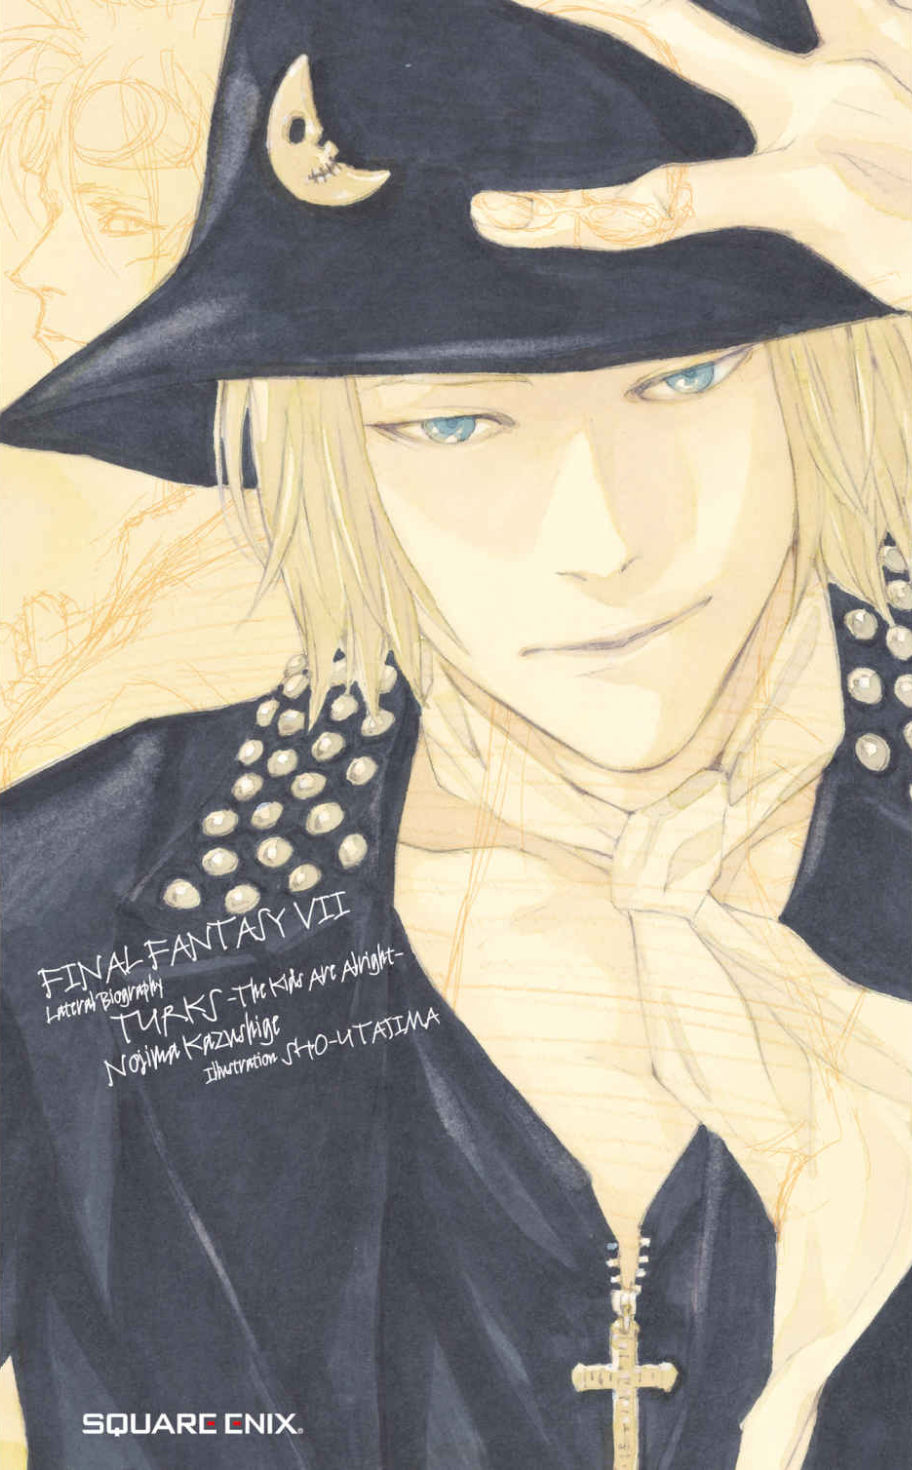
\includegraphics[width=\textwidth,height=\textheight,keepaspectratio]{cover.png}
\addtocontents{toc}{\protect\hypertarget{toc}{}}
\tableofcontents

\chapter{First Off, A Little About Myself}
When I was fourteen, I took in this jet black cat. I found him on the roadside making the most pathetic meow you could imagine, and brought him home. While I was busy trying to think of a cool name to give him, my mother started calling him Blackie. That was the kind of person my mother was. It’s a black cat, let’s call him Blackie. I complained, but in the end couldn’t offer up an alternative.

Blackie completely ignored the chair and cushion we prepared for him, moving to a new spot every few hours. He would go all around our cramped house―from the kitchen, to my room, to mom’s room―pondering cat stuff and sleeping. Then half a year later he must have come to the conclusion that he didn’t belong here, because Blackie disappeared somewhere. I was fifteen. I don’t know how old he was.

“Maybe he didn’t like it here?”

“That’s what boys do, they leave home,” there was a knowing look to my mother’s face when she said this one night while we were reminiscing about Blackie. I’d never even thought of leaving home and leaving my mother behind. I wanted to start earning my way so I could help her out.

My mother worked in a cafe during the day, and in a bar from the evening until late into the night. She was constantly exhausted. Nevertheless, whenever I found a job, she would make up some excuse and stop me from taking it. I think it was down to the illness I used to have. It was my heart. But I had surgery when I was five, so it should be all clear, and since then it’s been absolutely fine. I’d been the picture of health, if I do say so myself.

“Hey, I’ve been thinking, I really do want to work. That’ll make it easier for you, won’t it?”

“Thank you. But in two years. When you’re seventeen,” Mom said as she played with the waves of her hair. She had beautiful blonde hair, but it always reeked of tobacco smoke.

“Why seventeen?”

“Because I’m sure Blackie was seventeen too.”

It didn’t make any sense at all. Why would working and leaving home mean the same thing? I thought we should have talked it out, but it was painful to talk with her when she was drunk.

Half a year later, I saw Blackie in the street. Well, a cat that looked like Blackie. He had turned into a stray, missing the tip of one of his ears and covered in scars. I called out to him and he just looked at me without a hint of enthusiasm, then looked away and started walking off. I followed him and, without even turning around, he climbed up the fence of a nearby house and made his way up to the roof. He was now completely out of reach.

“I want to work”, “Wait a bit” – the same conversation played out at regular intervals. Most of my friends were working, and even if they weren’t, they must have at least been earning their own spending money. It felt like they were all up there on that roof, laughing at me.

This was in Sector Six of Midgar. At the end of a busy street lined with shops and restaurants. Our house was just down an alley, nestled between a bookshop and a weaponsmith’s, that was damp and reeked of rust. Houses with the kind of basic shapes you’d see in a kid’s drawing, made of some material that looked like brick, were bunched together. It was apparently used as a housing area for lower-level Shin-Ra Company employees for a while after Midgar was completed. Later on, company housing was moved to Sectors Seven and Five. The area was supposed to be demolished, until some rich guy who ran a couple of bars leased them from Shin-Ra for his workers to live in. The rent was dirt cheap. A lot of the people who had come to Midgar from the world below – rural areas or the slums – with dreams of making something of themselves lived there. Everyone was poor. This was the sort of place for people who didn’t make it among the relatively wealthy populace of Midgar, but everyone agreed that it beat living in the slums.

It was about one week before my seventeenth birthday. The sound of the phone woke me up. I could hear Mom talking to someone in a quiet voice. When I got up, she was cleaning the kitchen/dining room. Cleaning and tidying – in other words, maintaining order in the home – was my job. Studying at my teacher’s home, talking with my friends, wandering around town. Staring at a TV with bad reception. For someone all but devoid of actual responsibilities, cleaning and tidying was my sole contribution to our life. I’d never cut corners there. When I argued that I had done it yesterday, she told me that we had a guest coming over.

“I’d like you to meet him, so can you go get changed?” she said, without looking at me. Something felt wrong about it, and that hunch proved true.

Nick Foley was in his mid-thirties, like Mom. His tall frame was covered by a well-tailored grey suit. Above a light-pink necktie with white dots sat his little, clean-cut face. He stood in the doorway, a pleasant smile across his face as he looked down at me.

“Call me Nick. I work in the Shin-Ra Company’s business department.”

With the way he was smiling and introducing himself, it was like he was saying ‘Hey, we’re friends now, right?’. If I’d let my guard down, I might have actually ended up calling him Nick.

“You take after your dad, don’t you?” judging from the look on his face, Nick Foley wished he hadn’t said that.

“You knew my dad?”

My dad died in Wutai right before I was born. There wasn’t even a single picture of him, so I didn’t know what he looked like.

“What, no, I just meant that you don’t look much like your mom. I’ve heard what happened... sorry. But you’re a good-looking boy, aren’t you? I bet you do well for yourself with the girls.”

I must have been making quite a face, because Nick Foley started looking at my mother for assistance.

“Do you want some of this cake Nick brought? It’s from Mrs. Tosca’s!” she made too much of a noise as she set the plates on the table and placed a slice of that overly decorated cake on them.

Eating one of Mrs. Tosca’s insanely expensive mounds of sugar and cream was a treat my mother reserved for when she got paid. She liked to take her time to enjoy it, this little reward to herself.

“Come on you two, sit down.”

“So here it is. Been wanting to try one of these cakes ever since I heard about them. Normally I don’t care for sweet stuff at all,” Nick sat down in my seat as he rambled on about some pointless crap.

Please just die.

The smile vanished from my mother’s face.

There were three chairs around the table. Out of the remaining two, I took the seat opposite the enemy. My mother’s seat. She sat in on the chair saved for the rare visitor we had.

Nick Foley must have noticed the chill in the air too. He let out a heavy sigh and looked right at me. He put his elbows on the table and folded his hands in front of his face. “I had wanted to meet you a lot sooner, but I could just never find the time. It’s really cutting it close now. You’ve heard about me, right?” Nick Foley looked at my mother.

In a barely audible voice she said she was sorry, she couldn’t bring it up.

“—Great. But the arrangements are all set now, so we can’t move the date. We’re leaving Midgar in two days. Get your things ready.”

“What are you talking about?”

“I’ve talked it over with your mother several times. You’re just going to have to come along. You are family, after all. I’ll be heading off now, but if there’s anything you want to know more about, your mother will—“

I swept the cake off the table along with the plate and slammed my foot down on the floor as I got up, then went straight out the front door.

The sound of the plate shattering rung in my ears. I felt bad about doing something so unlike me.

When I’ve calmed down, I’ll go home and talk to Mom. There seems to be a lot of stuff I don’t know. But still, leaving in two days? Leaving to where? No. It doesn’t matter where, I don’t want to go. I’m not going anywhere with him.

I decided to kill time for two days, then go home. If I did that, Nick Foley and my mother’s plans would be shot.

It’s probably going to be a little awkward for a while, but what can you do? Things will get back to normal soon enough, I kept thinking to myself as I walked through Sector Seven to the warehouse block in Sector Eight – the usual destination for teenage runaways.

And then I got caught in the infamous Sector Seven plate incident. There were a number of support struts that held the massive weight of Midgar’s giant, circular base from the ground below – one for each of the eight Sectors. This was the incident where the seventh of those struts was blown up by terrorists. Having lost that support strut, the Sector Seven plate, in its entirety, became severed from the flanking Sectors Six and Eight and fell. It flattened the slum below, obliterating it. A lot of lives were lost.

At the moment of the explosion, I was at the border between Sectors Seven and Eight. When the city shook from the blast, I instantly ran away in the direction of Sector Eight. At first I had no idea what was going on. I ran without thinking, following the droves of people. Eventually I learnt that Sector Seven had collapsed. There was news that Sector Six was safe, but nothing was certain. I was worried about my mother. I tried to go back home via Sector Zero in the center of the city, but that route was sealed off by the Shinra Army, on the lookout for the terrorists. Having no other choice, I decided to work my way backwards, going through Eight, One, Two, and so on. The people were afraid of where the next explosion would be. These deranged terrorists had only just recently blown up the Sector One Mako Reactor.

It took me three days to reach home, after having gone nearly full circle around Midgar. What would have taken one day of walking without resting, had I been able to go the shortest distance, took three days. I got lost in the unfamiliar streets of Sector Eight and got into a panic. Before long it was night. The cold breeze that came from the gaps between the warehouses mercilessly sapped the warmth from my body. First, I was hit with stomach pains. Then, it was fever and chills. Cursing my body for its weakness, I looked for a place to lie down. Finally I stumbled across an empty warehouse, and collapsed onto an abandoned mattress. Then, out of nowhere, a couple of guys appeared, looking at me with nasty glints in their eyes. They were the same age as me, but if I were a house cat, these were strays. They insisted I pay them to use this spot, claiming those were the rules around these parts. But I had no money or valuables on me. In the end, giving them someone to vent their dissatisfaction on was how I paid up. The pain where they had kicked my back and stomach was killing me.

One night’s rest didn’t do much in the way of making me feel any better, but I didn’t want to pay the charges again to stay here another night. More than worrying about my mother, I just wanted to go home. I mustered up the energy and left the strays’ den.

I staggered along, taking frequent breaks on the way, and managed to arrive home past noon on the third day. The house was okay. Mom was out, but this was usually when she would have been at work. I took some cold medicine and crawled into bed. I fell asleep, having decided to go see my mother when I got up. It was night-time when I woke. I still wasn’t feeling great, but probably good enough to make it to the pub and back. First I took a shower. I dried myself off with a towel and went back to my room, put some underwear on and some black pants. I picked an oversized sweater that hid my body to wear on top, a navy blue one. This was the most grown-up combination of clothes in my wardrobe. My tall-but-lanky build was the target of ridicule at the pub. I was certain to end up barraged with the same old remarks, telling the kid to have a glass of milk and run along to bed.

Just as I was about to head out of the door, the messy state of my bed started bothering me. When I straightened out the thin blanket and fluffed up my pillow, I noticed an envelope that had been placed under it. Inside was a large sum of money and a letter from Mom. I read the letter.

“I’m going with Nick as we planned. We will contact you to tell you where we are as soon as we have settled down. Use the money in the envelope to live on and wait for me to call. Leave half of it to pay for the trip to our new home” – the whole thing was utterly impersonal and businesslike. The Sector Seven incident had happened on the same day I ran out of the house. She must have known about it and the extent of the damages. But she left with a man without even making sure her own son was safe. And she seemed to think that I would just come running when she tells me where she is. I didn’t get it.

I went to my mother’s room and opened the closet door. On the hangers were a few outfits for her daytime job that looked a bit too youthful for her age, and several horrible ones for her night job. It looked like she’d left her work behind too. The clothes she wore off-work, which were usually strewn in a mess beneath them, were gone. I sat on my mother’s bed for a while, absent-minded. Then I suddenly remembered our family’s little secret, hidden in the ceiling.

I brought a chair in from the dining room and placed it in the middle of the room. I got up on it and stretched out my hands, removing one of the ceiling tiles. I gently threw the tile onto the bed and looked up at the square hole that had opened up in the ceiling. Mom had hidden a chest there. Inside there was money and treasures. The money was her weekly wages, and the treasures were my “first somethings” – my umbilical cord, hair from my first haircut, the first baby tooth I lost – each one creepy any way you looked at it, but to my mother I guess they were all irreplaceable treasures.

As I stuck my hand into the ceiling my fingertips hit the chest. It seemed to have been pushed back and I couldn’t reach it. I grabbed hold of the edge of the next tile with both hands and lifted my body up. I was going to stick my head in to check it out, but the tile broke. I fell downwards, losing my balance atop of the chair, and nearly tumbled over as I landed on the floor. In front of my eyes were pieces of the broken ceiling tile and the treasure chest. There were also two paper bags. When I opened the chest – an old wooden cheese box that I had drawn the purple apples I used to like on in crayon when I was little – all the treasures were still safely there. There was also what appeared to be the remainder of mom’s wages. In other words, the money under my pillow wasn’t the money that was here. Where had it come from? Nick Piece-of-Shit Foley’s wallet?

Next, I opened one of the unfamiliar paper bags. It was white and brand new. When I looked inside I couldn’t believe it. Mind-boggling would have been the perfect adjective to describe the amount of money in the bag. I could live comfortably for a whole year with it. The bound bundles of money, like the bag, were new. The wrapper on one of the stacks of bills was loose. It seemed the money under my pillow had come from here. I felt like I had gotten to the bottom of that mystery, and it started to make sense. But that was not the heart of the problem. Where did all this money come from? I could only think of one person. Nick Fucking-Loaded Foley.

The other bag was made of a thicker, pale green paper. When I took the tape off the opening, there was a dark brown coloured leather bag inside. It had a sturdy build, with a flap that had a metal fastener, and the kind of drabness you’d expect from military equipment. It had a strap you could adjust the length of. It was the kind of shoulder bag you’d think would belong to a grown man, and a hardened adventurer at that. When I opened the flap there was a small card inside the bag.

“Happy Seventeenth Birthday. I hope you become the kind of strong man worthy of this bag. From Mom.”

My mother had prepared a birthday present for me, hidden it and left. A mother who disappeared with some good-looking man. And a son left behind with a pile of money.

How did all of this fit together?

I sat on my mother’s bed and thought about it. But it didn’t seem like I was going to find the answer. My mother would contact me eventually. I guessed I would just have to wait until then. For the time being, I decided to fix the ceiling.

I picked up the broken ceiling tile and got up on the chair, and returned it to its original location. Next, I moved on to the first tile I removed. This one didn’t want to fit in place properly. My arms started getting tired while I was working on it. I started getting irritable, and had no choice but to face up to the unpleasant reality I just couldn’t shake from my mind. My mother was short, and even if she stood on a chair she couldn’t have reached the ceiling. When I had grown taller than Mom, it was my idea to use the space behind the ceiling as storage. Since then it had been my duty to put things in and out of the chest. That’s how I knew how much my mother made, how much she had left, and how poor we were.

And therein lay the question. Who put the money and the gift I just found up in the ceiling?

The tall man who looked down at me in the doorway. Nick Son-of-a-Bitch Foley. That man had been in my mother’s room while I was gone.

I abandoned what I was doing, went to front door, and yanked out the cable from the phone hanging on the wall.

They’re going to see how angry I am.

I tried to get my life back to normal. I was going to my teacher’s, talking with my friends, and even watching TV. I thought about splurging with the money, but when I thought that it might be Nick Foley’s money I decided against it. No. The truth was that I just couldn’t think of anything to do with it. In the end I put the money in the shoulder bag that I had been gifted for my birthday and decided to forget all about it.

My sleepless nights continued. One evening I struck on the idea of reading a book. Reading was my mother’s sole hobby. In her room were several books she had finished. I picked out Escape From Wutai – Part 1. Because it was the last one on the end. That’s all. It was an old novel written during the war. The beginning was filled with scenes of the Wutaians using some weird martial arts to kill the prisoners in the camps. Eventually, five of the prisoners slip past a stupid Wutaian and escape the camp. Three men, and two women. There was one man too many. I figured that someone was probably going to die. Probably this Shinra military officer jerk-off. However, the officer defied my expectations and lived, and even started pushing the other four around like he was the leader. I wished he would die soon. My wish would come true near the last page. The officer was blown to bits by one of the landmines the Wutaians had planted. The way he died shocked me.

“He was blown to bits by a Wutai landmine,” that was the only story my mother had told me about my father. Maybe she had gotten it from this novel. Did she project my father onto this man who rightfully should have died? That was probably the case. She must have really hated him. I admired how she could have raised the son of a man like that. No. Maybe it was exactly because I was the child that man had left behind that, if ever there was the need to do so, she would be able to abandon me like she had done so now. I thought I was loved, but could that have just been a mask for her hatred? I threw Escape From Wutai – Part 1 against the wall. Like I gave a damn what happened to the other four in Part 2.

I went back into my mother’s room and looked at her book collection. I could tell from the titles that they were all adventure novels. On the covers were illustrations of what looked like the main characters. They were all different sorts of characters, but all women. My mother loved those kinds of novels. She lived a real life that lacked these sorts of sights and adventures. So, though I dreaded the thought, maybe she was captivated by romance. Was life with me that boring? Was it painful?

That’s enough. My mother left, and I’m left behind. I’m just going to stop thinking about her. I need to think about living on my own.

The next day I visited the café she used to work at. The manager, a man with a square forehead and the broad shoulders of a retro robot, ranted at lengths about my mother suddenly quitting. I had kind of prepared for this, but it got to me more than I’d expected. After a stream of complaints he seemed to remember to ask what I was here for. I told him I wanted a job. From the flow of the conversation I figured I was in for rejection, but the manager called up the owner right then and there. I couldn’t understand what was going on in his mind, but then again I didn’t know how my own mother felt either – it’s no wonder I wouldn’t understand a stranger.

Surprisingly, I was able to start work immediately. There was a delivery truck that resupplied the necessary food and drinks to all of the owner’s businesses. I was given the job of being the driver’s assistant. Apparently, my predecessor had gotten a job with the Shinra Company and had just gleefully quit this job.

I had the most fulfilling of days. This was “the joy of work”. I enjoyed the total change of scenery. Of course, there was never a day I didn’t think about Mom. But still, it got me away from being affected about it 24/7. I put the phone cable back about ten days after unplugging it. Maybe my mother had tried to contact me during that time. It was also possible that the phone had rang while I was out of the house. However, the phone wasn’t the only way to get in touch. The fact there was nothing was a sign that she did abandon me after all. But, whatever. Enjoy your life, Mom. I’m enjoying mine just the way I want to.

The truck driver was a hard boss to work for, but I knew he needed me more than anyone else. I’d never had that experience before in my life. Regardless of the heavy labour, I wasn’t worried about my heart at all. I’d gotten confident about that too.

What do you think about that, Mom?

I started to think those days would last forever, but the situation quickly changed. It was as if a TV flipped itself to another channel in the middle of a show. Meteor had appeared in the sky above Midgar. This comet or falling star or whatever, which had just suddenly appeared in defiance of all astronomical knowledge, looked like a massive black void in the sky. The world was ending in seven days. That was the rumor that got spread around. Giant monsters had appeared in the north and around Junon, and even the Shinra company, with all its prized weaponry, couldn’t defeat them. The city was in chaos with dodgy rumours, like you’d be safe if you hid in the mako reactors, or there was an underground shelter Shinra had built in Kalm. The only thing anyone knew for certain was that Meteor was getting closer, day by day. The initially heated debates over the truth of the Meteor and how to avoid it soon subsided too.

The owner closed his shops and left Midgar, and the neighbourhood was filled by the din of people getting ready to evacuate. My friends, the truck driver and my other workmates asked me to flee with them somewhere far away and though I was thankful for them, I declined their offers.

Seeing Meteor caused me to consider death for the first time in my life. Then, all I could think about was my mother, and the awkward circumstances we had parted on. I felt that if I left the house, I would lost all connection to her. I passed time looking at the few pictures of me and her. They were all taken at the photographer’s on my birthdays. I was standing next to my mother, gradually growing up. After I had gotten taller than her, I started pulling a sulky face in the pictures. My mother was always smiling. I looked at that smiling face and realised how stupid I had been. Mom would never abandon me. All the things I should have done ran through my mind. If I had gone to the Shinra Company, I might have found out where Nick Foley was. I probably should have put the phone cable back right away and installed an answering machine. And then the answers to the questions I didn’t even try to think about came to me – the purpose of all the money left up in the ceiling. Wherever it had come from, the reason she’d left the money was that she’d planned on coming straight back. Or perhaps she meant for me to bring it to her. That seemed likely. Mom never even considered living away from me for a long time. And then there was my birthday present. My mom took birthdays very seriously. She would’ve made some arrangement so I’d get that shoulder bag on the right day – wrote about it in the letter, or put it somewhere easier to find. But she didn’t, because she planned on contacting me soon. I should have just shut up and waited by the phone.

The joy of work? I’m such an idiot.

And then That Day came. I survived the day the mako energy, or rather the Lifestream, burst to the surface and wiped out Meteor. For seven days after that, I waited at home for my mother. On the night of the seventh day, I stepped outside and ended up going down from Midgar to the slums.

Now I’ll tell you about something that began two years after all this. I’ll probably talk a bit about some of the stuff that I experienced over the two years in between as well. I intend to follow the correct route as best as possible so as to prevent our story from getting off topic. But as I already said, I’m not great with making choices. Hopefully you’ll bear with me.

I’ll also sometimes bring up things I shouldn’t really know about. At times likes those I’ll use the facts as the basis, and use a bit of imagination to fill in the rest. For example, something like this...

\chapter{How The Trouble Began}
When Elena joined Shinra, Cliff Resort was already a long-forgotten retreat. The rugged landscape, which looked as though giants had haphazardly piled up boulders, was definitely unusual. The numerous lodges built along the naturally varied elevations in the terrain might have added some flavor to the scenery, but once you got used to it, there was nothing else there. You would visit once and take a couple of souvenir photos, and that would be enough. There was little point in returning a second time. The Shinra Company had resorts all over the world, but anyone would agree this one was a non-starter.

“I mean, really...”

Just two years ago, the Shinra Company controlled most of the world. It didn’t sit well with Elena that the President, who had been at the top of that empire, should now have to spend his days in such a desolate place as this. He was undergoing medical treatment. For security reasons, it was safer to be away from the cities, however, as it was only about a two hour drive to and from the cities it made it easy for the staff to commute. There were several reasons for them to remain there, but it didn’t change the fact it was a dull place. The name had been changed from Cliff Resort to Healen at the President’s suggestion, but that didn’t mean anything had actually changed there.

“Aaarrhh.”

Nothing ever happened here. In the square there were several benches, where the people suffering from Geostigma were sitting around, talking and laughing, some of them focusing on getting better while putting up with the pain. Things were the same as they were yesterday and would likely be the same tomorrow. Even the weather mostly stayed the same.

**

“Elena’s looking bored,” said Rufus Shinra to his subordinate, Tseng, as he walked away from the window of the lodge. “I’d like get moving on the next project,” Rufus paused as he struggled to return to his wheelchair.

“Yes, Sir. I will tell Elena shortly. However, I intend to keep this from Reno and Rude for now. This new project is more exciting – I fear if they knew the details their work in the city would end up getting cast aside.”

“Very well. Have you gathered any intel on Jenova?”

“Not yet, Sir.”

Jenova – a monstrous being that arrived from outer space. Nobody knew what form it was in now – whether it be a withered remnant of flesh, or in the form of some bizarre creature. But Tseng believed that if it were somewhere nearby – dead or alive – then surely they would know about it.

“By the way, Sir, what are your plans once we locate it?”

“My father...” Rufus Shinra answered, with his eyes seemingly gazing off into the distance. “He set his sights on the Lifestream flowing within the planet, called it Mako Energy and packaged it for the masses. Mako revolutionized the industrial structure of the day from the ground up, and mankind obtained prosperity the likes of which it had never known.”

“Yes.”

“With the immense fortune and power he gained, and even if he was lining his own pockets to some degree, my father invested most of it into new fields – on a massive scale, and without ethics. And one of those was the research of, and experimentation on, Jenova. Eventually this gave birth to a monster named Sephiroth...”

Sephiroth. That monster – a hybrid of human and Jenova – possessed unfathomable prowess in battle. His show of power on the battlefield led to him becoming lauded as a hero. However, his mind was not as strong as his body. When the hero learnt of the circumstances surrounding his birth, he avowed his heritage as the son of Jenova, and as a result went mad. He revolted against the company and, what’s more, sought the extermination of humanity. During the battle against Sephiroth the Shinra Company was destroyed, and the planet was brought to the brink of returning to stardust.

“My father took his leave from this stage early on, abandoning those of us left behind to suffer the nightmares in his wake. Far from reasonable, wouldn’t you say?”

Tseng looked at Rufus, neither denying nor confirming what he had said.

“I am not my father,” Rufus said with a forcefulness in his voice, moving his wheelchair to the window. He could see the people suffering from Geostigma in the square. “I will bring it to an end, once and for all.”

**

Elena was standing at the entrance of the woods, which stretched out behind the lodge area. The wind, carrying the scent of moss as it breezed through the trees, swayed her short blonde hair.

“Will something please just happen!”

Not the most professional of thoughts, but those were her thoughts nonetheless. After checking to make sure no one had heard her, she ducked her head slightly and started walking. As she made her way along the wide, meandering path, the largest building in the retreat came into view. Although this ‘largest’ building was still only a one-storey log cabin that could fit thirty people at the most. It had apparently been used as a recreation hall originally. She skipped for the final few steps, and stood before the door, which was securely locked from the inside. She pressed a button to the right of the door to ring the buzzer. After a full ten seconds she got an idle response from Throp,

“Miss Elena?”

He was a young man Elena’s more experienced colleague, Reno had picked up in the city.

“Making my rounds! Come on, open up!” Elena ordered, making no effort to hide her frustration.

After a brief pause, the door opened.

“All clear here, Ma’am,” Throp spoke in an unenthusiastic voice, while fussing with his shaggy, uncut hair, which didn’t seem to have seen water in a while. His massive body, towering over Elena, was as doughy as can be – his stomach made a noticeable mound under his shirt – not in the least bit cut out for guard detail, but they were short on manpower. This man symbolised the current state of the Shinra Company.

Elena weaved her way past the behemoth, stepping inside the cabin and, moving her gaze along a now-routine course, she inspected the room. From the left to the right. From the right to the left.

Yup, all clear.

Until the previous week this building had been used as a lab for developing medicines. They were developing a medication to suppress one of the symptoms of Geostigma – generalised pain. It was already known that the stimulant that the company used to issue to the members of Soldier offered some pain relief. The research team analysed that stimulant and successfully synthesised a similar ingredient. With the assistance of the patients in the retreat, they were able to perform clinical trials, and at last came up with a medicine that could be mass-produced. The manufacturing method was to be provided free of charge to small and large organizations capable of producing it, such as the World Regenesis Organization. It was Elena who proposed this project, and had travelled around to make it a reality. The staff she had cobbled together were all that was left of Shinra’s science and chemistry divisions. More than a few of the members of these two departments had traded their consciences for brilliant minds. Elena was wary of leaving them to their own devices. There was no telling what dangerous concoctions they might have turned out if left alone, so she kept a constant eye on them. But her fears turned out to be unfounded. The researchers who gathered at Healen were devoted and good-hearted. They worked practically night and day without rest, and completed the medicine in an extremely short time. Elena regretted not having trusted them, and on the day they left she expressed her respect and gratitude to each and every one of them.

The majority of the equipment, fixtures and medical apparatuses set up in the hall had been packed up, and were piled up against a wall near the entrance. They were going to be donated to those planning to continue their research on Geostigma, and to doctors in Edge and other cities who were treating patients.

On a shelf at the back of the room were airtight metal cases containing the samples of the medicine. There were two cases, one of which was for the retreat’s patients. There was a limited number of doses, so it was strictly controlled, with records kept when it was given out. The other was to be handed over, along with the research reports and manufacturing guides, as soon as the WRO was ready.

“Oh, I’ve already checked all that. It’s all fine,” Throp said to Elena as she neared the medicine shelf.

“I’ve still got to follow procedure.”

“Right, yeah...”

She picked up the distribution record without turning around for Throp’s grumbling, and opened the lid of the metal case. Handing out the medicine and recording it was Tseng, her boss’s duty. The page was lined with Tseng’s meticulous handwriting. After checking the column showing the remaining number of doses she compared it against what was in the case. All fine. Next, she checked the small thermometer inside the case. The medicine was sensitive to changes in temperature, which could alter the effects – nothing as extreme as rendering it useless or poisonous or anything, but it had been confirmed that it dulled the effectiveness. This would likely be remedied sooner or later, but for now it needed careful handling.

“You’ve been good again today. All fine,” said Elena, making sure Throp could hear her. While she spoke she looked at the other case. On the outside it looked the same, but this one was sealed up with a sticker so the two wouldn’t be mixed up.

“This one’s also fi—” there were signs that the sticker had been removed at some point. “Throp, did you touch this case?”

“Course not!” Throp denied it instantly.

Elena took the mobile phone from the holster around her waist, and called her boss, “Excuse me, Tseng, Sir? Did you take the sticker off the medicine? The batch that’s getting shipped out.” As she listened to his reply she glanced out of the corner of her eye at Throp, who was looking out of the window with a reproachful look on his face.

Why’s he looking out the window?

With an exaggerated motion, Elena turned her back to him, “Thought so. Understood, Sir!” She sensed that Throp was inching his way towards the exit.

He’s underestimated me – no, the Shinra Company as well.

“I’ll shoot,” she warned in a low voice. Throp stopped, and ducked his head down.

“Sit down there,” she motioned with her chin towards a folding chair used for breaks, and Throp sluggishly complied. Using packing rope left on the shelves, she fastened the giant’s hands and feet to the chair. “You just wait here.”

When she got outside, she started running in a different direction from the small path leading to the lodge area, heading to the boundary of the wastelands and the forest – the direction Throp had been looking at through the window. The roots of the trees were jutting out from the ground like tripwires. Dodging the roots, Elena ran through the forest like a hunting hound. When she thought about how Throp’s accomplice, or maybe even the ringleader, might be up ahead, it excited her. This was how the Turks were meant to be. The medicine development project was one dear to her heart, but it was a special assignment. It was fair enough to work for the sake of the world or for your fellow man, but first and foremost the Turks’ duty was to the Shinra Company. They did whatever it took to protect the company.

As she neared the edge of the forest, she found her prey. A chubby man who was unsteady on his feet was trying to leave the forest.

“Freeze!”

The fugitive surprisingly stopped as ordered, and turned around. It was a young man dripping with sweat. His seemingly natural curly black hair stuck to his forehead, and drops of sweat were falling from the tips of his hair. His square, black-rimmed glasses looked like they were about to slide off his round face. He was wearing a green sweatshirt and dark-green trousers, which he must have thought would work well against the woodland backdrop, however, amongst the rows of pale-brown tree trunks, he couldn’t stand out more. Seeing that pathetic sight took the wind out of Elena’s sails.

“Please, just let me go!” shouted the man, bright red in the face. Then he started running again.

“You’ve gotta be kidding me,” Elena regained her composure and gave chase. I can’t let him leave the forest. He must have a vehicle waiting. Wherever he came from, there’s no way a guy like that walked it through the wastelands.

Just as she was about to catch up to him, her phone rang. When she answered it, Tseng’s voice was on the other end. She stopped running, and looked at the back of the man in green as he ran away. He ran frantically, all the while looking as if he was about to fall over.

“...Yes, Sir. I’ll return right away.” Elena sighed as she hung up the phone.

**

“Now then,” Tseng crouched down on the spot, speaking toward his feet.

Throp was lying on the floor along with the chair, his eyes darting around the room. Blood from his nose stained the floor.

“Where does this Fabio Brown live?”

\chapter{Trouble Comes Knocking}
I looked at my reflection in the mirror and gave my nose a pinch. If my broadly spread nose had been a little bit more pointed, maybe it would have altered my past. Actually, I wonder about that. I don’t think there has been one single time when the shape of my nose was the problem. The problem was the colour of my hair. At one point I dyed it black, but I stopped doing it when a rash broke out on my head because of the cheap dye. For now, I’m putting up with the colour I was born with, a brownish blond. It’s not a colour I’m very fond of. It just makes me think of a spoilt brat who’s had an easy ride in life. That’s how it feels to me. It’s a pain to have to explain all the time that I wasn’t brought up like that. So I think I should have had it dyed it a tough guy colour to begin with. Black was the colour I envisioned on that type of a guy. Black as the night. I think I will dye it again after all. Better remember to get a quality dye this time, though.

I was now 19. It had been two years since I left Midgar. I felt I had a meaner look in my eyes compared to when I lived there. Good, that’s perfect. Get rid of anything that makes me seem like a kid. I psyched myself up and washed my face in the water I had drawn. Then, as I dried my face with the towel draped over my shoulders, I looked around the bleak, tiny room. The bare steel plates on the walls were a stark sight. More than a year after this house was built and the interior decorating had still been neglected. There weren’t any practical issues with it, but no matter how much time passed, it still seemed like temporary accommodation. If I was planning to stay here permanently, then today was the day I ought to get started. If I let a milestone such as a birthday pass me by, I could very well end up putting it off for at least another year. I had the wallpaper and paint I needed prepared by yesterday.

Well, let’s get to it.

Firm as my resolve was, once the steel plates and plywood were hidden by the wallpaper, I didn’t care any more about what happened with the rest of it. But I couldn’t call it quits there. The can for the paint I got for the ceiling was warped and wasn’t properly sealed. I had to use it quick or it wouldn’t be any good. If I wasted this, getting another would be tricky. The paint was this phosphorescent type that had started showing up on the market lately, which I’d gotten from a tight-fisted trader. At first he was asking for 1500 gil, but after I haggled with him, given the poor state the can was in, the seedy bastard sold it to me for 100 gil in the end. It was probably stolen. But, I didn’t care so long as the paint itself was the real deal.

These days, that’s how it is when you’re doing business with others – don’t think about where the merchandise might have come from. At night, phosphorescent paint emits the light it absorbed during the daytime. Considering the energy situation nowadays – there might as well not be any – you’d be a fool to get lazy and waste the paint now. I might be lazy, but I ain’t no fool.

I took my shirt off, and just as I was about to start, there was a thud at the door. I froze and looked at the door. There was another thud from the bottom of the door. The whole of this flimsy house shook.

“Fabio Brown. We know you’re in.”

My body shrunk at the sound of that low voice, calm but with a menacing ring to it. I stuffed the rag I was using as a paint brush into the paint can, held my breath, and put on the shirt I had just taken off. My hands were trembling. I let out a burp.

“We’re gonna bust down the door, yo!” It was a different guy than before. He sounded like he was laughing.

I stayed silent and looked at my boots. I had them specially made last year, using a monster hide I found in the market. Maybe the day’s finally come when I will put these pointed, steel-toed boots to use. However, I had treated them with care, so there was barely a mark on them. I’d rather avoid getting them any more scuffed if I could help it. So that leaves me with fleeing. But through where? I didn’t even need to think about it. If I couldn’t use the door, the window was the only option. The window was next to the sink. It was made to fit the size of the glass pane, so it was pretty small, but not so small that I couldn’t get through it. I quietly moved to the window. Then, I thought to take a dinner knife out of the drawer by the kitchen sink. It had a sharpened blade, about 5 centimetres long, that could also be used for preparing food. If it came down to it, I’d stab them.

“We’ll give ya 30 seconds.”

It seemed they were going to start counting down. The window was fixed in place, so I would have to break it to get outside.

You realise how valuable glass is? No, there’s no other way. But what can I use?

As I wondered if I had something hard to break the glass with, the door came crashing down with a creaking sound.

That’s not what they said. It hasn’t even been 10 seconds yet.

Stepping on the door, which had fallen inwards, a man with a lean figure and blazing red hair entered the room and grinned. He was wearing a suit with a distinctive design. He was one half of a pair of men I’d seen around a lot in the central square. Which meant the low voice I heard first was probably the big guy with the sunglasses and bald head. They were always together. Like a knife and fork.

“Drop the fork, kid. You’re gonna hurt yourself.”

The redhead came closer without showing any sign of caution. Don’t mess with me. I stuck the fork – fork? – out and thrust it at the redhead.

“Oww.” I let out a pathetic whine. My wrist had been hit by the edge of the redhead’s hand, and I had dropped the fork on the floor. While I was thinking of how things might have turned out if I had calmly picked up a knife, the redhead’s knee sunk into my stomach. Out of reflex I slumped forward, holding my stomach.

I was grabbed by the collar of my shirt from behind and pulled back into place. Then he got me in a nelson hold. With my arms raised up, I was forcibly turned to face towards the door. My feet were nearly off the ground. I was just barely standing on the tips of my toes. The redhead was picking up the door off the floor and resting it in the doorway. Which meant that the brute behind me must have been the skinhead.

“Come on now, Fabio,” The redhead moved his face closer as he prodded my chest with his finger. “Whoaa!?”

With that he went quiet, and looked at me with his mouth still agape. Before I even had a chance to wonder what the hell was up with him, the brute behind me started pushing on my neck. I couldn’t breathe. I can’t take it. It hurts.

“Give back what you stole.”

What’s he talking about? Why would I know?

But it was hard to prove that you didn’t know something.

Find the best solution. Make your choice. What’s the answer that’ll get you out of this mess?

“Come on, say something.”

The skinhead eased his grip for a second, before moving the hands he had locked behind my neck up to the back of my head and pushed harder.

“It hurts—“

“Give it back and it’ll stop.”

Muscles moved behind me, and my feet left the ground. I could feel blood gathering at my eyes. Then finally it started flowing out.

“Don’t cry now, man. That’s lame.”

Crying? I was crying?

“Hmph, stupid kid.”

All of a sudden the grip behind me loosened. I collapsed to the ground and, without meaning to, found myself looking like I was begging for the redhead to spare my life. It was humiliating but there wasn’t much else I could do. I was going to have to ride this storm out by grovelling on the floor. Just like two years ago, when the mako swept over the planet.

“Well, they are just things. I can guess why you’d do it. If you promise not to do it ever again, we’ll let you off with a little punishment.”

My body reacted of its own accord to the word “punishment”. With a burp and trembling. I’ll admit it. I might idolise tough guys more than most would, but the reality for me is quite the opposite.

“Sorry ’bout scaring you.” The way the redhead said it sounded like he was taking pity on me.

“That’s exactly what we came here to do,” the skinhead retorted.

C’mon, have a falling out and kill each other. Or if that’s asking too much, then just keep on talking. Give me time. Time to figure something out.

“Hey, Fabio. Eyes up here.”

I had to do what they said. I looked at their faces. These two men I normally saw from a distance were right in front of me. The redhead looked like a delinquent kid who’d grown up without actually growing up. The kind of guys I felt both admiration and hatred for, like the ones who had been in that warehouse in Sector 8. The perfect example of one of them was looking down at me as he smiled at the corners of his mouth. The skinhead was even larger than the redhead. Not just in height, but the sheer mass of him was something else. Even in this dim room he didn’t take off his dark sunglasses. I was sure they lived in a completely different world to me.

“We were throwing around some pretty stern looks before we got here, can’t exactly leave now without doing anything. Gotta do the job properly and show people what’ll happen if you mess with us.”

“Ar-are you going to kill me?” Those were the words my continued search for an answer dug up. And with my voice cracking at that.

“That would be the easiest thing to do. But see, what we’re after is a Shinra that’s beloved, and a little feared at the same time. We don’t want to be hated. Killing you, that’s gonna get some hate coming our way.”

“Do you know who we are?” the skinhead asked.

I gave three quick nods. The Shinra Company’s Turks. The “if you don’t behave, the Turks are going to come for you” Turks. The next generation and heir to the reins of Shinra, commonly known as the Idiot President. This was a moniker resulting from the same kind of lazy naming that lead to calling a black cat Blackie, but that was the name everyone used. The world went to hell not long after he took the position of president. Considering all that, I guess that was only appropriate. Anyway, he had been blown away along with the building, and I didn’t know what happened to the Shinra Company after that. But these two men were still calling themselves the Turks from the Shinra Company. They were using the effect that name had on regular people. The Turks were Shinra’s dark side. Whenever there was a problem that required violence to solve, they’d be there.

“Now, whooo are we?”

“The Turks... sir.”

“Cut the ‘sir’ bit, kid.”

“...Sorry.”

“Get up.”

I staggered to my feet, as ordered. My legs were still shaking. Just as I thought the redhead had moved suddenly, and I felt an impact on my face and flew into the corner of the room. My back hit the three-legged stool, one of the few pieces of furniture I had, and I fell on the floor along with it. My right eye hurt. He’d punched me in the eye. When I touched it, it was wet. Blood? I quickly looked at my hand and saw that it was the phosphorescent paint.

“Think this is enough?”

“He is getting off a bit lightly – but it’ll do.”

I rolled over on the floor and listened to their conversation with my back facing them. Soon I sensed that they were going outside. All the strength left my entire body. Strange sounds came up from the pit of my stomach, rising like bile. Was I laughing or crying? I couldn’t even tell. I pulled my knees to my chest and curled into a foetal position, and waited like that until my body and mind had settled down. Three minutes. Maybe five. And then—

“What the hell do you want!?” I shouted the words I wish I had said in the first place as I picked myself up.

“Can I ask something?”

The voice startled me. When I looked at the spot where my door had once been, I saw the redhead standing there looking at me.

“Where’s your dad, kid?”

Surprised that the redhead was still there, I couldn’t figure out why he was asking that. On top of that, I couldn’t comprehend how he was acting like nothing had happened, either.

“I’m asking you what’s going on with your dad.”

“He died. Before I was born.” I just wanted him to leave as soon as possible. Might as well just answer honestly.

“You have a photo or somethin’?”

“No.”

“What was he like? Your mom must have told you about him, right?.”

“No.”

“So you’ve obviously never met him and you don’t know what he looks like either.”

I nodded. I intended to answer honestly for as long as necessary.

“Then, what about your mom?”

“She died,” I said after a brief hesitation.

“During Meteor?”

“Yeah.”

The redhead slowly nodded at my answer. “Well, you take care of yourself. Don’t be doin’ anything stupid again, Fabio.”

With that fundamental misunderstanding left unresolved, the redhead left. I rolled onto my bed and went over what had just happened.

I should have done that. If only I had said this. All these choices I hadn’t even thought of went through my mind. It was depressing. The throbbing around my right eye was informing me of the desperate state I had been in. My stomach and my neck hurt. I got off the bed and looked in the mirror. A man who had just been punched was looking back at me.

Hey, that was a bad time for you. But it’s over now. Getting hit by the Turks, now that’s something to boast about. Well, get yourself out there.

I nodded and washed the paint off my face. Then I put the broken door back into place. It was just the nails that held the hinges in place that fell out and caused the whole door to come off. Cheaply made things have their advantages. I finished the repairs without much effort. I didn’t like leaving the paint spilled on the floor or the assorted necessities strewn around, but I was going to leave those for later. I took my jacket off the hook on the wall. A light brown leather jacket. The metal studs on the collar gave off a dull glint. What I liked best was the illustration of a monster on the back of it. A Bomb just about to detonate. It was a one-of-a-kind and cost a fair bit, but I couldn’t resist. I put it on and went to the bed, pulled out the rugged shoulder bag that was hidden under it and put it over my shoulder. Recently, the leather had softened and made it easier to use. Finally, I put on my mountaineer hat. I’d gotten it from a girl recently. Ready for battle.

My house faced out into a circular courtyard garden about 15 metres in diameter. There were six similar houses around the circumference of the courtyard. In the garden were materials someone thought might come in handy – in other words, junk was piled up. The most notable item was a car from about 10 years ago. It was a roomy, old, luxury car that seated five people. The exterior was in tatters now, and of course it didn’t run. The owner said it would run if it just had a battery, but you weren’t going to get your hands on something as valuable as that around here. The owner was a muscular man named Doyle, who was also the one who started building the houses here. We all call him the “Mayor” out of respect. He was probably in his early thirties. Normally he was a cheerful man who moved his thick eyebrows about wildly as he spoke. But behind all that, he was a really lonely guy. Just about two years ago he called some friends over to the house he’d built himself and they started living together. Well, he built the house so that he could call people over. Soon his friends called their friends, and the numbers grew, and it got suffocating in the house. They all got together and agreed to build their own houses. They shared the labour out between themselves, and built their houses next to the Mayor’s, so it enclosed the storage area for the cars and building materials. In the end, this circular courtyard was formed. When I first visited my friend who lived here, there were five houses. I was introduced to the Mayor, who then asked me if I wanted to build a house and live there, since there was some land leftover and it just didn’t look right like that, so I took him up on the offer. I became a resident of this “Doyle Village” to fill in a gap.

The red door of the Mayor’s house slowly opened, and a man cautiously poked his face out. Ratface. He had a short, shabby frame. His rigid-looking hair was grown out on all sides, and just made his head look a lot bigger than the rest of him. He was maybe the same age as me. I’d started seeing him around about a week ago. He was always wearing a dark grey work outfit.

“Hey, you’re alright! That’s a relief.” He looked like he knew what had gone down.

I put my hand on the swollen, painful right half of my face, and sent him the message that it was a bit too early to give it the all-clear just yet.

“Wow, they really did a number on you, didn’t they? The Turks turned up at the door, so I ended up giving them your address without thinking. You seem like you’re used to it, so I figured you’d be fine – sorry ’bout that.”

“Well, I’d say you were right in thinking that.”

For the most part, that was how I really felt inside. I liked the reason he gave for telling them my address. The fruits of my daily image-building.

“If you’re gonna go get them back, I can make you a bomb.”

“A bomb?”

“You know, the bombs they use for blowing up all the crumbling buildings and stuff. I make ’em.”

I told him I’d think about it, but I had no desire to involve myself with the Turks any further. The man gave me a solemn nod and closed the door. I locked my own white door, and knocked on the green door of the neighbouring house.

Then I called out to my friend, “Fabio? It’s Evan, open up.”

My name is Evan Townshend. It’s the name I’ve had since the day I was born.

After a short wait, the door opened slightly. As I lowered my gaze, I saw a face looking up at me from waist-height.

“Hi, Evan.”

“Hey.”

Vits Brown. Fabio’s little brother. He looked like a mini carbon copy of his older brother. The brothers lived here on their own, surrounded by green stuff. Their parents had passed away two years ago. Apparently they were crushed along with their house when Sector 7 fell. The brothers were saved thanks to being in the Sector 3 slums. Apparently, there was a house there that had a garden with all these flowers everywhere, and they had both been admiring them. Of course, it wasn’t the flowers they were looking at, but the green leaves.

“Where’s Fabio?”

“He’s gone out. It’s work time now, isn’t it?”

“Oh, yeah, it is.”

“What’s wrong with your eye?”

“Oh, this? I tripped. I was on a chair painting the ceiling and lost my balance.”

“Ooh, there was a real big noise. It woke me up.”

“Sorry ‘bout that.”

“That’s fine. What’s the point in sleeping when it doesn’t hurt with this medicine? I wanted to go somewhere, but Fabio told me I had to stay in while he’s gone. I fell asleep reading a book.”

“Medicine?”

Obviously it was medicine for Geostigma. Vits’ symptoms consisted a lesion called “Geostigma” that covered his skin from his hairline to above his eyebrows. One had been developing on his back too, apparently. Also, there was this black fluid that seeped from the lesions. The amount varied from day to day, but they say it’s quite painful.

“They’ve made a medicine for Geostigma? I hadn’t heard anything.”

“...” Vits averted his gaze like he’d done something wrong.

“Fabio told you not to talk about it? Even to me?”

“Well, I guess you’re okay. It’s actually this latest medicine they just made. It doesn’t cure it, but it makes it stop hurting. They call them a-nal-ge-sics, right? Fabio got it especially for me, from a doctor.”

His face was full of pride. I get it now. If there was a good reason for me to have to suffer the violence and humiliation, then I was fine with that.

Edge. That was the name people recently started using for this city. Up until two years ago this area was just a wasteland. A barren land that stretched out from the east side of Midgar, a city of steel and iron. Now, it had become a fine city. Construction on several larger buildings had started as well. I didn’t know why they needed so many tall buildings when there was all that empty land around, but that had nothing to do with me. They could do whatever they pleased. Edge was a city of freedom.

I walked down the main street to the central square. This main street, which extends out east from Midgar, was initially used for transporting building materials. Once the sides of the main street were filled with houses they built with the materials that were brought here, the city proceeded to expand outwards in a radial pattern. The landscape was changing with each passing day. If you stood in the same spot every day, you would see the flourishing growth of the city. I’m normally the type of person who is quick to criticize, but I couldn’t help but be speechless at that sight. You could feel the positive energy of the people. Whenever you’re feeling tired, just look at the city.

\chapter{At Seventh Heaven}
The quickest route from Doyle Village to Seventh Heaven, our meeting place, was to cross the central plaza. Nearly two years ago, an officer from the Shinra Army who was said to have returned from the fortified city Junon declared that this spot would be the centre of the city. Because of that work began on making it into a plaza. The officer’s men and volunteers took part. Shortly after the officer disappeared, and later on there were rumours going around that he’d been killed. Guess it was some infighting between the remnants of Shinra. The project itself was taken over by volunteers, and the plaza was basically finished. But even now you still see about fifty volunteers working there every day. Some days there’s more than a hundred. They were building a memorial in the plaza. Something in honour of the souls of the victims of the Meteor disaster, they said. You can’t say anything against the sentiment. But there was just something about those guys that didn’t sit well with me. I hated the atmosphere they created. It seemed like they were trying too hard to show everyone what positive and upstanding lives they were leading, for the world, for the people, for the future.

“Hey, matey.”

The red-haired Turk was leaning against the framework of the memorial in the centre of the plaza and looking at me. And beckoning me with his hand. Smooth move, Evan. Of course they would be here. It was the Turks who were managing the construction. What did the Shinra Company think they were doing in this day and age? All those volunteers were a pack of little animals who couldn’t live without Shinra looking over them. That was one of the reasons why I didn’t like them.

“You fancy joining in, Fabio?”

Things would probably get awkward if I refused them. But I didn’t want to be part of their little crew. When I was walking along while trying to find the best answer, someone seems to have called the redhead and he went back to his work. I kept on walking, praying that the steel bars of the frame would collapse and Redhead would die.

I circled around another third of the parameter of the plaza, and entered one of the roads that radiated out from it. This street, one of the the first built in this town’s still short history, was my favourite. It had the nicest paving job of any of the other streets, and a lot of the houses that lined each side were so fancy, so refined that you’d have no idea they were made with scrap materials. You could walk the entire street in a matter of minutes, but for those few minutes it felt like you were back in the old Midgar. It felt like Sector 7. Hatred for Shinra aside, Midgar was our home.

Seventh Heaven, a diner we often used for work meetings, was located on this pleasant little street. Its beautiful proprietress was a woman in her mid-twenties called Tifa, who had a fine ‘endowment’. Helping her out around the shop was a little girl called Marlene, who despite her moments of sass had a face that guaranteed she would grow up to be another beauty.

“Welcome!”

Tifa greeted me with a soft smile. Lots of guys would probably have their eyes drawn a little further down, but for me it was her gentle smiling face that gave me comfort. She moved her gaze, pointing me towards the table where my friends were. I gave a silent bow in return. A little ritual we had repeated many times. Neither was looking for or expecting anything more. This was part of being a regular customer.

My friends were sat around the table. The one in black-rimmed glasses with his round face pointed in my direction was Fabio Brown. Vits’ older brother. You’d usually find him wearing green clothes. Today he was in a light green shirt. It’d probably love to wear a pair of green glasses frames if he could get his hands on some. Fabio hadn’t noticed me, and was staring at the coffee cup in front of him. He must have been worrying about his brother. Or maybe he was regretting stealing the medicine from Shinra. The guy with the short grey hair sitting on Fabio’s right was Lesley Kyle. His dark, rough skin went well with his hair colour. His deep-set eyes and tightly closed mouth gave the impression of a man of few words, but the reality was a different matter. He was a font of knowledge and surprisingly outgoing, and as a result he was the guy you went to if you wanted information. He was propping up his chin with his hands and had his eyes closed. For some reason he always looked sleepy lately. And with her back turned towards me was Kyrie Canaan. The same racing jacket as always. He had cut off the sleeves and made it into a sleeveless top. The ends of her shoulder-length hair were curled inwards today. She had her elbows on the table, and her hands together in front of her face. Probably looking at her nails. Her wiggling her slender shoulders was, ten to one, evidence that she was singing something in her head. The song was no doubt the song from the Costa del Sol commercials.

“Hi.”

I approached the three of them, who would never have noticed I was there, and called out to them. Lesley looked at me and frowned. He probably noticed the change to my face. Fabio mumbled a reply with his eyes fixed on his coffee. Fabio, dude. Look at me. Pay attention to the tragedy that is my face.

“See, that hat does look good on you!”

Kyrie was in high spirits.

“Yeah, it’s not bad.”

Moving the shoulder bag I had on my back in front of me, I sat down in an empty seat.

“What happened here, Evan?” Kyrie said, bluntly point to my face. Her big eyes grew even wider.

“Well, actually...” I started to open my mouth, then noticed that Fabio still hadn’t lifted his head up. That’s not on, Fabio. “More importantly, Fabio, how about telling me when you’re going out?”

“Oh, sorry.” Fabio slowly lifted his face and finally looked at mine. “What happened to you?”

“Two Turks came by,” I said as if issuing a challenge.

“Does that mean—“ Fabio said anxiously.

“Vits is fine.”

Fabio was visibly relieved to hear that his brother was safe.

“Don’t just have your own private conversation here. You mean the Turks-Turks? What do you mean, Vits is fine?”

Here we go. There is one reality, and as many truths as there are people. I think it’s time to tell them my truth. I started from the point where the Turks showed up at my house. I took care to make sure what I said and did didn’t sound pathetic. Plus I played up the brutality of the redhead and the skinhead, and to finish off ordered a black tea from Marlene as she passed by.

“I’m sorry, Evan. It was all my fault, I’m real sorry.”

“It’s fine. At least nothing bad happened to Vits. They don’t go easy even if they are dealing with kids, you know.”

“Fabio, what did you do?” Lesley asked. I wanted to be the focus of conversation a bit longer, but what can you do?

“I heard that some of the surviving Shinra people made a painkiller for Geostigma. That they had it stored in a rest home called Healin. I took a bit of it.”

“Dumb.” Kyrie pouted her lips. “Real dumb. And I’m disappointed in you.”

“A bunch of things just seemed to fall into place. I heard that a friend of Keough, the guy who’s been freeloading off the mayor, was working security where they’re storing the medicine—“

Keough must be the the rat-faced explosives guy who told Redhead and his bald friend where I lived.

“Keough’s friend owed him a favour, and he owed me one. We promised to make everything square if he did this. So I went there when Keough’s friend—some guy named Throp—was on guard duty and got some medicine. That’s all, basically.”

That made me angry. That’s all? Tell that to my right eye.

“Did the medicine work? How’s Vits?”

“He’s doing pretty good. But I don’t know what’ll happen when it wears off. He’s fine for a short time, but that might make it more painful the next time.”

“Guess it’s only temporary in the end.”

“It’s better than having nothing at all.”

It didn’t sit well with me that the conversation was just going to end if it carried on like this. Time to drag up a few things.

“But everything isn’t square, is it. The Turks showed up. And they were looking for you specifically. How’d they find out your name and where you live? It is really all over?”

“Oh. Throp must have talked. Maybe they tortured him—“ Fabio put his head in his hands and grabbed at his hair.

“I’m sure it’ll be fine,” Kyrie said softly. “Sure, this Throp might have had to pay a price for this. But see, Evan is here, isn’t he? Punched up, but he’s still breathing. So that means they had their fill of punishment with a couple of punches, right?” Kyrie offer Fabio a lifeboat to rescue him from his guilt.

“But the Turks are a cold-hearted band of killers,” I said to sink Kyrie’s boat.

“Listen to me, Fabio,” Kyrie continued paying no attention to me. “Don’t be thinking about going to save Throp or anything. Shinra aren’t people you want to mess with, but besides that Healin is a long way away, right?”

“I managed to hire a small truck through one of Keough’s contacts. They took all my savings, though.”

“There’s monsters along the way too.”

“I didn’t see any. I guess being a nice person pays off.”

Fabio, no. Now’s not the time for your little catchphrase. Kyrie seemed to be thinking the same thing, furrowing her brow.

“I think this matter’s over and done with too,” Lesley chimed in after having listened in silence. “From what I’ve heard, they’re getting a system together to mass produce that medicine. If they’re going to be distributing it all over, there’s no point in them fixating on the amount Fabio stole. They’ve dealt out their punishment, even if it was to the wrong guy.”

“They just planning on trying to make a profit from this, right?” Fabio raised his voice. “First it was energy, now it’s medicine. They’re scum, Shinra.”

A Shinra hater through and through. There were apparently rumours that the collapse of Sector 7 was done by the Shinra Company themselves, which Fabio firmly believed.

“But Fabio, it’s kind of surprised.” Lesley stuck out his left hand in its black glove and calmed Fabio down. “The WRO are making the medicine, and to top it off they’re going to be handing it out for free.”

“No way!”

“You don’t get something for nothing.” I couldn’t keep quiet. “And the leader of the WRO used to be some Shinra big shot, you know? In the end they’re both connected. They might be camouflaging it well, but they’ve got one goal. Welcome back to the world brought to you by Shinra!”

Maybe my voice got too loud. I could feel the customers around me staring.

“I don’t think the WRO are bad? They’re goal is public security, right?” Kyrie shot me down. I couldn’t back off now.

“And soon that’s going to turn into maintaining order. Those guns they have pointed towards monsters now are going to start pointing at the cities.”

I didn’t have a shred of evidence. Even I thought I had gone too far.

“What’s with you, Evan? Giving me a hard time.”

“My eye hurts.”

“I don’t care if it’s Shinra or the WRO. It doesn’t matter what turns up is one of those groups worried about tomorrow’s world that spring up everywhere then disappear. It’s a good thing to have lots of options. We’re in a time where we can build a life with our own hands. Let anyone who wants to do it have their way. If I think it’s good then I’ll support it, and if I don’t like it I’ll turn my back on it.”

Lesley’s personal mantra on full show now.

“My eye hurts.”

I knew I was pushing the matter. I thought Lesley had a point. But I couldn’t stop myself any more. Someone please help me out.

“And speaking of Shinra,” Lesley looked at me for a second then carried on. “Kyrie said before that they’ve had their fill. That’s true, but I think they’ve got a more serious problem on their hands. The reason they didn’t kill Evan was because if they start getting a bad reputation it’s going to mess things up for them. That’s the major reason. Why? The guys using the Shinra name don’t have the power to refute and quell that bad reputation.”

“That sounds good and all if that’s the case—but that’s just you guessing, isn’t it?” Fabio said, sounding worried.

“Think about it. They’re using a guy who’d help out a thief just to repay a debt to a friend to guard their precious medicine supply. What does that they you? They’d let a chocobo watch their greens nowadays.”

“When you put it like that, that’s true.”

Fabio was satisfied with the answer, and Kyrie looked at Lesley like he was the most dependable man in the room.

“You sometimes see others using Shinra’s name besides the Turks at the plaza. But they don’t have a great influence. Have you ever thought about the reason why?”

Kyrie and Fabio shook their heads. I nodded. I’ve done it now. But Lesley began talking—

“When you say Shinra, you think of that big massive company, so you just don’t know any more. But remember, Shinra is someone’s name. The first and second generation. These two were at the heart of the world. Now they’re treated like total monsters, but that father and son essentially pulled the strings in the world. Setting aside the lower level employees, the higher up you go the more they feared and adored the president. People call Rufus the ‘stupid president’, but I think he had to have been really smart. Wish I could have met him once.”

“He was pretty handsome. Come to think of it, doesn’t Even look a bit like him?”

“What’s that supposed to mean?”

“Just joking. So, what’s the reason Shinra can’t grow any bigger?”

“Their stupid president—“ I had no option but to take what Lesley had said and take a shot in the dark. “Rufus Shinra is dead and they don’t have anyone with his charisma to take centre stage, so there’s no appeal to their organization. They can’t gather people to them.”

I was revealed when I saw Lesley nod.

“Wait up. Then who made the Geostigma medicine?” Kyrie asked Fabio.

“That was apparently some former Shinra scientists, and the Turks who had arranged a lot of it. They haven’t even seen the president.,” said Fabio. I guess he heard that from the now captive Throp.

“Hmmm. So basically, there’s nothing to fear from Shinra. That about right?”

“It wouldn’t hurt to be cautious, but it’d probably fine,” Lesley looked at me after he said that. “Even so, I’m pretty impressed, Evan. You took all that without even saying they had the wrong guy. Knew you had it in you.”

How about saying that stuff first next time.

“I’m really sorry I got you wrapped up in this. I promise I’ll pay you back somehow. I swear my life on it.”

Fabio lowered his head.

“Don’t go swearing stuff like that away.”

I pressed on the lens of Fabio’s glasses with my finger and smudged them.

“Cut it off! You know I hate that the most!” Fabio protested as he laughed. Now we’re square.

“Then I call today’s meeting to a close!” declared Kyrie. The men stopped laughing and focused on her.

“What about work? The strategy meeting?” Lesley asked the natural question. Everyone had gathered for that.”

“About that.” Kyrie dropped her gaze. “The client is coming by today, after this. I mixed the dates up, thought it was yesterday.”

“So then there’s nothing for today?”

“I suppose that’s the case.” Even though it wasn’t even cold, Kyrie rubbed her bare shoulders. “Well, let’s get off. Evan, you come with me and hear what the client has to say. It’s a man, so you know.”

“Alright, I guess.”

“If only we had a phone. Could just get in touch like that.”

Kyrie sighed. Phones were a difficult matter. Used to be that we all took them for granted and everyone had one, but with no one making them now they were in very short supply. The people who still had them from before the Meteor disaster would never get rid of theirs. When they do happen to show up on the market, it’s usually accompanied with a ridiculous price tag. But even so they soon disappeared from the shelves. Then at other times shops will be flooded with ones found in a warehouse somewhere that are practically been given away. If you’re in the right place, you’re in luck. If you can tell just how lucky or unlucky someone is by whether or not they have a phone, then we’d be a pack of unlucky ones.

“Let’s go, then.”

Kyrie got out of her seat, and headed for the counter. Lesley laughed about today being the boss’s treat, and Fabio was giving a little clap.

After parting with Fabio who was going back to Doyle Village, Kyrie, Lesley, and myself made our way towards the slums. The office we used for business was located in the slums. We could have our meetings there as well, but we all like to meet up and talk in Seventh Heaven. Of course we liked the shop itself, but there might also have been a slight sense of superiority from going out of our way and paying money to eat and drink or talk about work. I don’t know about others, but there was one for me at least. My little secret.

“You think we’ll make money on this next job?” Lesley made the effort to sound nonchalant.

“The Mrs Rich from before introduced him, so maybe we can get our hopes up.”

All female clients who look like they have money are a Mrs Rich.

“I hope so. I want to save up a bit of money. I started living with a woman.”

“Wow,” Kyrie made an exaggerated spin and showed her surprise. “Since when?”

“About two months ago. The truth is, she’s pregnant. Going to give birth in seven months.”

“No kidding—“

I lost the words to say at this unexpected confession.

“That’s great, Lesley. Really great.”

When Kyrie broke the silence after walking for a while, her voice was cracking. Lesley teased her, asking what she was crying for. There’s just been so much that’s happened, and remembering all that—

“What is she like?”

I cut in. Kyrie and Lesley had known each other for a lot longer than I had known them. I had not once enjoyed their talks about the past.

“Her name is Marle. I’ll introduce you all sometime. Ah, sorry, but I’m going to stop by somewhere then head home.”

Lesley cut off the conversation and hurried off. Kyrie and I followed the back of him with our eyes from where we’d been left. The grey haired man was heading towards an old woman selling fruit from a small wagon. Probably a rip-off merchant. Since two years ago fruit hasn’t ever been cheap. Even stuff that has almost no flavour which wouldn’t get looked at twice in the past would fetch a high price.

“If he keeps that up, no amount of money is going to be enough.”

“Yeah, maybe we ought to find more work.”

We stood side by side, watching our friend bartering with the old woman. It was a sight to see Lesley gesturing to get across the situation with his pregnant lover. They seemed to reach an agreement at last. He received two red fruits and paid his money, and started to leave. Just then the woman called him back, and handed Lesley three small yellow fruits.

“I wonder if he’ll still stick with us in the future.”

“We’ll deal with that when the time comes. I’ll work twice as hard as I do now.”

Kyrie didn’t answer me, and started walking. With a feeling of discomfort I followed her.

\chapter{Elena’s Frustration}
“Oookay, understood.”

She spoke in a bubbly voice into the phone but Elena neither understood nor was she convinced. Seems Reno had let Fabio off with a single punch. Even if they weren’t going to take his life, Elena thought it was for the good of Shinra, and of the Turks, if they at the least made it so he couldn’t get out of bed for a month.

“What’s gonna happen to me?” Throp, who had been tied to a chair since yesterday, said in a pitiful voice. The blood from his nose had dried into a dark stain on his cheek.

“I guess you’re going to die?”

“Please spare me. I was in the Shirna Army. We’re on the same side, aren’t we?”

He was one of the worst kind of men. They might be out there somewhere sullying the name of Shirna. Elena took leather gloves out of her back pockets, put them on and stood in front of Throp.

“What are you doing?”

Rushing to turn around to the voice from behind her, she found Tseng standing in the doorway.

“I was—“ I couldn’t stand it. Elena swallowed those words, slipped past the side of her boss, and stormed outside.

\chapter{Mireille Detective Agency}
Kyrie and I walked at the end of the main avenue... People from the slums call it the start of the street... In other words, we were walking at the border between Edge and the slums. The atmosphere of the town changed completely here. The slums are like a huge maze. Kyrie advanced with ease through the labyrinth. I watched her feet move as if she was walking up steps, and inched after her. I liked to walk behind Kyrie. The reason, I can’t say.

“Fabio swore he wouldn’t steal anymore.”

“But if it’s for Vits, it can’t be helped. If it were me, I’d do the same—”

I wouldn’t. No. I couldn’t. Sure, I’d plan it, but at the same time, I’d find a reason not to go ahead with it. That’s what I think, anyway.

“It’s against the rules, so what are you gonna do? In reality, he’d be fired.”

“I’ll let it slide. We wouldn’t have anyone left.”

“The lifestream says...” Kyrie said suddenly. “Evan will stay here forever, because he knows this is the best place to be.”

Wouldn’t it be great if that prophecy was true?

“The Lifestream doesn’t do prophecies. There’s no such thing.”

“It would be awesome if we could make predictions. Then we’d be filthy rich, right? Livin’ it up in Costa del Sol.”

“Nah, we’d be lynched and hung from Midgar’s pillars.”

“Scary.”

–

We— Kyrie, Lesley, Fabio and I— run a detective agency. Mireille Detective Agency. It’s got a nice ring to it. Mireille is a name we borrowed from Kyrie’s grandmother. The old lady spent her whole life as a crook. I guess it wasn’t the best name for a detective agency, but Kyrie liked it. By the way, Kyrie’s parents were skillful... not sure if that’s the right way to put it... but they were pickpockets. Before she started doing detective work, Kyrie lived a life of crime, as if it was the natural thing to do. You can imagine how we met.

Mireille Detective Agency’s main business is finding missing persons. It’s been nearly 2 years since we opened. There were many more detectives during the year after Midgar’s collapse. Seemed like half the population were our rivals. There were a lot of people with too much time on their hands, as well as a lot of people who were looking for someone or something. There aren’t many detectives these days, nor clients for that matter. It’s because the world has calmed. Most people and things are settling down in the right place. Things are falling into place. But it’s not a complete loss. Even though demand has fallen, we still get by, thanks to some creative business ideas.

‘We read the Lifestream’

That’s the slogan we use for Mireille Detective Agency. Kyrie’s use of her special ability, to access information hidden in the lifestream to find missing persons or items, is our selling point. Kyrie proposed the idea about a year ago, after 17 days without a single client. Of course, she wasn’t born with this ability. Nope, not even now. Lesley found it interesting, but Fabio and I were skeptical. Who the hell would believe that? But, surprisingly, it was right on the money. As it turns out, a lot of people believe stories that the memories and knowledge of those who leave this world merge with the lifestream. It was almost as if I was simply ignorant of the fact. In reality, there was even less than a 20% chance of us finding something we were asked to. Nevertheless, stories of our few successes spread by word of mouth, and we would have one client every 2 days. We decided to get a down-payment upfront, plus contingency fees. With the down-payments alone, we were able to make enough to support the four of us. It’s not really a scam. I mean, it is real detective work, since Kyrie gathers information for the client in good faith, and she’s pretty particular about being a good detective. Sure, the ins and outs are a bit dubious, but the results are legitimate.

Many of the requests are for people or items that went missing when the lifestream surged 2 years ago. If it were limited to Midgar and Edge, the world really isn’t that big. If a person we search for is still alive, and wants to make contact, surely they would have done so by now. In the case of an object, it has either been completely lost, or has passed through people’s hands, and will never be seen again. Two years is a long time. In other words, clients who rely on us now, are people who have half given up. Or people who intend to give up if this doesn’t work. Mireille Detective Agency is the last hope for them. That’s why we search in earnest. We sincerely weave events together into a story, based on the information we all gather, and throw in elements of the fairy-tale of the lifestream. Kyrie whole-heartedly tells that to the client. Of course, whether it’s a success or failure, the client is able to go home satisfied either way. What other job can provide comfort to people like this?

“What kinda person is today’s client?”

I called out to Kyrie ahead of me.

“Today’s client’s name is Mr. Arde. Can’t ask for too much, but I do prefer when the client is female. Men always get the wrong idea.”

It wasn’t just once or twice that male clients have made advances on Kyrie.

“Well, you are pretty attractive, Kyrie.”

As usual, I give the most neutral of favourable responses.

“Oh, thanks very much. Although, Leslie says I leave myself too open.”

One vote for Leslie.

“Well, I’m with you today. Nothin’ weird’s gonna happen.”

Here’s hoping Mr. Arde’s a wrinkly old guy.

–

The office is located in a secluded part of the slums. It was originally Kyrie’s family home. Well, I say family... by the time I had got there, only her grandmother, Mireille was left. It seemed that her parents had pick-pocketed a wallet from a bad guy, and were killed as a result. It’s a pretty gruesome story, but I believed it, since it was Mireille who told me. The old lady caught a cold, and died soon after. Kyrie was all alone. She was depressed for a while, but she remodeled the house into an office to overcome the grief. I collected building materials with Fabio and a few of Leslie’s friends, and finished it under Kyrie’s instructions.

The first thing clients see when they walk in is a big table. The top is a thing of beauty, but the legs are made out of rusty old iron rods that I found in the slums. I wrapped them with black cloth to cover them up. On top of the table were little things thought to help create the image of a woman who has the ability to ‘read the lifestream’. There was an old, moth eaten book, a cane that looked like it belonged to a magician, a round hand mirror, and a few old landscape photographs. On the back wall, there was a painting of this creepy looking spiky mountain, and some fluttery, black cloth instead of curtains. It looks like a collection of crap when it’s bright, but when we have a client visiting, we draw the curtains so it’s dimly lit, and Kyrie puts on a black hooded robe and sits down, it kinda looks other-worldly.

“I’m gonna go change.”

Kyrie goes to her room at the back, and I stayed. Seated in the three-legged chair next to the door. Before long, Kyrie comes back out to the office wearing her robe. She took off her shoes, so she was barefoot. She always has her socks off while she’s working, in principle, so that she can feel the lifestream flowing beneath her feet.

“He should be here soon. Thank for coming.”

I nodded, taking out a notepad from my shoulder bag to take notes.

“That looks darker than before.”

Kyrie pointed her finger right at my face as she said this. There was hardly any pain, but I made a grimace. We heard the sound of someone outside the door. I stood up to welcome the visitor. The door opened, and an old man with a receding hairline entered. He must have been around seventy, I’d guess. He had pretty good posture, and was just about as tall as me. He wasn’t the feeble old man I had imagined, but I was relieved he wasn’t like the skinhead guy from the Turks. He was holding a dark yellow paper bag in his hand, and he wore an old, but tailored charcoal grey suit. He looked wealthy. We should expect a pretty good reward.

“Mr. Arde, is it?”

“I’m Tyran Arde. You are—?”

“I’m Kyrie Canaan. Please, this way, Mr. Arde.”

Kyrie directed him toward a two-seater sofa facing the table, in a soft, business-like voice.

“Oh, excuse me.”

When Mr. Arde sat down, he started to look more like a frail old man. I think it was because he lowered his shoulders and hunched his back.

“Behind you is Agent Evan. He’ll be taking notes. Don’t mind him.”

Mr. Arde turned his head to look back at me, and nodded. Agent Evan. It seemed he liked the dignified sound of that.

“Nice to meet you.”

I spoke softly. Tranquility is essential to make it feel mysterious.

“This makes me a little nervous,” said Mr. Arde.

“It’s alright. A heightened sense of anxiety calls forth the lifestream.”

It’s all a lie.

“Well then, let’s begin.”

At the request of Kyrie, Mr. Arde took something out of the chest pocket of his jacket. Probably a photograph.

“Please, look at this.”

As I thought, Mr. Arde was holding out a photo. Kyrie reached across the table and took it.

“That’s my son, Gould, in the front row, on the far right.”

Gould Arde. Gould Arde. I repeated the rhythmical name in my head.

“With the longish hair?”

“Yes. Pretty scruffy, isn’t he?”

“Not at all. So, your request is for us to find your son, then?”

“Exactly,” Mr. Arde leans forward. “Do you, er— feel anything?”

Kyrie stared at the photo, and showed her palm to stop Mr. Arde.

“Could we have the time? Maybe 10 days or so?”

“Hmmm— it can take quite a while, I see.”

“As you know, the lifestream is constantly circulating within the planet. It’ll take a little time to find a memory that leads to your son. You shouldn’t get your hopes up...”

“No, it’s ok. If that’s the case, I can wait. I don’t know anything about those on the other side, you see. Well, I’ll be honest. I don’t believe in them either.”

Well then. I was wary of this. Sometimes, we get curious window shoppers.

“Then why are you here?”

Kyrie was calm.

“I’ve tried everything I could think of. I just want to be able to settle down believing that. That’s the truth.”

“I understand, but surely you will end up believing in the power of the lifestream. After all, your son must have gone missing on that day, right? That fateful night, when the lifestream wiped out Meteor.”

Kyrie excessively emphasises the lifestream. To a person who doesn’t believe, it might be a little much.

“It was some time before. My son was a Shin-Ra army Soldier, well, second class, so it’s no big deal. He contacted me to tell me he was going away on a special mission for a while... The photo was delivered later. What came after was ‘That fateful day’, as you call it. If I hadn’t stayed in Midgar, I wouldn’t have received it. I wanted to escape earlier, but I sprained my ankle... Although, thanks to that, I was still there to receive this clue to my sons whereabouts, so I thinking it’s a good omen that I had hurt my leg, I continue to search for him.”

“Where was this photograph taken?”

“Over the last 2 years, I’ve shown it to lots of people, but I still have no idea.”

Mr. Arde looked back around at me. Kyrie held out the photo to me, so I stood up and took it from across the sofa. Front row, far right. I found him right away. He was wearing a Soldier uniform. Soldier was the name given to Shin-Ra’s elite troops. Every child looked up to the Soldiers. At one point, I did too. But, it seems there were few who actually tried to become one. Maybe it was because of the weird rumour. People said that for them to acquire different abilities than ordinary people, their bodies were submerged in this special substance, or that they would spend days in tanks, soaking in the Mako energy.

“How did the photograph reach you? Around that time, the world was goin’ a bit crazy, right?”

Kyrie asked. I was wondering that too, so I placed the photo on my knee, and concentrated on the back of Mr. Arde’s head.

“—There was someone who knocked on my door one night. My son isn’t the kind of guy who would knock, and most of my acquaintances had left Midgar— so being cautious, I didn’t go out.”

“I know how you felt.”

“It was pretty late, so I fell asleep. The next morning, I was concerned, so I opened the door. A man had collapsed. He was a tall guy, wearing motorcycle gear. A black liquid was flowing from his ears and mouth. I know now that it was the Geostigma, but that was the first time I had seen it. The man was shaking with terror, but he moved slightly. I thought he murmured my son’s name, so I couldn’t just leave him there. I let him in my house.”

Mr. Arde fell silent. He must have been remembering that day.

“Not long later, about 30 minutes, the man was dead. Before then, I tried several times to get information about my son, but it seemed he was already delirious. When I checked his clothing, thinking I might be able to identify him, I found 10 of the same photographs. Aside from that, there were also some personal photos. I had one regret after seeing them— there was no doubt, that guy had come to convey news about my son. Why hadn’t I opened the door right away—”

He fell silent again. If only I had done this at that time. If only I had done that. When I think of the choices I didn’t make, those are my biggest regrets in life. I’m a mass of those kinds of regrets. I completely understood Mr. Arde’s feelings as if they were my own.

“Mr. Arde, I understand your request. But looking for a member of Soldier is more difficult than usual, so it may prove to take longer than I had originally mentioned. Will that be alright?”

“I don’t mind if it takes long, but what do you mean difficult?”

“Members of Soldier are more susceptible to the lifestream’s influence. If your son’s a Soldier, then it’s highly likely that his friends were Soldiers too, don’t you think? In other words, if the people with information about your son were Soldiers, and have also died—”

As Kyrie listed the lies, and it seemed Mr. Arde had taken to them, I returned to the photo. There was an old mansion... the kind of big stone mansion that you don’t find in Midgar. 15 men and women stood in front of it. They were all around 20 years old. Well, a few were probably middle-aged. It looked like a commemorative photo of some dispatched Soldier members and the inhabitants of some village. Almost no smiles, it seemed a bit strange for a commemorative photo. The only one smiling was Gould Arde.

“Well then, I look forward to doing business with you.”

Arde got up from his seat.

“Mr. Arde!”

My voice cracked. Mr. Arde and Kyrie looked at me with surprise.

“Oh, excuse me,” said Mr. Arde, nodding his head. “Here’s the down payment.”

He handed the paper bag over to Kyrie.

“This is what my son pilfered from the company shortly after he enlisted. I realise that was a crime, but I doubt anyone’s going to complain now. I’ll be waiting to hear from you. My contact details are in the bag.”

“Wait a minute. Mr. Arde, do you know the name of the man who brought this photo?”

I asked.

“Oh, look at the back of the photograph.”

When I flipped it over, a phone number and the name of a man were written on the back.

“I couldn’t get through to the number, since the phones in Midgar were cut off back then.”

“There were also personal photos, weren’t there?”

“Yes. There were lots of men and women of all ages... maybe the people in the photo were family. The same address was written on the back of all of them. It may be my imagination, but that man may have been walking around in spite of the illness, trying to reunite families...”

“Using the photographs?”

I stopped Mr. Arde and asked.

“I thought they may be useful to someone, so I put them on the bulletin board. Though that was a year ago, so they may not be there anymore...”

Mr. Arde shook his head regretfully and left.

“Wow, hey Evan! Look what Mr. Arde gave us, what do you think they are? Two materia. Does this mean we get two more if we succeed?”

“Kyrie—”

“Shops used to sell them sometimes, right? Wonder how much they went for. You should take a good look.”

“Wanna go to the train station?”

“Right now?”

“Yeah, I want to check the bulletin board.”

“To find the pictures posted by Arde? They were from two years ago, right? They won’t be there anymore.”

Kyrie seemed distracted by the materia.

“Could be.”

“Hey, don’t Soldiers fight using these? They become able to use skills like magic, depending on their training, right?”

“I’m going home.”

“Huh? Let’s go get something to eat.”

Finally, she took her eyes off the materia and looked at me.

“Yeah, this is it for me, today. I’m not feeling well.”

“You alright? Is it your eye? From being punched by the Turks?”

Kyrie looked at me with a worried expression.

“I dunno. I think I’ll be fine once I get some sleep.”

I made every effort not to avert my eyes.

“Wait a minute. I’ll show you out after I change my clothes.”

Saying that, Kyrie went back to the room at the back. I left a note in the pad on the desk, saying that I would see her in Seventh Heaven tomorrow, at the usual time, then left the office.

I’m still not used to the roads in the slums. I was sure I’d get lost if I tried taking a shortcut. Despite knowing that, I figured I’d try, and sure enough, I got lost. When I arrived at the station, the hands on the clock were overlapping at the top. I ran up to the bulletin board near the house. It was one of the bulletin boards they put up all around the city. Lots of notes were pinned in a mess all over it. They ranged from ones posted pretty recently, to ones from a while ago that were now illegible due to exposure to the wind and rain. I searched for the photo Tyran Arde said he had posted. It wasn’t as if I was expecting that something from 2 years ago would still be there. But I just had to check. Of course, it wasn’t there. Though I wasn’t expecting to find it, I still felt like I had been betrayed. In a fit of anger, I kicked the struts of the bulletin board. The vibration cased one of the notes to come loose and fall to my feet. The words jumped out at me.

<<Daddy, Mommy, it’s Ceddie. I’m  at  Aunt Liz’s house>>... they were a child’s badly written words.

I quickly tried to put it back on the bulletin board, but I couldn’t find the pin. Reluctantly, I tore off what appeared to be an advertisement flyer and put it in my pocket, and used the pin from it to put Ceddie, the stranger’s note back on the board.

\chapter{Fabio Defeated In The End}
As Elena took off her gloves, stained with Fabio’s blood, she went over to the bed, where a child was, and dramatically wiped the green sheets with the gloves. Fabio was groaning on the floor, holding his belly. Blood flowed from the corner of his mouth as he writhed in pain.

“Scumbag.”

She went in there with the intention of breaking his good arm— but when she saw that Fabio was trying to protect his younger brother, she changed her mind. The purpose of the visit was to teach the thief a lesson, not to deprive a child with Geostigma of their guardian. She had imagined him to be a petty thief, out to make money selling the medicine, but that wasn’t the case. A thief would be cunning, talking his way out of trouble, smiling the whole time, and taking a defiant attitude, or saying things in desperation. Showing the circumstances behind it is what cowards do.

Elena grabbed the packs of pills sitting next to the bed, and was about to leave. But she changed her mind and threw them at the child.

“If you keep using them, they’ll stop working, so save them for when you feel really bad. A quarter tablet at a time is enough for a child. Or else you’ll overdose.”

\chapter{Out of Control Night}
I put my bag away in the usual place, and hung my hat and jacket on the wall. As I took off my boots and changed into my slippers, I noticed a scratch on the toe. It must have been from when I kicked the bulletin board. Serves me right. I thought about buffing it out with oil, but it was too much trouble, so I just flopped into bed. What a day. I closed my eyes, and hoped for the sandman to come along. But there was no sign of him anywhere. I took a deep breath, then let it out. I turned my head, and looked around the room. It looked exactly as I left it this morning. Belongings scattered all over the place. The floor glowed faintly with the spilled paint. Right, let’s clean this up. Let’s put things away one by one. That’s what I learned after getting out of Midgar. Don’t drag things on.

As I got out of bed, I checked for daily necessities. There didn’t seem to be anything to be thrown away. I returned things to their proper places as I rinsed, and wiped them down. Housekeeping is something I’ve done since I was a child. I remember my mother’s voice praising me for being so dependable. I went to the bed and put my hand under the thin mattress, looking for a photo of Mom. One of the few memories I brought from Midgar.

“Mom, what are you doing?”

“Evan?”

As if in response to the murmur, I heard a voice from outside the door. It was Vits’ voice, but it seemed faint.

“Vits? It’s open.”

But there was no answer. Hearing the voice of a child in the middle of the night worries me. This can’t be good news. I rushed to open the door. Vits looked up at me, and just collapsed. I instantly caught him.

“It hurts... it hurts, Evan.”

“I know.” I carried his light body, and lay him on my bed, “Where does it hurt?”

“My back—”

Vits gasped. I carefully rolled him onto his stomach. I cautiously touched the lesion, and start rubbing. I heard that Fabio would stay up all night doing this. It had no effect, but sadly, this was all I could do. Oh yeah. Where’s Fabio? He should still have medicine. Why didn’t he give him that?

I told Vits I’d be right back and left the room. I peeked inside, through the green door, which was left open.

“Fabio?”

Fabio was lying on the floor, covered in blood. I ran out of the room, and stood motionless. I hesitated to make my way back inside again. What was the best thing to do? I want to sit down on the bed. I want to fall asleep, if possible. I want this all to be just a dream.

“Fabio’s dying!”

It took a full minute before yelled that.

\chapter{Too Self-Concious}
I greeted the morning without a wink of sleep, and just went to Seventh Heaven. Kyrie and Leslie were standing in front of the store. Kyrie was looking away from me. Wonder if she’s angry that I disappeared without saying anything last night.

“It’s a full house”, Leslie said. “There’s this shop that serves coffee that way, let’s go there. Well, not a shop exactly... it’s just a vacant lot.”

“Sure.”

“And Fabio?”

“He’s not coming today. He’s on the brink of death.”

“Huh!?”

The two, who had started walking, raised their voices and turned to face me.

“What happened?”

“I’ll tell you, but I want to sit down. I haven’t slept. Let’s get to that shop quickly.”

It took a few minutes for Leslie to guide us to Johnny’s Heaven. I had walked past it a few times, but this was my first time I’d been in. It was a shop with just a few tables arranged in a vacant lot. I didn’t think they would have any decent drinks. Johnny, a man with a ducktail haircut, which is pretty rare these days, introduced himself, and asked our names. What kinda shop is this? Without answering his question, Leslie ordered three coffees. Then he fell silent. I thought about how I should explain what happened. Before long, Johnny lined up the coffees in front of us.

“This is just what I’ve observed... but are my customers having a disagreement? You two guys were having a big argument over her, right? Yeah, that’s it, that’s what’s happening. But in a few years from now—”

“Time doesn’t solve anything.”

As I interrupted Johnny, he sneered and glared at me.

“What do you mean, mate?”

“New problems pop up one after another, every day. Because of that, old problems get buried deep in your heart. Of course, it’s like they’ve gone away. But, they rear their ugly heads because of something, and resurface in an instant. They don’t get solved.”

“...You argue a lot mate. Oh well, doesn’t matter. You’re all still young. Let’s drink coffee while chatting, have fun and live in good spirits together.

“Johnny, I’m sorry. We have something important to discuss.”

“No time for my funny story?”

Nobody answered. That must be the most worthless question of all time. Johnny turned to Kyrie, looking for help, and then looked at me.

“...No.”

I reluctantly answered, and then Johnny finally went back to the counter.

“Talk, Evan.”

“...Vits came to my house in the middle of the night. He said his Geostigma hurt, and collapsed. I went to check and see how Fabio was doing. I figured there was still some of the medicine left. Then, I found Fabio lying there covered in blood.”

“He’s okay, right?”

“Yeah. I called the guys in the neighborhood. The Mayor, and Mr. and Mrs. Chico from next door. The Mayor checked Fabio out, and said he’d be ok, and that he was still alive. Then, he went to get a doctor. But that was when things got complicated. I left Fabio with Keough, and went to look for medicine.”

I cut the story short and sipped my coffee. It was bitter, and soaked into the cut on my mouth. I really couldn’t just talk about what I did then. I wanted to leave using the excuse that I needed to give Vits his medicine. I was afraid of being next to Fabio, who might die.

“The medicine was on the bed, but Chico was going to take it. I tried to get it back for Vits. But he resisted, and we got into a fist fight. Chico’s an old geezer who’s done some heavy lifting in his time, so—”

Actually, Chico was looking at the medicine, trying to figure out what it was. I probably wanted to regret running away from Fabio. I just wanted to leave with the medicine quickly. I grabbed the medicine from Chico’s hand, without saying anything. Not only had that been a bad way to go about it, but Chico was also pretty hotheaded. “Hey punk,” he said, and then came swinging. I closed my eyes and swung back. We hit each other at the same time, but it was me who went down. As Chico towered over me, I went on the defensive. I blocked with my arm, but I still took a few hits. Chico’s wife and Keough intervened straight away. His wife apologised to me, and it was over. Keough berated me. And you call yourself a friend of Fabio’s?

“Look at this.”

I puffed out my swollen cheeks, from inside my mouth with my tongue, and showed Leslie.

“Hey, Evan. I’m sure you had it bad. But, you told us that Fabio was on the brink of death, didn’t you? We want to know about Fabio. Vits too, of course.”

“I’m getting to that—”

“I don’t know what you’re feeling guilty about, but I don’t care about you being beaten.”

Leslie was merciless. Figures. I’ll just shut up.

“What’s Fabio’s condition?”

Kyrie asks. Wonder if Kyrie can save me from this bottomless pit of self-loathing. No, she was just worried about Fabio. That was it.

“Dr. Drake came and examined him. It’s not life threatening. Although, he did have bruises all over his body, and looked pretty bad. There were no broken bones, and he was already walking this morning. But he was slow, like an old man. After taking the medicine, Vits calmed down, and slept until morning. He said there was no pain even after he woke up. The medicine should have worn off, but that’s how the Geostigma pain was.”

After Chico and I were pulled apart, I continued rubbing Vits’ back until leaving my house this morning. It wasn’t for Vits. It was for my peace of mind. Self-protection. Atonement.

“Why’d you say Fabio was on the brink of death?”

“Oh.”

“You shouldn’t have put it that way.”

“I realise that. My bad.”

The silence continued for a little while.

“So who did it? Who’s the culprit?”

Leslie started speaking in his usual manner.

“Oh, according to Fabio, it was a young woman from the Turks.”

I put on my usual tone, too.

“I see. So, that means it’s really over this time. It’s even, as Fabio would put it. The Turks guy who originally hit you knew he had the wrong guy, so she came to settle things.”

“Probably.”

“That female Turk sounds scary.”

“Yeah. Though Vits told me she taught him how to take the medicine. She said children only needed to take a quarter.”

“I don’t understand,” Kyrie looked puzzled. “She said that after beating Fabio?”

“Violence is a job for the Turks,” Leslie concluded. “She understood why Fabio stole the medicine. She sympathized with Vits’ pain. But crime can’t go unpunished. Good thing it wasn’t that woman who came to see you yesterday, eh?”

Leslie grinned and stood up.

“Where are you going?”

“I’m goin’ to see Fabio. Come with me, Kyrie’s. I wanna hear how the job went.”

“Yeah, sure. What about you, Evan?”

“—I’m gonna stay here a little longer”

I didn’t want to go back to Doyle village just yet. I certainly didn’t want to see Chico and Keough yet.

“Evan, I said too much, earlier. Sorry ’bout that.”

“Nah, it was pretty accurate.”

I put on a smile. Leslie started walking, seemingly convinced.

“Wait at the office,” Kyrie said in a hushed tone. “I was mad about yesterday. That you left while I was getting changed. But I thought you were acting strange. That’s why I wanted to talk to you; is that ok?”

Without waiting for the reply, Kyrie went after Leslie. The rider’s jacket I thought suited her the best was paired with a black miniskirt. I’m surprised I didn’t notice until this moment. I really only thought about myself today. No, it wasn’t just today, was it? For me, it was something that happened a lot. After seeing the two of them off, I sat looking down the street for a while. Johnny tried speaking to me a few times, but I continued to ignore him.

“So that’s how it’s gonna be, huh? Wanna hear a really good story? It’s a tale about my mentor, Tifa. Tifa of 7th Heaven. Do you know her? She was born in Nibelheim, a rural village in the heart of the boonies, then...” Johnny used an exaggerated gesture, to represent the huge city of steel. “she came to Midgar. Well, the slums under it, not the upper plate. It was the Sector Seven slums. I headed that whole area in those days, and held a bit of influence, you see. I took care of that country bumpkin.”

Johnny continued talking about himself while telling the story of Tifa. That was the same as me a while ago. I can’t stand it to stay. I gotta go.

“What, leaving already?”

“Thanks for the drink.”

“Eh, whatever. Come back any time. Johnny’s a friend of troubled youths.”

“I’m not troubled.”

“As if there are any young guys who don’t have troubles!”

Johnny slapped my shoulder in an overly familiar way.

“But, you’re a lucky guy, mate. That girl, she likes you.”

“What do you know?”

“My gut feeling is always right. Well, except when it comes to myself.”

Johnny laughed, as if he had just said the best a punch line ever.

The sunlight stung my eyes as I looked up at the sky. When I closed my eyes, it was painful to open them again. I had been up since yesterday morning. As the events pile up, both mind and body pay the price. I need to sleep. Rest and relaxation are important.

\chapter{Unbreakable Bonds}
When I woke up, for a moment, I didn’t know where I was. I spotted a picture painted on the ceiling. It was a bad picture of the sea, the sky and a sandy beach. In fact, it was unfinished. The blue paint ran out. Or my arms got tired, and then that was the end of it. There were jet black curtains on the window. When I looked at my feet, stretched out on the bed, colourful clothes covered my boots. The ones that were piled up seemed to have fallen. On my left was a white wall. A poster of Costa Del Sol was stuck there. I look to the right. There should have been a wall-length shelf that I made with Fabio, but all of the spaces were filled with clothes, jutting out and hanging down, hiding the existence of the shelf. It was like a wall made out of piled up clothes. The owner probably didn’t know what he owned and where it was. I spotted a wicker basket on the floor as I sat up. There were also clothes thrown in it. That orange one was probably a pair of shorts. The yellow one was a three-quarter sleeve shirt. The white blouse was embroidered with flying birds. Black jeans, and a light grey one piece dress. They were all items that looked familiar.

“How about this?”

“Yeah, I think it suits you.”

As I recalled the several conversations we had in the market, I looked around the room again. I’m inside the back room of the Mireille Detective Agency. Kyrie’s room. AKA the garbage dump. It was unimaginable chaos to the neat freak in me,.

I heard the sound of the office door opening, and quickly got off the bed. There were hurried footsteps. Then, the door to this room opened quietly, and Kyrie peeked her face in.

“Hey.”

“Are you alright?”

“Yeah.”

“That’s good.”

However, her expression showed that she didn’t feel as relieved as she said.

“You carried me here, didn’t you? Thank you.”

I came to the office, but I realised I forgot my key. I was at a loss, so sat down in front of the door and must have fallen asleep.

“What happened? You gave me a fright.”

“Must have been because I hadn’t slept for about 2 days. A lot has happened—”

“You seemed to be unconscious, not just sleeping. You didn’t respond, even when I shook or hit you.”

“Sorry.”

“Are you really feelin’ better now? You’re alright, right?”

“Yeah. Like a brand new lightbulb.”

Kyrie nodded emotionlessly and handed the medicine to me, then without much thought, pulled a flared satin skirt from the wall of clothes. After holding it to her waist, she threw it on the bed, then from another section, she pulled out a short black skirt with lots of decorations attached. She glanced at it for just a second, and then threw it on the bed as well. She seemed to know where everything was. What an amazing ability. Finally, she grabbed the pair of black jeans she had thrown in the basket.

“Wonder if it’s this, given the circumstances,” Then, she looked at the wall again and carefully pulled out a sleeveless blouse with little blue flowers printed on it, making sure it didn’t collapse. “I suppose this will be too cold.”

“What circumstances? Cold? Where are we going?”

“I’ll explain after I get changed, get out. And do not open the office door. Ok?”

Kyrie’s serious expression made me uneasy.

“Is it something bad?”

“Maybe.”

When I went to open my mouth, Kyrie glared at me as she placed a hand on the skirt she was wearing. I quickly left the room. My shoulder bag was on the sofa. Putting it over my shoulder, I sat down and waited for Kyrie.

“I’ll explain,” As soon as Kyrie changed her clothes, and came out, she began to speak. “You were out cold when I came back here. You wouldn’t wake up even when I called you and shook you. Do you know how scared I was? So, then I dragged you into the office, but then I remembered hearing that you’re not supposed to move someone who’s collapsed.”

“You’re exaggerating.”

“That’s how odd it seemed. So, I thought to call your doctor, you know, Dr. Drake.”

Dr. Drake’s clinic is quite far from the slums. Really, it’s closer to Doyle Village.

“Before, you said that Fabio was trustworthy. You never know whether a doctor in the slums is genuine, so I couldn’t just leave you with someone like that. So I ran.”

It was a touching story. But I couldn’t see what was coming.

“When I ran into the square, the Turks were there.”

Kyrie looked at me.

“Red hair and skinhead?”

Yep, Kyrie nodded.

“I figured they would have a phone, so I asked them to call Dr. Drake. Evan’s in trouble, and it’s all because you beat him up, I said. Then, what do you think those guys said? We don’t know an Evan. I got pissed off again, and told them they had beaten you up instead of Fabio. I told them to take responsibility for it.”

“Wow—.”

“So, red hair, Reno’s his name, takes out his phone, and calls the doctor. It wasn’t Dr. Drake, but Reno said he was a good doctor— then we came here together.”

“The Turks too?”

“Yeah. Um, Evan. The Turks knew about this place. They also knew I was running a detective agency. Wonder how—”

“Maybe they investigated Fabio.”

“Still, I’m surprised they knew you and Fabio were fellow detective.”

“I have a bad feeling.”

“Right? I’m scared.”

“So, what happened after that?”

“The doctor who looked at you, said you were just in a deep sleep, and to just let you lie there as long as you needed, then left. He said it would be a waste to give you medicine.”

“I’m embarrassed. But I’m alright now. But I wonder how the Turks knew about this place... I think we’d better find out. It feels wrong.”

“It’s not over yet.”

Kyrie quietly shook her head. Then, she went to the door, opened it slightly and checked the outside.

“Look, over there.”

As I approached the door she waved me over to, she squatted down. I stuck my right eye to the gap and looked outside, as well. It was late at night. It was too dark to see anything with just the faint candlelight shining from houses. But, as I looked harder, about 30 metres away, the skinhead appeared in the darkness. I remembered the brute force of when he had me in a nelson. As if reacting to those memories, the places where Reno and Chico punched me began to burn.

“That’s Rude. He’ll guide us to the car.”

Kyrie said this from down below. What car?

“Didn’t I tell you? We’re going on a drive in their car. We’ll arrive by midnight, and be back by morning.”

She definitely didn’t tell me that before. But I wasn’t gonna make an issue out of it.

“How exactly did that happen?”

This is turning into a nightmare, but I tried to stay as calm as possible.

“I was invited.”

“And so you said, ok.”

“Yeah.”

“Kyrie”, I called her away from the door. Kyrie was still looking at Rude, but closed the door, and reluctantly stood up. But she didn’t attempt to look at me.

“Why?”

“I was scared.”

Her voice seemed faint.

“I was scared!”

Kyrie suddenly shouted.

“At first, I was in a daze trying to save you, Evan. But when I heard you were fine, I calmed down, and thought how stupid I was. They were guys you should never rely on, no matter how much trouble you were in, yet, that’s what I did. They laugh, and seem charming, even kind, but they’re not normal people. Those were the eyes of people who always fight. Those were the hands of killers. When I think about it now...”

“Kyrie—”

“Those two slumped down on the sofa, and asked me to come with them. I thought if I didn’t agree to go, they wouldn’t leave. So I said if Evan goes, I’ll go. Then they said that was their intention from the start.”

I tried not to make any expression at all.

“Yeah, those guys, they are pretty scary.”

“Yeah.”

“Wait a minute. I’ll think of a way out.”

“Really?”

Kyrie gave me one of her rare, helpless gazes. I was going to be tested, now.

“Leave it to me.”

Where the hell were the Turks going to take us? There’s no use thinking about it. There was hardly any information at all. But no matter where we go, we weren’t going to get killed. That’s how I felt. At any rate, those guys were trying to become “beloved Shin-Ra”. They wouldn’t act recklessly. Really? Let me think. I guess the most dangerous one is the woman who beat the crap out of Fabio. Next was Rude, the skinhead waiting outside. Reno, with the red hair, ought to have been about equal to me. My first impression of him was of a delinquent who had just become an adult. Those punks normally had a strong sense of camaraderie. There’s our chance. I’m sure of it.

“I wonder if Reno’s going too?”

“Yeah. They said there would be 4 of us.”

Alright. Let’s take a chance on Reno. Kyrie and I, if we pretend to get along with Reno, it wouldn’t be too bad. If we escape from here, that’ll be impossible. I was prepared.

“They might be thinking of killing us once they take us out of Edge”

Immediately, my resolve was shaken.

“No, they shouldn’t have any reason to kill us—”

“Think those guys know about us, right? It’s the same as that. We don’t understand what they’re thinking about.”

“But—”

“I’m scared, Evan.”

Kyrie’s hand covers mine.

“Yeah. Let’s escape. Let’s just escape.”

I was surprised I said that. How could I say something like that?

“Evan—” Kyrie also looked at me in wonder. Then, after looking at the door for a moment, she agreed to it, and stood up vigorously. She took her backpack from the ebony tabletop. A military bag made of a thick, dark yellow material. It didn’t suit Kyrie’s slender back, but she would use it when there was a lot of luggage. In other words, she was prepared. To go with the Turks? Or to Escape?

“Evan, let’s use this.”

She took a round object out of the backpack, and threw it to me. I just about caught it instinctively. It was a semi-translucent ball with a little elasticity. Pale green. A color that Fabio would like.

“It’s the materia I got from Mr. Arde. Indispensable to Soldier members.”

They may be indispensable in Soldier, but we didn’t even know how to use them.

“Those guys would be surprised, right?”

Kyrie was holding a yellow materia. When it comes down to it, girls are stronger. I really felt those words. Kyrie could probably use magic. Magic to manipulate me.

–

There was a knocking sound. It seemed like a slow, lazy knock.

“Wait, we’ll be right there”

As Kyrie called out toward the outside, she went to the corner furthest from the office door, and beckoned me. I followed her unsteadily.

“Evan, you open the door. I’ll jump out. Rude will be surprised and dodge. I’ll just run. Rude will chase me. You take that chance to escape. I know the slums well. I’ll escape down an alley.”

Kyrie’s eyes shone with enthusiasm. Surely, my eyes were playing tricks on me.

“No, let’s switch places.”

What kind of man wouldn’t suggest that. However, I didn’t really know the layout of the slums. I’d probably be declined. But, I still had to say it.

“Got it.”

“What?”

“Evan, don’t worry about getting lost, just run like crazy. You’ll be able to get away.”

“How long do you plan on making me wait?”

It was Rude’s deep voice. Kyrie approached the door, and put her hand on the knob. It’s now or never. There’s no way out. Then she whispered...

“Evan, we’ll meet up at the south end of Edge. For our passionate hug and kiss. Alright?”

She turned the knob with the nicest smile, and opened the door. Rude, who was standing with his back to the door a few steps away, turned around slowly. A big wall that stood in the way of that hug and kiss.

“Evan, you’re cute.”

I lowered my head and sprinted out into the wilderness of the battle.

\chapter{Failure}
The last year of my teens. My first tackle ever was dodged with ease. The sheer force of it caused me to topple forward. I fell to the ground. I couldn’t get my bearings. I finally stop. I search for Rude. He was looking down at me. He scratched his cheek with his black gloved hand. He approached slowly. Kyrie was scoping out the scene from the door behind me. I urged her to escape with my eyes. As she shook her head, she rushed out of the office, a three-legged chair in hand. She ran up to Rude with the chair above her head. The chair smashed across the back of Rude’s head. There was a dull thud. She did it. But nothing happened. The skinhead was completely unfazed.

“Evan! Use that!”

Huh? Oh yeah. As I shoved my hand into the pocket of my jacket, there was the materia. I clasped the materia, and the power sprang forth. That’s how it felt.

“What are you doing?”

“I’m not givin’ you Kyrie.”

“I don’t want her.”

Rude approached me. Just then, Kyrie moved. Jumping on his back, she put her right arm around Rude’s neck. She wrapped both legs around his abdomen. Rude furrowed his brow. Way to go! It’s working. Wow, Kyrie. Leave the rest to me. I quickly got up, grasped the materia, and thrust it at the enemy.

“Watch this, Turks!”

“Huh.”

Rude reacted to my voice. Did I surprise him?.

“Ugh.”

Rude groaned. Kyrie’s arm tightened around his throat. This was my chance. Still holding the materia, I pulled my arm back, and aimed a punch straight at my opponent’s nose. Rude stepped back. He dodged it. My fist had missed its mark. The force unbalanced me. I did a half spin. What a blunder. I was showing my back to the enemy.

“Ouch!”

Kyrie cried out. As I quickly turned around, Kyrie had fallen to the ground. She was writhing around, holding her ass. Kyrie was stabbed!?

“Kyrie!”

I slipped past Rude, and rushed to Kyrie, but he grabbed my wrist with his right hand. Intense pain. The materia fell to the ground.

“Let go!”

My wrist creaked as I thrashed around, trying to get loose.

“I’ll break it if you move.”

As Rude immobilized me with his left hand, he picked up the materia with his right, and shoved it in his pants pocket. Then, he went over to Kyrie. Prepared to lose my wrist, I shifted my weight backwards.

“Kyrie, go for it! Run!”

“Argh—”

Kyrie put pressure where she was stabbed, and stood up.

“What a drama queen.”

Kyrie scowled at Rude.

“Kyrie, it’s okay! Just go!”

But Kyrie didn’t move. She put her right hand behind her. Does she have some secret plan? I pulled back even more, trying to help her.

“Hi-yah!”

As Kyrie let out a strange sound, she thrust her right hand forward. The yellow materia hidden in her hand glowed.

“Don’t make me laugh.”

Rude muttered as he grabbed Kyrie’s wrist and easily lifted her high off the ground. The materia fell to the ground, making a undramatic, dull sound as it landed. Kyrie’s face twisted, and I felt my hand get jerked, hard.

“Pick it up.”

“No—”

He twisted my wrist even more.

“I’ll do the same to the girl, too.”

I felt frustrated giving in to overwhelming violence. But, I can’t deny the fact that I felt a little relieved from being threatened. It’s pathetic, but I don’t deny it. I’ll remember this. Pitifully, I bent down and picked up the materia.

“Hold on to it.”

Does this mean I’m harmless, even if I’m holding it. Materia don’t defeat enemies on their own. I’ll remember this too.

“Let’s go.”

Rude started walking, while holding on to us. I noticed figures standing in a few windows. Seems like we had a big audience. My pitiful self was going to remain in the memories of the inhabitants of this area.

“Fucking stop.”

Rude said. When I looked, Kyrie was digging her nails into Rude’s hand. That’s some fighting spirit. Then I recalled what needed to be done first.

“Rude, we need to treat Kyrie’s wounds.”

“You’re injured?”

“It hurts everywhere.”

Kyrie protested.

“What about your ass? Weren’t you stabbed?”

“Who stabbed you?”

Rude said in a dumbfounded voice.

“It was you!”

“No, I—”

“This guy touched my ass. A grabber. That’s low!”

I was relieved. So she wasn’t stabbed.

“I was protecting myself.”

Rude was completely unfazed.

“You grabbed my ass! It wasn’t by accident. You aimed, and grabbed. Disgusting! HEY, EEEVERYONE!”

“Be quiet.”

“Let go, unless you want the whole world to know.”

Kyrie spoke as if she was taking the opportunity to pressure him, but it didn’t seem all that effective an attack, judging from Rude’s reaction.

“I don’t care who knows what...” Rude said with disgust. “The price is your wrist bone. His? Or maybe yours.”

“Go ahead, if you can.”

Kyrie. Wouldn’t this guy really do it? I gave Kyrie a warning glance, as she still seemed to want to say something.

“Rude, Kyrie won’t cause you anymore trouble, I’ll behaving myself too. So please, let go.”

Surprisingly, Rude loosened his grip.

“I have a gun. I have no intention of killing you, but I will shoot you in the leg if I have to.”

Got it... I answered, and then looked at Kyrie. She seemed unsatisfied. Hey, seriously, let’s drop it. We know the terror of the Turks. Kyrie even said she wasn’t able to decline, out of fear. So why...

“Did you take Aerith like this too?”

Aerith? I’ve never heard that name.

“Someone you know?”

“I guess—”

For a moment, silence followed. Finally, the sound of a horn punctured it, as it echoed through the slums.

“Come on.”

Rude began to walk in the direction of Edge, and Kyrie followed. I followed after the two of them, a little ways behind. If she was to run away, now would be the chance. But that fighting spirit was gone from Kyrie. The sense of euphoria that controlled us just a few minutes ago in the office had gone away as well. That hug and kiss were just a momentary dream. It’s gone now.

\chapter{Unknown World}
A dark blue pickup truck was waiting. It looked pretty old, but it seemed to be well maintained, and the paintwork hadn’t faded either. In the driver’s seat sat Reno, with the red hair. Kyrie sat in the middle holding her backpack, and Rude sat in the passenger seat. I was pushed into a narrow space behind the 3-person bench seat. The passenger side window worked as a backrest, and I stretched my legs to the driver’s side. The back of Rude’s head was right in front of me. He had a bump where Kyrie hit him with the chair. I thought it was funny, and it made me feel a little better.

“Well aren’t you late.”

Reno started the engine. The bodywork creaked.

“I had a little trouble.”

Rude responded.

“We won’t do anything. It’s just a drive. That’s all.”

Reno sounded a little sad.

“Then tell us where we’re going”

The noise of the truck echoed in the night as we drove along the main avenue.

“Oh yeah, we didn’t tell you, did we? We’re goin’ to a place called Healin. Ya know, where your friend, Fabio went to steal.”

Kyrie looked at Reno.

“Don’t make that expression. You’ll ruin that pretty face.”

“Plannin’ to do somethin’ else, are we? Haven’t you done enough?”

“I won’t. Fabio and Throp got their asses kicked, so we’re done.”

“Scumbag.”

Kyrie blurted it out.

“Oh, hey bro”

Reno looked at me in the rear view mirror.

“Sorry ’bout before. I was sure you were Fabio.”

That’s enough. I don’t want to remember back then.

“But, I like that whole ‘I refuse to tell you my friend’s name’ thing. Even though you’re just a scaredy cat.”

The last part was a bit much.

“So, it was also the Turks who did that to Fabio?”

“Yeah. It was just a little misunderstanding. Elena, she’s—”

Reno stopped talking. Before long, the truck started bouncing a lot. When I looked outside, wondering what was happening, the scenery had changed. The dwindling amount of light from the houses had altogether disappeared. We were out in the wastelands. A world of darkness without the headlights. There must be monsters, too. I straightened my posture.

“There are people in the Turks who just don’t change”

“How many people are in the Turks?”

“That’s Shin-Ra Company’s biggest secret. Can’t say.”

“So, there’s 3 people.”

“Can’t say.”

“Bull’s-eye.”

“I’ll leave it at that,” Then, Reno turned around and looked at me. “So, Evan, what’s your mother’s name?”

The truck seemed to veer off. I wanted him to face the front, so I answered honestly.

“Annette Townshend.”

That moment, Kyrie tried to look at me, but stopped. It was the first time I had mentioned my mother’s name in front of her. I had told the guys that my parents had died. It wasn’t just that. I had spoken ill of my mother, that she was a horrible woman who abandoned her son. I thought that kind of a story would fit a guy who lived in the slums.

“Hey, can you look to the front? We’re swervin’ quite a lot.”

“Oh.” Reno turned back to the front. “Well, it’s not exactly a road, yo. Even if I go off a little, there’s no problem.” He said that, and righted the steering wheel.

“Hey, Rude, wake up.”

Rude got up, startled.

“I’m awake”

“Annette Townshend. Sounds legit, but double check.”

Seems they’re not letting the subject of my mother rest.

“Got it.”

Rude took out his cellphone and started calling someone. It seemed whoever was on the other end answered straight away.

“It’s me. About what we were talking about—” Rude started talking in a formal tone, and soon said my mother’s name, then finished the call.

“What’s goin’ on?”

After asking, I realised. The Turks may have news about my mother. My expectation mixed with anxiety, and I lost my composure.

“It’s nothin’ bad, yo. It’s gonna take another 2 hours, so go ahead and sleep if you’re tired. Except Rude.”

There’s nobody who could sleep in this kind of a situation. Other than Rude.

“Is that the purpose of this trip, to take Evan to Healin?”

It was Kyrie who broke the long silence.

“Guess so.”

Reno answered.

“Is this about his mother?”

“That’s not entirely unrelated.”

Kyrie shifted restlessly, turning all the way around in her seat to look at me. Her face was really close.

“Evan, I’m sorry. I thought I’d be taken to Shin-Ra on my own.”

“I’m the one who got you involved.”

I didn’t know it. But, eventually, it comes to that.

“Well, not really.”

Reno butted in.

“Face the front, girlie. I’ve got somethin’ to tell you.”

“Wait.”

Kyrie held out her right hand to me.

“Evan, hold my hand. With both hands.”

“Hey! Do that when you’re alone! Want me to stop the car?”

I wrapped my hands around Kyrie’s right hand, like she said. Kyrie’s hand opened, and dropped something into my hands.

“Thank you. I’m calm now.”

Kyrie gave a quick little nod, and faced the front. I took a peek at what Kyrie had passed to me, while the Turks had yet to notice. It was a children’s pocket knife that fit in my palm. Perhaps she had given her concealed weapon to me because she knew it wasn’t her they were after.

“So, what was it you wanted to tell me?”

Kyrie demanded.

“Quit that lifestream readin’ bullshit.”

Reno warned.

“Back off.”

“I can’t do that.” Reno looked at me in the mirror. “I can’t do that, now that I know you’re Evan’s friend” —he said, emphasizing the word “friend.”. For Reno and the Turks, Kyrie was treated as my “friend”. She was someone to be protected. I was relieved. But at the same time, I felt lost. I had a feeling I was being alienated. It was only my situation that wasn’t clear. I lowered my hat again, and hid my face. I was a small person who couldn’t just be happy about Kyrie’s safety. It had to have shown on my face.

“When you talk about readin’ the lifestream, people who know about it think of the Ancients, right? Actually, there was a woman a while ago who was reported to have called herself an Ancient. We investigated her. Well, it was bogus anyway, so we left her alone.

The Ancients... What’s that?

“Shin-Ra had a Science Department. There were research freaks and ambitious spirits in their ranks. To those people, the Ancients was a real juicy subject.”

“I’m not an Ancient. So I’ve got nothing to do with this.”

“Anyway, there were ones who we couldn’t find. No matter how much you say you’re different, or that you’re a fake, those guys will still examine you. By the time they find out that you’re a fake, missy, you’ll be full of holes.”

“—like Aerith?”

“—”

“What happened to Aerith?”

“—she died.”

Reno answered, and everyone fell silent. The sound of the engine, and the tires hitting the ground filled the car. The Ancients. Aerith’s death. Aerith was Kyrie’s friend or something, and an Ancient. The Ancients really were able to read the lifestream.

“What?”

I blurted out unintentionally. Reno and Kyrie looked at me.

“Memories of the dead, their knowledge, they merge with the lifestream. Is that true?”

“We have no way of checkin’. It’s the same either way—”

Reno said in monotone voice.

“The lifestream is the source of life that revolves around the planet. The life of the planet itself.”

Kyrie muttered. I’ve heard that before somewhere. Right. The mako reactor explosion. The Sector 7 collapse. It was the claim of the terrorists who plunged Midgar into fear. Mako is the planet’s life force. The planet will die if we keep using it. Wonder if it’s true?

“Whether it has knowledge or intelligence, I don’t know. But it has a will. That day, didn’t you feel it?”

That terrible day, 2 years ago, when the mako, no, the lifestream surged. I shuddered, not knowing anything.

“That’s what I thought. The lifestream saved the planet from crisis. The will of the people who died obliterated Meteor.”

I lifted the hat from my eyes, and looked out. The wasteland surrounded us, and the air inside the truck felt denser.

“Was Aerith a friend?”

Reno asked.

“Well...” Kyrie replied. “There’s a crumbling church in the slums, where we played together. We did things like pretending to hold wedding ceremonies. Aerith was always in the church, taking care of the flowers on her own. Sometimes we talked about it. One day, Aerith told me to go home quickly. I thought she was being mean, because I stepped on her flowers.”

“Oh, the flowers. She was pretty fussy about those flowers.”

“When I got home in a bad mood, my parent’s bodies were being carried to the house.”

“That’s—”

“I heard it from my grandmother. About the lifestream and the Ancients. I thought it was just a fairytale at the time, but after that— I figured Aerith was an ancient.”

“When was this?”

“When I was 10. I think Aerith was a little older. Hey, what do you think I said when I met Aerith after that?”

“I dunno.”

“I said ‘you creep me out.’”

Kyrie pulled her legs up onto the seat, held her knees, and buried her face.

“Oh”

“I stopped going to the church. Then, after a few years had passed... a bit after the Sector 7 collapse. I decided to get flowers for those who had died. It was then that I heard that Aerith had been taken by the Turks.”

“Hey, girlie. Let’s talk about somethin’ else, okay?”

“Evan, are you listening?”

“Yeah.”

“A year ago. When we had no customers at all. Leslie said that we should just give up, but because I was against that, I brought up the thing about the lifestream. Then we ended up succeeding...”

“That’s right.”

“When I’m alone at night, I remember what Aerith said to me. Even now.”

“Yeah.”

“Hey, Evan. Maybe it’s time to call it quits.”

“Yeah, sure. I don’t think Leslie and the others would disagree.”

“Breakin’ up, huh?”

“How many people were there? Let’s all go to the square together. Let’s build a monument, a memorial monument.”

“But, Evan. Let’s just finish doing our job for Mr. Arde, okay?”

“I thought you were gonna ignore it.”

“Oh, yeah.”

Seeming like she remembered something, Kyrie began rummaging through her backpack. Then...

“Look at this photo. Front row, on the right.”

“Huh? Gettin’ down to work already?”

Reno stared at the photo in front of him. His gaze had completely deviated from the direction we were headed in.

“Gould Arde. A member of Soldier, he said.”

“Even if he was in Soldier, that’s a second class uniform, right? I didn’t know the seconds—Huh? Hey, Rude, take a look at this photo?”

Kyrie shoved the photo in front of Rude, sitting in the passenger seat. There was no reaction. It seemed like he was asleep. As Kyrie tapped him on the shoulder, he stirred, and after a short silence, he spoke.

“That’s— Nibelheim.”

“Nibelheim—”

Kyrie repeated it, and showed me the picture over her shoulder. I took it and looked it over again.

“Nibelheim?”

I tried saying it myself, too.

“Yeah!” Reno agreed. “When was the photo taken?”

“Sometime between the Sector 7 collapse, and the night Meteor was destroyed.”

Without much determination or resolution, I murmured.

“Really? Did Mr. Arde say that?

“—Yeah.”

Arde hadn’t said anything.

\chapter{Annette Townshend}
Annette Townshend. It was the first time Rufus Shinra had heard that name. Reno was bringing her son with him. Moreover, it seemed they would be arriving soon.

“According to our records, about 20 years ago, she was working in a secretarial position. It is only known that she retired for personal reasons.”

Tseng reported with a serious expression.

“Another secretary?”

“Yes. The retirement fund paid to her was approximately 10 times the standard.”

“Was that normal practice?”

“No, sir, others would receive double at most.”

“Seems she was special, this woman.”

Rufus thought about his late father. The man only showed affection with money or objects. In other words, it was believed that Annette Townsend had received more affection than other women. What did Annette give to his father in return. It was a no brainer. It was in exchange for me.

“Yes, but she refused to accept the money.”

Listening to the report from Tseng, Rufus smiled wryly. She hated his father too.

“Her son is 19 years old.”

“Evan Townshend. According to Reno, he runs a detective agency with his friends, based in the slums. It’s not just any detective work, it’s with a girl who claims that she can read the lifestream— which is, of course, a lie— but they seem to be doing pretty well.”

Tseng’s eyebrow rose slightly.

“Something seems strange.”

“They have business acumen.”

“Isn’t this fraud.”

“Certainly, it is risky.”

“Hmm. It’s funny that both brothers would be relying on the Ancients.”

“They’ll be arriving soon.”

Tseng changed the subject. The chain of events surrounding the Ancients doesn’t elicit fond memories for those involved.

“What happens after I meet them?”

“Well— Reno will be satisfied, at least.”

“...Then, let’s meet them, shall we?”

\chapter{My World is Changing Again}
Reno stopped the truck. As I looked outside, I could see the shadow cast by what appeared to be rocky mountains ahead of us.

“We’re here, yo. We’ll get out here. It’s already midnight. A lot of the patients are sleeping, so shhhh.”

It seemed he meant for us to walk from here, so we could preserve the silence of the night. I got out of the truck and had a good old stretch. My whole body was stiff.

“It’s kinda cold, huh?”

Kyrie said, as she stretched the same way. She must be so cold with those bare arms. I took off my jacket, and held it out to Kyrie.

“Thanks, but I’m good.”

“Don’t worry about it.”

“That jacket’s your protection, isn’t it? Keep it on.”

Kyrie saw right through me. I nodded, and put the jacket back on.

“Let’s go.”

Reno started walking, and Kyrie and I followed. Rude casually moved so that he was bringing up the rear. A belch came out after less than ten steps. Then, after that, once every three steps. I tried to suppress it in my mouth, so that they wouldn’t notice. Kyrie came around to my left side and clung to my arm.

“This is scary.”

*Burp*. Kyrie laughed slightly. We were walking along what looked like the front yard of a resort. The ground was covered with grass. It had a fresh feeling.

“We’re going that way, yo.”

Where Reno had pointed to was a conspicuously high ledge with a lodge atop it. A wooden stairway lead up to it from below.

“Put your hands up.”

Reno stopped and said.

“Why?”

“Security check.”

Before I even raised my arms, Reno started searching me by patting me down. Then he found the folding knife in my jeans pocket. It was the one I got from Kyrie back in the truck. Reno compared me with the knife...

“This proves that I trust you.”

Saying that, he put the knife back in my pocket.

“How are things over there?”

Rude was standing with his arms folded in front of Kyrie, who had raised her arms.

“Go ahead.”

Kyrie took one step forward.

“No, it’s ok.”

“But, I might be hiding some awesome weapon...?”

Kyrie was back to normal. No. Perhaps, she was acting cheerful because she knew I was nervous.

“You’re right. You might try somethin’, girlie. Wait here.”

Reno said. I felt hurt, inside. They should be careful of Kyrie, and not me.

“Well then, wanna get goin’?”

Reno started climbing the stairs.

“Ouch!”

When I looked back, Kyrie thrashed around as Rude held her by the arm. She must have been trying to follow me.

“Kyrie, it’s okay. Both Reno and Rude are our friends.”

“I’m glad, yo.”

If that were actually true, it would probably be a good thing.

“Hey, Evan,” Reno said, as he was about to reach the top of the stairs. “About your mother— did they find her body?”

“No.”

“Then don’t say that she’s dead. Hell, you should believe that she’s still alive.”

“It’s been 2 years. If she were alive, she’d say somethin’.”

“I’m not tryin’ to be logical, Evan.”

I remembered what I thought on the drive here. I had a feeling that maybe the Turks had secretly found my mother, and were going to reunite us. But it looked like I was wrong. I felt disappointed, but relieved. And anxious. What was Reno trying to accomplish? What was in that lodge? Who was there?

“You should take off the hat for now. Well, not that he’s someone who would care, though.”

* *

“It’s me. I’ve brought him, yo.”

Reno’s voice could be heard.

“That was quick.”

Tseng said as he opened the door.

“Well. This is their dramatic first encounter.”

Rufus had a wry smile. It wasn’t his first time meeting a half-brother. There was no excitement, nor joy. Hostility, fear, hope. One of those would be visible in the eyes of his opponent.

“Hey, President, doin’ good, eh?”

“Indeed, but it’s almost time for bed. Nights are short here.”

“Yeah, yeah. So, you’ve heard the basics about Evan, right? Or, if that’s none of my business, then we’ll leave it at that.”

“Yes, let’s leave it at that.”

“Mr. President!”

As Tseng called out, a young man entered the room. He thought it annoying, but being faced with this person, Rufus couldn’t help but look him over. He was clasping his hat tightly with both hands. He seemed nervous. His hair colour was the same. His eyes— he inherited his Father’s eyes. Even his eyebrows. While he himself looked more like his mother, Evan had his father’s features. Overall, they were pretty similar. Different mothers, same father, if there was consistency in his taste in women, Rufus was convinced it was inevitable.

“Mr. President, this is Evan Townshend.” After Reno announced this proudly, he frowned dramatically and said,. “This is the President, Evan” and introduced Rufus. Evan’s eyes grew wide. It seemed he had been informed of nothing. Rufus decided he would go along with his subordinates’ secret plans this time.

“The President, as in— Rufus Shinra?”

Evan asked Reno.

“Indeed. You can call me the ‘Idiot President’.”

Responding to the question, Rufus answered.

“You’re alive—”

He directed it at Reno, again.

“The one who died was my substitute. You’re one of the candidates too, and— from the looks of it, I’d say you pass.”

As Rufus answered, Evan partially opened his mouth and looked at Reno, Rufus and Tseng, one by one. Tseng had his head down, trying to suppress his laughter.

* *

A candidate to stand in for Rufus Shinra?

“You’re kiddin’, right?”

Reno said, as he burst out in laughter. But I didn’t understand what the joke was.

“Eyes and eyebrows. Height. I was shocked when I first saw you.”

“—I was brought here because we look similar?”

“Well, it would be interesting even if it was just that, but I just thought that perhaps—”

“Evan. You are the President’s younger brother. Well, half-brother.”

The long-haired man who ushered me in said. This guy was probably a Turk too. No, he definitely is, I’d say. Reno doesn’t try to hide it, and Rude sometimes doesn’t even seem human. Of course, he didn’t seem like the type to make jokes, either. If so, had that guy been telling the truth just now? That I was Rufus Shinra’s younger brother, and thus the son of the founder of the Shin-Ra Company. But—

“But, my father—”

* *

Rufus thought, while waiting for him to continue. So, what will our dear Evan do? Would he demand the amount he is entitled to? Or would he, perhaps, start telling some sob story?

“But, my father died in the war.”

“You can keep believing that. A few years ago might have been different, but the Shinra name isn’t of much use now. Though, it seems there is no doubt that we are related. How is your mother?”

“She seems to be missing—”

Reno responded instead of Evan. Evan was fighting back a belch. This probably felt like his entire world had come crashing down. That’s no surprise, thought Rufus. Now, Evan. Calm down and think. What is it you want?

“President! Evan! Be a little more happy. This is a reunion for two separated brothers!”

Evan glared at Reno, and then turned back to Rufus.

“What do you want?”

Evan mustered up the courage and said this. I see, we really are related by blood, thought Rufus. He suppressed it at first, but immediately laughed out loud.

“What’s so funny?”

“Blood bonds really are something, Evan.”

He managed to say that much, and then started laughing again. It had been a long time since he last laughed out loud. He realized Reno and Tseng were staring at him with wonder. The awkward expressions of his subordinates, caused even more laughter to erupt from his stomach. It was the echoing sound of an explosion coming from the woods behind them that put a stop to Rufus’ laughter.

\chapter{Bad Timing}
When Elene entered the meeting room, she approached Throp, still tied up to the chair. He seemed to have tried to escape. The chair had moved close to the entrance.

“Are you seriously trying to escape in that chair? Why don’t you do a little more thinking?”

“I-I need the toilet.”

“Deal with it. You’ll be released soon. When Reno gets here, he’ll take you back in the truck. But it might be full, so you’ll have to ride in the back. I really don’t like it.”

As Elena announced this in annoyance, Throp looked visibly relieved.

“I’m sorry.”

“The next project looks fun, so it’s all good. You’re nothing but a small fry.”

“What’s next? I’ll help.”

Looking at Throp getting carried away, Elena felt like being mischievous.

“That was a lie. Actually—”

Elena’s words were drowned out by an explosion. The logs in the wall blew apart, and large pieces of debris were sent flying. One of them hit Throp in the head, knocking him over, along with the chairs. Elena was thrown across the room by the blast, banging her head hard against the wall. As she drifted in and out of consciousness, Elena watched the men entering through the hole left in the wall. She recognised one of them, a man with an limp. Short and stocky, glasses, green shirt and pants.

* *

Responding to the sound of the explosion, Tseng went outside. Reno wanted to follow, but eyed Rufus and I.

“Go.”

Rufus gave the order. I was going to follow Reno too. I wanted to leave as soon as possible. But it was as if my feet were stuck to the floor, and I couldn’t move.

“The sound of an explosion— It’s been a while since I last heard that.”

Rufus was irritatingly calm. As for myself, my foot, which wouldn’t move, had begun to shake.

“Evan!”

I heard Kyrie’s voice in the distance.

“Evan!”

Her voice got closer.

“A woman? Don’t let her see you being so pitiful.”

Rufus approached in his wheelchair, and kicked me with his right leg. It was a pretty weak kick, but it was enough to release me from my miserable state of shock.

“Kyrie!”

I ran to the door, and went outside.

“Evan, are you alright?”

Kyrie ran up the stairs and wrapped her arms around me. I winced at the amount of information conveyed through that full-on hug.

“Yeah”

I just stood there and accepted it.

“The Idiot President!? Seriously?”

Kyrie noticed Rufus in the lodge, and let go of me. As I looked outside, Tseng gave orders to Reno and Rude, and started running toward the edge of the resort. Rude concerned himself with the entrance of the resort. Others came out of their lodges and looked around as well.

“EVERYONE, GET IN YOUR HOUSES!” Reno shouted instructions in a loud voice, then looked back at me. “I’ll leave the President to you!” he shouted.

“Is that Geostigma?”

I heard Kyrie’s voice behind me. When I looked back, she was kneeling in front of Rufus, looking up at the opponent with an anxious expression. Her right hand was placed on Rufus’ knee. I don’t like this. What are you doing, Kyrie?

“Does it hurt?”

“Sometimes.”

Rufus looked back at Kyrie and answered.

“That’s your punishment for everything up until now.”

I said from the side.

“Evan, would you say that to Vits, too?”

Kyrie scowled. I saw Rufus laughing scornfully. Pathetic. I heard the sound of an engine from outside. When I looked out, thinking we had been saved, I saw a sedan type car drive recklessly into the yard. The rear wheel scraped out the grass as the car swung around, and eventually stopped. The engine was still running. The car looked familiar. It was the one parked in the courtyard in Doyle village. I saw Reno and Rude split up, and circle their way toward the car.

“Kyrie, this is serious.”

The rear window of the car opened, and there were two flashes. Just then, sharp, loud bangs rang out. It was the sound of gunfire. Reno hid himself in behind a tree. Rude did the same.

“I’ve gonna get Throp!”

I recognised that voice.

“Kyrie, it’s Fabio.”

“No way!”

Kyrie said, right next to me. Soon, the rear door opened, and Fabio got out. His body seemed to still hurt, because he was limping. He fired three shots in succession toward the tree Reno was hiding behind.

“It was wrong to steal the medicine. But I paid the price for it. We’ll take Throp and leave. We’re even. Okay?”

His voice was slightly husky. Rude started quietly approaching Fabio from behind.

“Fabio, behind you!”

Another voice. It was the voice of the Mayor. Fabio looked back, and shot one bullet, but Rude continued walking calmly.

“I’ll shoot!”

Fabio aimed the gun.

“Sure.”

As Rude responded, Reno started walking out from the cover of the tree. Fabio hesitantly aimed at Rude, and pulled the trigger. A faint metallic click could be heard. He was out of bullets. Fabio’s panic was clear to see.

“FABIO, RUN!”

Kyrie screamed in my ear. Fabio looked up at us, and his face twisted with surprised.

“Get back in the car, Fabio!”

The Mayor shouted. Fabio was still looking at us.

“We’re alright here!”

Kyrie continued. Fabio took a step toward us, but noticed that Reno had gotten quite close, and got back in the car. As he slammed the door closed, the engine revved up and spluttered to a halt. Reno and Rude approached the car from the front and rear. They had rod-like weapons in their hands. Their vain attempts to start the engine echoed throughout the resort.

“Evan, we have to do something.”

“Yeah.”

But what can we do? Reno reached the car, and hit the windshield with with an expert swing of his weapon. There was a muffled sound as the glass broke and shattered.

“Come out with your hands up.”

Following the command, familiar faces appeared from the car, one after the other. Fabio, the Mayor, Keough, and then finally an unfamiliar face... I guess that was Throp.

“On your knees. Keep your hands up.”

Rude said. All of them did as he said, but Fabio bent his knees, and just fell to the ground. Looks like he overdid it.

“What should we do, Evan?”

I took a look outside, then looked back inside the lodge, searching for something I could do. Rufus looked down, laughing slightly. He didn’t seem fazed at all. It makes me wonder what kind of life this guy has had.

“Rufus, please, do something. This would all be over if you just give an order, right?”

Kyrie pleaded with Rufus, with her hands on his arm.

“Rufus, sir!”

Kyrie didn’t even look toward me anymore.

“Evan will do something.” Rufus looked at me and said. “There aren’t many options left, but it’s your turn to shine.” He turned his wheelchair, and moved slowly toward the door at the back. How could he leave himself so defenseless. If I attack now—

“There’s only one choice.”

I muttered as I went after Rufus, and pulled the wheelchair back. I turned him around, and pushed him out the door.

“RENO, RUDE, OVER HERE!”

I shouted out, but as I felt everyone’s eyes on me, I faltered. However, it was too late to back out now. “IF YOU VALUE THE PRESIDENT’S LIFE,” Did they value it? “MOVE AWAY FROM THE CAR!”

“Give me a break.”

Reno shook his head, and started making his way up the stairs.

“RUDE, GET AWAY FROM FABIO!”

Reno all the while got closer and closer.

“STOP!”

Reno followed my order obediently. I imagined his eyes burning with anger, but the Turk’s eyes just looked sad. To my surprise, my heart ached, but this was the only way. I put my hand in my pocket, took out the knife Kyrie gave me, and pulled out the blade. It was a pretty puny blade, but it could cut through a human’s neck.

“Don’t act like an idiot—”

I ignored him, and calmly brought the knife close to Rufus Shinra’s neck. A chill ran through my whole body, and a belch came out. I took a deep breath, and shouted outside.

“MAYOR! THERE’S A TRUCK PARKED JUST OUTSIDE THE RESORT! IT’S A SHIN-RA TRUCK! BRING IT HERE!”

“OKAY!”

The Mayor seemed to understand that the tables had been turned, as he shouted back in a firm voice, then ran off.

“Reno. Go check the state of the lab with Rude. Tell Tseng not to intervene.”

Rufus suddenly gave orders.

“Seriously!?”

“I value my life.”

Reno reluctantly went down the stairs, looking back many times.

“Your name was Kyrie, right?”

Rufus asked, keeping an eye on the yard.

“Kyrie Canaan.”

Kyrie answered, looking confused.

“There’s a gun in the pocket of my gown. Take it.”

She looked at Rufus in surprise. He placed both hands on his stomach, and gently crossed his fingers. If he stretched out his hand, it would reach the pocket. That meant I could have been killed. As if also realizing that, Kyrie quickly took out the gun.

“There are a few boxes of ammo in the back room. Take those too.”

Kyrie nodded to me, and went into the back room.

“Why?”

I asked inadvertently.

“You’re going back, right? There are quite a few of monsters in the wasteland. That knife won’t be much help.”

“That’s not what I meant.”

“I’ll let you take credit for this, but that’s all. I won’t hold back if there’s a next time. Even if we are related by blood...”

“Found them!”

Just as Kyrie came back, the sound of an engine rang loudly through the yard.

“Now, get going.”

“—Get well soon.”

Said Kyrie, who seemed to be searching for the right words. Then, she whispered to me saying, “Evan, let’s go,” and quickly exited the lodge. I had to say something too. The right words. I had to say something about our relationship, as well as something along the lines of a farewell.

“I don’t envy you.”

As I thought about how childish it was of me to say that, I waited for Rufus’ reaction.

“I figured.”

Rufus said without batting an eyelid.

“EVAN, EVERYONE’S WAITING!”

Kyrie called from the middle of the stairs. I returned the wheelchair to the middle of the room, and folded the blade of the knife, placing it on Rufus’ lap.

“That’s for the gun.”

* *

Rufus played with the knife as Evan left the Lodge. It was a small utility knife, which a child would use. The first knife Rufus held in his hand was a sample, left over from when he chose the supplies for the army. The blade was about 20 centimetres long. He tried to imagine living a life like Evan and Kyrie, but as expected, he wasn’t able to.

\chapter{A Miserable Feeling}
The truck continued toward Edge without encountering a single monster. Inside the car was the Mayor, who volunteered to drive; Fabio, whose whole body ached; Throp, who moaned that he had been deafened by the explosion; and Keough, the bomb maker. Kyrie and I snuggled up like winter doves on the windswept bed at the back. The wasteland, illuminated by the moonlight, drifted by to the left and right of us, as we sat there. Since the truck would bounce along the uneven ground, I exercised due vigilance so as not to be thrown off.

“Do you know how to use this?”

Kyrie showed me the gun, which she had apparently been holding the whole time.

“I don’t know about this type.”

Needless to say, I didn’t know how to use any type of gun. And the stupid lies keep piling up.

“Hey, what did you talk about with the President?”

I didn’t even know how to explain it. According to what Reno had expected, it was supposed to be the touching reunion of two half-brothers. There was nothing emotional about it. All there had been was confusion. And a sense of inferiority. Compared to Rufus Shinra, I was pretty mediocre. And even as I knew I was no match for him, I still put on the bravado. It was the kind of incident that would cause me to scratch my head in embarrassment for the rest of my life, whenever I would think back to it.

“It seemed he wanted me to be his stand-in, because we look alike. Of course, I refused.”

Let’s just keep it at that. It shouldn’t be a problem.

“Well you do look pretty similar— but I think they were messing with you.”

“Jeez”

“Think they’ll come after us? There was what you did to their President, as well as the fact that Fabio and the others blew up one of their buildings, right?”

“They won’t come.”

I was reassured, remembering Rufus’ parting words.

“But he may change his mind.”

“Well, I guess nothin’s for certain in this world.”

“Quit trying to be cool.”

“I didn’t mean it like that— Frankly, we’re nothing to Shinra. To them, we’re nothin’ but small fries.”

“Well that’s kind of irritating, too.”

“We live in a different world.”

When I thought of it that way, it felt as if the sense of inferiority I experienced standing in front of Rufus became somewhat irrelevant.

“But, Rufus Shinra sure was impressive. I can’t call him Idiot President anymore.”

“Yeah, I can’t win against him”

“Yeah, he seems really sharp, and quite bold for how calm and collected he is. He’s got good looks and, above all, a big heart. He’s kind of like the ideal man.”

While it had been me who said that I couldn’t win against him, the way Kyrie cemented it was rather irritating. Unfortunately, my heart isn’t that big.

“Then, why don’t you go back?”

I was aware that the damage was already done. So I couldn’t bring myself to look Kyrie in the face.

“I give up. Why’d it turn into this?”

Kyrie stood up slowly. She supported herself against the cabin, and aimed the gun toward the rear.

“Kyrie?”

“Evan, you idiot”

A flash appeared out of Kyrie’s hands, followed by a sharp bang. Then, the truck bounced heavily. Kyrie let out a short yelp as she lost her balance, almost falling off the truck bed. I stretched out my right hand quicker than even I expected, catching Kyrie’s arm and pulling her back. Kyrie fell hard into me as I sat there. I thought that was the end of it. But then, the truck bounced once more. Kyrie’s feet left the truck bed, and she completely fell on top of me, like a pile of bricks. Unable to fully support Kyrie, I toppled backward. A shock spread across the back of my head. I guess you really do see sparks flying. For some reason, the smell of gunpowder drifted into the back of my nose. And everything went dark.

* *

“This kid said there’s something wrong with his head, too. Mom said he collapsed after she heard that.”

I could hear the voice of a young woman at the back of my ear. There was a smell of disinfectant.

“Shh. Don’t talk like that in front of the patient.”

Another woman warned. I pretended to be asleep with my back to them. My head throbbed with pain.

* *

“Oh, are you awake now? Let’s see.” Circular, thick-lensed glasses peered into my face. A penlight was being shone into my eyes. “Follow the light.”

I followed the light with my eyes, as I was told.

“Okay, that looks alright. Does it hurt?”

“Yes.”

“You have a bit of a bump. It’s probably that.” Dr. Drake squinted his eyes behind his glasses. “Just rub some dirt on it or something. Come to my office when you’re ready to go home.”

With that, Dr. Drake left. As the huge, bear-like figure left, I caught sight of Kyrie’s figure behind him.

“Yo.”

“Does it hurt?”

“It’s no big deal.”

“I’m sorry. Why’d I go and do something like that?”

Kyrie looked down. I was surprised at her behavior. But it was my fault. I made her angry. No, I disappointed her. So much that she fired the gun.

“Kyrie?”

“Yeah?”

“The bump is a little painful, I’m gonna shut my eyes for a while.”

I did just say it was no big deal, but it was as good a reason as any. I wanted to buy some time.

“I understand. I’ll be in the waiting room.”

Suddenly, I remembered talking about trying to escape from Rude in the office. The twinkle in Kyrie’s eyes. Her bouncy tone. She deserves a man who she can have fun with, someone who can easily handle that kind of a situation. For example, that man in Healin.

“You know, you really don’t need to wait.”

“But—”

I stopped her right there.

“There’s no need for you to feel responsible, Kyrie. It comes down to the fact that I’m useless. Worthless. A failure. ‘Night.”

Yeah, that’s right. I closed my eyes. Ten seconds later, I heard footsteps running out of the ward. I thought it was over.

–

After about ten minutes, I got up. There were four beds in the ward, but there was nobody except me. I put on the boots that were on the floor, and put on the jacket on the coat stand by the wall. My shoulder bag and hat were placed on the bed next to mine. I put them on, and checked that I hadn’t left anything behind. Finally, I quickly made the bed, then left the ward. There was a bathroom at the end of the hallway on the right. I went to the left. The short corridor came to an abrupt end. I turned to the right, into the waiting room. I took a deep breath, then entered the waiting room. Nobody was there. Yup, that’s about right. I still expected it. Even though I figured she’d go home, I was still hoping the see Kyrie waiting there. If there was a contest of selfishness, I’d definitely be at the top of the leader board.

“Ah, Evan. This way.”

Dr. Drake came out of his office and called to me.

“Evan. This is important, so listen up.” Dr. Drake’s pushed back his head of grey hair, which looked too full for a guy his age. “You hit your head. Normally, the appropriate tests would have needed to be done. But I don’t have the right equipment here.”

“It’ll be alright, I’m sure.”

“I’d like to think so too. But head injuries are difficult. Symptoms sometimes show up years later. In that case, it’s usually irreversible.”

“Please, don’t try to scare me.”

“No, this is a warning. Alright? From now on, come to me if there’s anything that worries you, even a little. Got it?”

The doctor looked serious. I felt a lump growing in the pit of my stomach. I nodded, wanting to finish the conversation quickly. It wasn’t as if anything could be done here, anyway.

“By the way, Evan. The first time you came here was about a year ago, right?”

“Yeah.”

“I had a look earlier, but... the scar you have on your chest is from surgery isn’t it?”

“Uh huh.”

My chest has a scar on it from an operation I had when I was 5 years old. Perhaps the doctor who sewed me up hadn’t been very good. It looks pretty gaudy.

“It was me who sewed you up.”

“Oh?”

“Must be about 15 years now, right? Back then, I was still a fledgling army surgeon. For Shin-Ra, of course. I mainly treating gunshot wounds, or general cuts. I used a needle and thread on the human body every day. But these soldier guys like to have showy scars, kinda like medals. I thought it was ridiculous, but I followed orders, so I became a doctor who couldn’t do delicate suturing. Your scar is the result of that. I’m sorry. This is just an excuse, but that was my first time suturing a child. Also, it had been large incision to begin with.”

“It’s alright. I’m alive.”

“Yes. I was hoping for that answer.” The doctor smiled a toothy smile. “So, how’s your heart been?”

“I haven’t really thought about it.”

“I bet. The operation went perfectly.” The doctor nodded, and searched my face. “Hey, how did you get that kind of a connection? You got Shin-Ra’s top surgeon. Normally, he would never have operated on member of the general public.”

I see. I, well, my Mom, had a stronger connection within the Shin-Ra Company than anyone else. To think this would become proof of that.

“Beats me. I haven’t heard anything.”

I wanted to avoid this topic, if possible. I should head back soon.

“I see. Well it was an unusual operation for a child. Wonder if it was done as part of a study for free. Or maybe your mother knew someone who was a Shin-Ra doctor. It must have been something like that.”

I nodded and stood up. Oh yeah—

“Doc, about the treatment costs—”

“Oh, it’s been paid already. By that scrawny girl.”

Scrawny girl? Who’s that?

“Sorry. It was rude of me to call her scrawny Hmm—” The doctor looked at the paperwork on his desk.

“Kyrie Canaan. Your girlfriend, maybe?”

“No”

“Did you have a fight? She looked pretty angry when she left.”

“Nothin’ like that—”

“None of my business, huh? Well, anyway, give this back to her.”

Dr. Drake opened the bottom drawer of his desk, took out a gun, and held it out to me.

“She left this and a materia as payment for the treatment. I took it for the time being, but I’ll return this gun. I already have a few.”

It was the gun we got from Rufus. I made a weak sound of acknowledgement, and took it from him, putting it in my bag

“Well, I’ll pay you for the treatment soon.”

“No, the materia will do. Guess it’s an apology for the scar, let’s just leave it at that.”

I was grateful, but I’m not sure I got a good deal. The scar on my chest is permanent, but this injury was something that could be fixed by rubbing dirt on it.

“Anyway, Evan. If you feel anything is off, come see me right away. Eyesight, hearing, numbness in your hands or feet. Symptoms can vary.”

“Sure. Oh and, Doctor—” I felt like I had to say something. “Kyrie isn’t scrawny.”

The Doctor looked at me with a puzzled expression. Then smiled.

“Shouldn’t you go after her?”

–

In front of the clinic, I thought about what I should have done for a good 3 minutes. Then, I started to walk toward the slums. I went over what I should say to Kyrie when I saw her. Should I apologise? I definitely need to. And then what? I just have to go with the flow. Though, I always seem to make the wrong choices when I go with the flow. What would Rufus Shinra do? No. Rufus wouldn’t ever have let a little jealousy disappoint a girl he liked in the first place. In other words, I was always in the wrong. It was already too late. Hopelessly so.

I changed direction, and began to walk toward Doyle Village.

\chapter{Picking up the Pieces}
Just outside Doyle Village, to my surprise, was the Mayor’s car, which we had left in Healin. The windscreen was completely gone. How did this car get here? I decided to go to the Mayor’s house to find out. Vits’ voice answered when I knocked on the red door. When I looked inside, the Mayor, Fabio, Throp, Keough, and Vits were there. Other than Vits, they were all asleep on the sofa and the floor, like lifeless puppets.

“Evan, I heard you were injured?”

Vits whispered as he lay next to Fabio, trying not to make too much noise.

“Nawww, it’s just a scratch.”

I had always wanted to try saying that just once.

“Show me the scar!”

“That’s not very nice, Vits. So, what about you? How are you feelin’?”

“I’m alright now. But my brother and the others,” Vits looked bored as he looked at Fabio. “They won’t play with me.”

“Let them off. They’ve been through a lot. They’re exhausted.”

“You’re right. It was all for me, anyway.”

He gave a rather grown-up response. It seemed he already knew what was going on. Murmuring that it was all for him again, Vits lay back down and turned again, so he was up against Fabio.

“Oh, hey, Evan.” The Mayor woke up. “How’s the injury?”

“It hurts, but it’s no big deal.”

I told another useless lie. The Mayor nodded slowly while frowning. He showed earnest compassion. I felt guilty. Let’s change the subject.

“Mayor, why’s the car outside?”

“Oh, that. Those Turks drove it here. They left it and took the truck back.”

“Wow. Good service.”

“But we’ve got a bit of trouble. When we used the bomb to rescue Throp, we damaged some medical equipment that was in the building. Although we didn’t know about that, it was still our fault. ‘Cuz they don’t make things like that anymore. It’s a huge loss to the world.

“What does Shin-Ra want you to do?”

“Work in the central square, they said. Constructing the monument.”

The Mayor scowled dramatically. Most people would be glad they got off as lightly as that. But the Mayor, like myself, hated the guys in the square. The Mayor labeled them as dependent people, who lived under the safety of Shin-Ra.

“That’s a tough one.”

“I guess. But we have no choice. We just have to comply. Not to make amends with Shin-Ra, but to the people who need the equipment we broke.”

The Mayor seemed to be trying his best to convince himself.

“Anyway, more importantly, there’s a message from the redhead for you, Evan.”

A message from Reno? That caught me by surprise. My heart was in my mouth.

“I’ll tell you exactly what he said. ‘You betrayed us. Don’t forget’— That’s all.”

“Oh...”

Don’t forget, huh. It’s like he’s a street thug.

“Hey, Evan. What the hell were you guys doing there?”

“Uh, well—” The Mayor looked straight in my eyes. “I look like Rufus Shinra, right?”

“Is that so? Well, now that you mention it— I guess you do.”

“In Healin, did you see?”

“That guy in the wheelchair? So that was the Idiot President, huh?”

“He’s alive!?”

Vits jumped up looking surprised.

“Shh! You’ll wake everyone up.”

Vits shrank back as the Mayor scolded him.

“He’s receiving treatment for Geostigma. It seemed they wanted to use me as a stand-in for Rufus, until he’s recovered. Or something along those lines.”

“—What for?”

“I wonder. I have no idea.”

“Were you going to do it?”

“Are you kiddin’!? The negotiations broke down. That was out of the question. It was enough to make me fear for my life. So I was lucky... that you came when you did”

I got that sinking feeling as I spoke. This was the Mayor who took care of me, who I respected and trusted. Right now I’m telling him a bunch of stupid lies. He stared at me dubiously.

“Mayor, I’m—”

“Someday, I’ll kill that President. To avenge my parents.”

Vits suddenly said in a grown-up tone. I was going to tell them the truth, but I didn’t know what Vits and Fabio would think if they knew I was the President’s half-brother. Of course, I couldn’t tell them.

“But, Evan, Mayor, keep this a secret from my brother.”

“I’m listening, Vits.”

Fabio abruptly started to get up

“When you do it, I’m going too. I’m not letting you go alone.”

Who knew the brothers had this strong a grudge against Shin-Ra. I figured it was just like when I would say ‘I’ll do this someday’ or ‘I’ll make them pay’. Of course, I would never do it. But the Brown brothers probably felt differently. Fabio’s ability to take action is genuine. He’s lazy and frivolous, but when push comes to shove, he gets the job done.

“Hey, Evan. Did he tell you the message from the Turks?”

“Yeah, I told him.”

The Mayor said. Fabio nodded, and turned to me with an anxious expression.

“I think you should disappear for a little while. It looks like they’ll let us off, but I don’t think they’ll forgive you, Evan.”

“—Yeah.”

“What were you doing in there?”

“I had some trouble— with Shin-Ra.”

In the end, I couldn’t tell him the truth.

“Then, that’s all the more reason to disappear.”

Said Fabio, getting more and more anxious.

“Well—”

I was sure Shin-Ra wouldn’t do anything, but I couldn’t tell them why. Even if Reno was angry, it wouldn’t become a serious enough problem for Fabio to have to worry. But it might be best if I disappear myself. Not just from Reno, but from everyone. I— needed to start over.

“Hmm, I’ll think about it.”

I felt that I had run out of options. As I left the Mayor’s house, Chico came into the courtyard from the street. Around his right cheek was purple and swollen. It was where my fist landed when we hit each other. When he noticed me, he laughed ostentatiously and went into his own house. I felt contempt from the bottom of my heart. I couldn’t do anything about how he treated me. I just couldn’t stay here. As I looked toward the street, I could see the car with the broken windshield parked there. I retraced my steps, and went back into the Mayor’s house.

“Mayor. The car outside, can I borrow it?”

I tried to say it in a light tone.

“Oh, are you running away? It’s ok, of course, but there’s no windshield. And even if you can deal with that, it’s also pretty low on fuel.”

“I understand. Where can I get my hands on some fuel?”

“I stole some from a WRO truck, along with the battery. I wouldn’t try that again. Well, cars and motorcycles do come and go, so I’m sure you can get your hands on some somewhere. I bet you can get some on the black market, at least. But it’ll cost you.”

“No doubt.”

“By the way, I have no money.”

“Me neither.”

Fabio said with a bitter expression.

“For money— I’ve got some ideas. It’ll work out somehow”

“Have you thought about where you’ll settle down?”

The Mayor asked.

“I’m sure I’ll figure that out, too.”

I wonder how many lies I’ve told today.

“I’m sorry, I can’t protect you.”

The Mayor looked down. I had to go.

“Don’t worry about it— Oh yeah, Mayor, the key.”

“Oh, that’s right. Here.”

The Mayor threw the key. I caught it—

“Thank you. Well, I gotta get goin’.”

I left the Mayor’s house, avoiding eye contact with everyone. With the closed door behind me, I sighed, and hung my head. I want to start over. If only I could start my life over. If I could start my life over, where would I do it from? From when I entered the Mayor’s house? No, not there. I traced my memory. Then, I saw that moment clearly.

At the end of my 16th year. Just before I smashed the cake on the table.

–

Of course, that was impossible. But there was something else I could do instead, no, something that I had to do.

\chapter{Preparing for Departure}
What have I been doing these past 2 years, I thought, berating myself. It shouldn’t have been surprising that what I should do was find my mother. Had I just found a clear reason to escape from all of this? Maybe. Even so, that was fine. If I miss this opportunity, it’ll get put off even more. I’m going to put an end to this issue I’ve been pushing far away, and turning a blind eye to. That way, I can start over. I can do it all over again. Hurry. If I don’t do it right away, I change my mind.

“I’m definitely going.”

I tried saying it out loud, but I could hear no voice that sought to stop me. I had no internal conflicts. I started making preparations right away. But as this moment arrived, I had no idea what to take. For the time being, I packed my shoulder bag with clothes and a variety of daily supplies. With those alone, the bag became full. I turned it upside down, and emptied it out on the bed. I had Rufus’ gun on me, so I took that and put that in first. Then— I looked up at the ceiling. It seemed the time to spend that money had come. I got a three-legged stool and put it in the middle of the room. I stood on it, reached up, pushing on the ceiling board. The ceiling board came out, leaving a gaping hole. As I reached inside with my right hand, and felt around, my fingertips landed on the paper bag. A year’s worth of dust fell as I pulled out the paper bag. I got off the chair, having a coughing fit, and put the paper bag in the kitchen sink. I was going to take out a wad of bills, but I dusted the bag off and just threw it into my shoulder bag. It’s the money that was in my mother’s room, back in the house in Midgar. It wasn’t my money, but my mother will forgive me. So— what’s next? Oh yeah, I need that. I put my hand under my mattress, and pulled out a thin bundle of photos. It wasn’t so I could look at them, to indulge in sentimentality. They were for me to show to people, and get information. Then, I took whatever clothes I could fit in the bag. I could buy more if I needed to. I had the money. I laughed to myself as I thought that. I must be the type of person who could trade things for money. I put the pieces of clothing scattered on the bed back in their rightful places, returned the ceiling board, and finally, put the chair back. I felt satisfied seeing the room back in order.

“I’m going.”

As I left the room and closed the door, I wondered if I would ever come back here. I had no idea. I felt that if I thought too deeply, I wouldn’t be able to go anywhere. I closed the door and locked it.

–

I opened the door of the car parked on the street, and climbed into the driver’s seat. I inserted the key I got from the Mayor. The body shook for a moment when I turned it, and the engine began to rumble. Maybe it was just playing up in Healin. When I looked at the fuel gauge, it was almost completely empty, but it looked like it could run for a little while. I had never driven a car, but I’d manage somehow. I had seen it being done from the side before, and it looked like an automatic. It would run when I stepped on the accelerator, stop when I stepped on the brakes, and turn when I turned the steering wheel. The engine got louder as I eased on the accelerator, and with that, my anxiety also increased. But the car didn’t start running. Why? I looked over the levers near the steering wheel, but none of them seemed to be related at all. As it occurred to me and I looked down, I noticed a lever labeled B. When I pulled out the B lever and turned it, the car began rolling, slowly. Perfect.

“Evan!”

It was Fabio’s voice. I quickly stepped on the brake pedal. But the car lurched forward. I checked below and moved my foot to the brake. This time, I stepped too hard on it, and slammed my chest against the steering wheel. The horn sounded at an exhilarating volume.

“Looks like you’re not having a good start.”

Fabio came over, laughing. Then he stuck his hand through the window. There was a cloth bag in it.

“Hey, this is from all of us. It’s not much, but it’s money.”

Fabio said, looking at the rear. Looking back, I saw the Mayor and Vits; Keough and Throp were standing a short distance away, as well. Vits was waving his hand. So I did too.

“Thank you. I’ll take it. Give my thanks to everyone.”

I didn’t want to make a fuss.

“Sure. Give our regards to Kyrie, too.”

“Huh?”

“I mean, to Shin-Ra, Kyrie’s your accomplice, right?”

“Oh, right.” Sorry. Really, the problem with Shin-Ra is no more. But I can’t tell you that, Fabio. “Well, I should go.”

I eased on the accelerator, and sped up. As I looked in the rear view mirror, Fabio and Vits stood, waving their hands. They just kept waving.

–

I drove the car at a snail’s pace toward the central square. There was a problem. If I went faster, the wind, which the windshield would usually prevent, hit me in the face, so I could hardly open my eyes. The Turks drove from Healin to Doyle Village in this car. How the hell did they do it? I really had to do something about this problem.

I wasn’t able to enjoy the drive at all. It took more energy than expected to avoid hitting the people as they came and went. When I drove into the central square, there were people walking all over the place, shooting annoyed glances at me. As someone who spent most of their life as a pedestrian, I understood how they felt. I do that too when a car goes by. It was all the have-nots could do in resistance. But I couldn’t lose. I returned the same stare to my disapproving opponents. Though, I stopped, because I noticed myself unconsciously changing my expression depending on the appearance of the person, and didn’t like that. It’s best to just wear a mask of indifference. I went halfway around the square, and took the northbound road. There should be a bulletin board around here. I soon found it and parked the car. I found the flyer I was looking for as soon as I got out. It was a flyer that could be seen everywhere, advertising the Strife Delivery Service. I had my hopes set on their long-distance OK clause. As I tore it off and went to shove it in my jacket pocket, I noticed that a balled up piece of paper had been put in there. When I took it out and opened it, it was the same flyer. I searched my memory. It was the flyer I pocketed when I went to the bulletin board at the station, after talking to Tyran Arde. As I looked at the 2 flyers, I thought, what a coincidence. I felt the anxiety I had for the departure diminish slightly, and started driving again. I continued driving further down the street, and parked in front of the alley I passed just this morning. I got out of the car, and headed to Dr. Drake’s clinic.

–

The doctor was alone in the clinic. He was reading a book on the sofa in the waiting room.

“Oh, Evan. What’s wrong? Is it your head?”

“It’s not that.”

“Better safe than sorry, you know.”

“Yeah. Anyway, doctor. Do you mind if I use your phone?”

“Oh, of course. Please, feel free. But keep it short ‘cause there might be an emergency call.”

After gesturing to the telephone with his chin, the doctor looked away again.

“Okay, I’m borrowing it, then.”

I lifted the mobile handset, which was connected to the wall with an anti-theft chain, and dialed a number, while looking at the flyer. After it rang for quite a while, the person on the other end picked up.

“Strife Delivery Service. You name it, we deliver it.”

The voice that answered with the words printed on the flyer, was clearly that of a child. A boy of around 10 years old. Probably around the same age as Vits?

“Oh, uh—” This confused me for a moment. “How do you deliver stuff?”

“By motorbike.”

The boy answered concisely.

“Cool, that’ll work. There’s something I need delivered, can you pick it up?”

“What is it you need delivered? Also, from where, to where?”

“From one side Edge to the other. The package— is a letter.”

Why did it turn out this way. If I had said what I wanted right off the bat, whether it was okay or not, I would have been able to get to the end right away. Even though I thoughtlessly put things off, when it comes to choices I should avoid, I go for them brashly, without thinking.

“That should be fine. Where can it be picked up?”

“Do you know Dr. Drake’s clinic?” I continued, giving him rough directions. I thought I should apologise and tell the truth, but in the end, I couldn’t.

“I think I know it. But I won’t know when we can be there unless I call the person in charge. Can you call again in about 10 minutes?”

“Got it. Talk to you again in 10. Oh yeah. My name’s Evan Townshend. You are?”

“I’m Denzel.”

Dr. Drake looked at me with a puzzled expression as I hung up the phone.

“Please, I’ll need to borrow it again ten minutes I’ll be right back.”

“Sure.”

I heard the doctor’s reply as I went outside. As I stood on the sloping porch of the clinic, I saw the car parked at the entrance of the alley leading up to the clinic. As a young man passed by the car, he stopped and kicked the bodywork. When I was with Fabio and Leslie, I used to do the same thing. By doing that, I felt like I could be the same as people who were brought up in the slums. But as I searched my memories, I couldn’t remember ever seeing those two doing that. It was a bit too late now, but I couldn’t believe how stupid I was. I was going to keep watch until the time came, and make sure the car wasn’t stolen, but I couldn’t bear to stay, so I went back inside the clinic.

“Well, that’s impossible for me to— I might be able to do something about the wound— But, what you told me before— No, wait a minute— He hung up. Wonder if he’s coming here.”

The doctor said the last part to me, then held out the phone to me.

“Don’t you practice internal medicine, too?”

“I do, but I don’t know anything about dogs.”

“Dogs?”

“Yeah, there was a guy who brought in a snake the other day. They’re just about the same as monsters, right?”

“I suppose.”

“But I guess this means there’s room in the world for stuff like that, now. If people are keeping pets and bringing them to doctors when they get sick, I guess the days of worrying about whether there’s anything to eat or not are over..”

“Perhaps.”

“Maybe I should at least study up on dogs and cats.”

“Hah.”

I started dialing buttons on the phone, while responding appropriately.

“No more snakes, though.”

“Hah.”

Without being offended by my rude reception, The doctor went back to the sofa, opened a book, and began to read. Well, I say book, but it was more like some documents that had been filed. I casually looked while listening to the call tone, and saw a photograph, which took up a whole page. It was a picture of some sort of grotesque thing. When I looked closer, it was an arm, which had been cut off above the elbow. It was slim, maybe a woman’s arm. It seemed to be dried up, but also fresh in certain places. I couldn’t imagine what kind of process it would take to keep a human body in such a state.

“Are you looking at this?” The Doctor seemed to notice that I was looking over his shoulder “I guess this is what they call a mummy.”

“A mummy?”

“If the correct environmental variables are present after death, the body doesn’t decay or become a skeleton, but instead stays like this.”

I couldn’t take my eyes off the photograph. Before long, I felt sick.

“Strife Delivery Service. Sorry, could you call again later?”

This time it was the voice of a young girl. I was stuck for words, because it wasn’t the voice I was expecting.

“Uh— where’s Denzel?”

I finally said.

“Denzel’s condition’s got worse.”

“Same here.”

“Take care.”

I heard a violent clank, and the phone went dead. I thought it was a voice I had heard somewhere before, but I couldn’t concentrate on figuring it out. I couldn’t take my mind off the photograph.

\chapter{Outcast}
“A car passed through a while ago, did you see it?”

Rude asked.

“Yeah, Evan was drivin’.” Reno replied, unamused. “After all that trouble lettin’ him meet his brother— and the President is the President.”

Rude figured that if he had been in Evan’s or Rufus Shinra’s position, he would find Reno’s meddling annoying.

“If someone told me I had a brother I didn’t even know about somewhere, I’d definitely look for him.”

“Sure.”

All I need are companions, thought Rude.

“You don’t know what it’s like to have blood family.”

“I’m just a cold, ruthless Turk.”

Rude uttered this as he turned away from Reno, and started walking toward the truck.

“Yo, Ruuude, are you angry?”

Reno called in a pathetic voice.

“I’ve only got you. I can’t get in touch with the Chief or Elena, and the President only says to get the monument completed. I’m sure the three of them are plannin’ somethin’ interesting. We’re outcasts. It’s just you and me, partner, we need to get along.”

“You can’t get in touch with the Chief?”

Rude looked back and asked.

\chapter{Strife Delivery Service}
“It was called Jenova. The apple of my eye”

Saying that, Dr. Drake pointed at the pictures and grinned.

“That’s an arm, right? The arm of a woman.”

“You could say that, and you could say that it’s isn’t. It’s said that Jenova would read the human consciousness, and control it. Also, a number of experiments were conducted using it’s cells. This arm is a product of those experiments. The mummy is a human woman, and also Jenova.”

“I don’t understand.”

“Well, that’s understandable. Jenova was a mysterious life-form that the Shin-Ra Company researched continuously. It came from outer space a long time ago, it seems. It was known as the ‘calamity from the skies’.”

“From— space?”

“That’s just what I’ve heard. All of the guys in the science department had been doing research on it, but I wasn’t able to get close. I was attracted to the research position, but I was assigned to the medical department of the army. Thanks to that, I wasn’t able to get a look at it.”

I was at a loss for words at the mind blowing nature of the subject. Shin-Ra had been doing experiments on a creature from outer space. Man, what the fuck kind of organisation were they? The one who ran the organization was my father. The one who took over was my brother. If I had been on their side— I thought about how confidently Rufus behaved, and for the first time, I thought about the power I might have had, and the dignity I might have acquired. Sadly, I had been chased from the seat of power, and all I could do was imagine myself leaving the city in a car without a windshield.

–

The door opened, and a man came in. A steely-eyed, blonde man with a well groomed, but despondent face.

“Let me guess, the guy with the dog?”

Dr. Drake closed the file, lifted his head, and said with an annoyed tone.

“Dog?”

The man responded in an emotionless voice. I went outside so as to not interfere with their conversation. A large motorcycle was parked in front of the clinic. That moment I thought— maybe that’s the man from earlier, I figured out who he was. As promised, Denzel had contacted him. While I felt thankful to Denzel, I remembered that I had called them with a lie, and became slightly restless. As I puzzled over what I should do— whether I should just run away— I saw that he had come out of the clinic. We made full eye contact.

“Are you from the Strife Delivery Service?”

I could only prepare for the worst.

“Evan Townshend?”

The man nodded, and then asked. I was no good with his type. There was nothing that likeable about him. He spoke bluntly, and his facial expressions were scarce. A joke wouldn’t go down well.

“When I called earlier, I heard Denzel wasn’t doin’ too good. Shouldn’t you go back?

It wasn’t kindness. I just wanted to get rid of him quickly.

“What about the letter?”

Is he ignoring me? I had no choice but to be firm.

“Actually, I need fuel. I thought someone who rides a bike would know where to get some”

“There’s no letter?”

“Yeah.”

I braced myself, expecting to be punched or kicked, or both. But the guy just got back on his bike without doing anything.

“Shin-Ra or the WRO.”

The engine of the bike rumbled quietly.

“What?”

As I questioned, I realised he had just told me where to get the fuel.

“Oh. But, those routes are no good. For a few reasons.’”

“Do you have money?”

“I think I should be okay.”

“The slums. Don Corneo in Wall Market has some. Tell him Cloud sent you.”

“Got it. Thanks. Looks like I’ll be able to get to Nibelheim.”

As he pushed his bike a little ways ahead, he looked straight at my face.

“Why are you going there?”

“To look for someone. I’m a detective.” I knew my worst enemy, my conceited nature, had shown its ugly face again. But I can’ stop. “I’m going in order to look for a missing soldier.”

“It’s pretty far. Don’t bother.”

“Have you been? How do I get there?”

He looked at me in silence. He seemed to be appraising me. I averted my gaze, and grit my teeth.

“Ask in Seventh Heaven.”

With that, he started the motorcycle. Seventh Heaven? This unexpected turn of events left me feeling bewildered.

\chapter{Count on Tifa}
It would appear that fuel could be obtained in Wall Market in the slums. However, driving around the slums in a car seemed pretty difficult, and it was likely the car would disappear if I parked it. I’ll park in a safe place, and head to Seventh Heaven first. Now, as for where to park— a safe place immediately came to mind. It was something stupid and not without risk, considering how I came to be driving around in the first place. However, it was worth a try. I drove slowly— something also needs to be done about this wind hitting my face fast— and pulled into the main square. A Shin-Ra truck was parked near the monument. I managed to maneuver my way through the crowds, trying to ignore their angry stares, and parked next to the truck. The guys hanging around the steel frame watched me. I ignored them, and got out of the car. Reno was glaring at me. I approached, staring straight at him.

“Hey!”

“—You didn’t get my message?”

“I got it.”

“Well then, whaddya want?”

“I heard, so I came to apologise. Sorry about yesterday. But big bro—” Big bro, huh? “He was the one who said to do that.”

Reno looked at me with his mouth agape. Before long, a smile spread across his face.

“I knew it! I was right! I thought it was strange. ‘Coz the President should’ve had a gun.”

Watching Reno’s speaking cheerfully, my sense of guilt at calling Rufus Shinra my big brother deepened.

“Anyway, I’m sorry I betrayed your trust. I just wanted to say that.”

“It’s all good, yo. So, how was it? Meetin’ your big brother for the first time, that is.”

“It still hasn’t sunk in yet.”

“I see—. Well, I guess that’s how these things are. Anyway, you should go see him once in a while. If you do, I think you can get to know each other.”

“Sure, when things get settled.”

Yeah. That’ll work. I’ll just allow myself to lie a little, until things calm down. I’m a mass of secrets and lies. I can’t change just like that. My mother’s whereabouts has top priority. If I just discover that, I’m sure I’ll change.

“Can I leave my car here for a while?”

“Sure, I’ll look after it. But, what’ll you do with a car? You don’t need one in Edge, do you? Planning on goin’ somewhere far?”

“Yeah. I felt like goin’ on a trip.”

Reno furrowed his brow. Did I make a mistake?

“Are you sure about this? There are quite a lot of monsters.”

“I haven’t gotten that far yet. I’m still just gettin’ ready.”

“Well, anyway, think it over and then decide. I don’t really recommend it.”

I’m nothing but a chicken, anyway. However, I thought well of Reno for not just outright saying that, so I offered him my thanks and headed toward Seventh Heaven. As I walked, and casually glanced at the monument, I realized Rude had been watching me from beside it. He gestured like he was cracking his neck to the left and right. It felt like he was scowling at me behind those sunglasses.

–

Seventh Heaven was empty. To me, it was great to be in the city. Tifa greeted me with her usual smile. I took a seat at the counter for the first time.

“Is it alright if I sit here?”

“Of course.”

“Is it just you? That’s unusual.”

“It’s like that sometimes.”

“Would you like some black tea?”

“Sure.”

Tifa started preparing the tea. It felt unexpectedly uncomfortable sitting at the counter. I didn’t know how to act.

“Actually, there’s something I want to ask you.”

“What is it?”

“What’s the best way to get to Nibelheim?”

Tifa stopped what she was doing, and stared at me.

“Why are you asking me?”

“Because, you’re—” As I said it, I realised I already knew Tifa was born in Nibelheim. When did I learn that? Oh yeah, I remember. “I heard it from Johnny. Weren’t you born in Nibelheim?”

“Oh, Johnny.” Tifa looked embarrassed. “How much did he say?”

“Not much— just that you were born in Nibelheim.”

“I see—” Tifa had a complicated expression that was hard to describe. “A lot of things happened.”

“Yeah. Everyone has their own story.”

If I said that I wasn’t interested in Tifa’s past, I’d be lying. But looking into her eyes as she lowered them, I gathered it was something I shouldn’t ask about.

“Why are you going there?”

“Sightseeing.”

“Do you know what kind of place it is?”

Tifa stared at me. It was an determined stare that urged me to tell the truth. I couldn’t seem to resist it. Well, to be honest, I wanted to tell the truth. Maybe that’s it. I had told too many lies. How sad am I? I sincerely thought, “Just tell the truth”. I took the photo of Nibelheim out of my shoulder bag, and placed it on the counter.

“Truth is, I want to go there to search for someone—”

Tifa leaned forward and examined it. I pointed to the smiling face of the female on the far left of the group photo, opposite Gould Arde, who was laughing in the front row on the far right..

“That’s my mother. This is Nibelheim, right? It was taken two years ago. My mother was definitely in Nibelheim. But I don’t know where she went after that.”

“Two years ago—”

“I think it was a little before Meteor.”

Tifa’s expression became clouded. It was a different expression from when I was talking about Johnny.

“There’s no telling if she’s still there, but maybe—” She may already be dead. “But, if I don’t go to Nibelheim, I can’t go on. That’s how it feels. Actually, a few things happened, so I wanted to get away. Maybe searching for my mother is just another excuse. I don’t know. But I’m useless the way I am now.”

“I see—” Tifa gently set the tea down in front of me. “Well then, you have to go.”

Tifa told me to wait, and disappeared into the back of the store. I flipped the photo over, and looked at what appeared to be the name and phone number of a man. Nick Foley. The number was for my house in Midgar’s Sector Six. Nick Foley used my home as a starting point to search for the families of people in the photo. I don’t know why he used our home. Maybe it was because when he returned to the ruins of Midgar, the Shin-Ra Company, his employer, was technically not in operation, or perhaps there was something else that barred him from doing it through the company. Anyway, Nick’s Foley was using my home phone number or, in other words, counting on me. Even though that was how we met and parted ways.

Eventually, Tifa came back, with a large, opened map. She put it on the counter, and then—

“The latest route should be marked on here. Did you know that the terrain changed in places all around the world two years ago?”

“No. Oh, because of the lifestream?”

“Right. But there aren’t any accurate maps yet, because nobody’s investigated it properly. This map has actually been plotted, so it’s quite valuable.”

Tifa said proudly.

“Did you plot it?”

“Of course not.”

“Okay, so here’s Nibelheim. I wonder if it’s become a little easier to get to than before.”

I looked at Tifa’s fingertip on the map. It was certainly marked as Nibelheim, but—

“Midgar is here, right?”

“Yeah.”

I traced my finger across the map from Midgar to Nibelheim. I’d ended up at the ocean, no matter what way I went.

“I have to cross the ocean. I guess the car is useless.”

“Well, I think a car would make quite a difference.”

I looked at the map again. I hadn’t seen a comprehensive map like this since I was a child.

“Uhh—”

“First, when you get out of Midgar, head south. Towards the southwest, that is. If you follow the coastline you’ll reach Junon, see? There’s a small fishing village right below Junon called Under Junon. You can get a ship from there.”

“A ship?”

“To cross the ocean, of course. In the old days, it was hard to even get to Junon. You had to go all the way around to the east. That alone took days.”

“Ha.”

“Don’t want to go anymore?”

“That’s not it, it’s just that I’ve never gone travelling before. I just thought it’d take a lot of effort.”

I answered while checking the location of Nibelheim, sipping my tea.

“Did you grow up in Midgar?”

“Yup. Born and bred. I’ve never— left before”

You couldn’t call what we went on with the Turks a journey.

“I wonder if everything will be alright.”

I looked up suddenly, because it seemed Tifa was teasing me with the way she said it. Her face seemed serious, unlike the tone of her voice. It seemed like she was telling me not to go. I recalled Reno’s words in the square.

“Why was your mother in Nibelheim?”

She changed the subject when she saw I had fallen silent.

“I thought she went off with a man, and abandoned me. But, by chance, I got my hands on the old photo from before. You saw my mother, didn’t you? She was laughing. I was angry at first. What was she laughing at?” Yeah. I was angry. “But, then I realized. Maybe she was smiling because she was thinking of me. Mom thought that I would be coming soon. That’s why she was able to laugh. Yet, I—”

I realized I had spoken too much. Men going on and on about their mothers are the worst. When I timidly looked up at Tifa, she was looking at me with that same serious expression.

“Actually— I went to Nibelheim once around that time. But—”

“Was my mother there?”

Tifa stared at the ceiling, and returned her gaze to me.

“I’m sorry, I couldn’t tell you.”

“That’s the face of someone who knows something”

“The town had completely changed, and the people living there were all strangers. I don’t know if your mom was among them. Sorry. I shouldn’t be saying such dubious things.”

I showed Tifa the photo again.

“I’m sorry. I’m not sure.”

“Is that so—”

Silence. Tifa muttered an excuse me, and began working at the other side of the counter. This was probably the end of that discussion. I put the photo away and looked at the map. I planned on memorising the route.

“Hey, Tifa?”

I called out to try to clear the air. The topic— anything will do.

“This Gold Saucer is the Gold Saucer, right? You know, the amusement park. I wanted to go at least once.”

“I think it’s closed now.”

She seemed relieved that the topic had changed.

“What about you, Tifa—”

“I have been. There, that is.”

“On a date... perhaps?”

“Wouldn’t you like to know.”

“Sorry.” I noticed Tifa’s faked smile. “I’m being persistent.”

“It’s okay. Don’t worry about it. People have asked a lot worse. Hey, have you ever been to Costa del Sol? It’s a lot more fun than Nibelheim.”

From the way she said it, I realized that Tifa was still trying to deter me from going to Nibelheim.

“Why don’t you go with your girlfriend? It’ll be hard to get there, though.”

“If I had a girlfriend.”

“Huh? Did I get the wrong idea?”

She must be talking about Kyrie.

“Oh, she’s just a colleague.”

“Hmm?”

Tifa stared at me with a forced “doubtful expression”.

“Would you mind if I make a copy the map?”

“Go ahead.”

I put my hand in the backpack, and without looking, tore a piece from the paper bag, which the rolls of bills were in, and took it out. I roughly copied the route onto the piece of paper. While doing it, I began to wonder whether I could make such a journey.

“This really does seems difficult—”

“While I don’t think it’s going to be easy, there are guides and people with the necessary vehicles in most places. Of course, nothing comes for free.”

“If it’s a matter of money then I can make due.”

“Oh really? Could it be that you’re a wealthy person?”

“Just a little, for now. Business is booming.”

“What kind of a business is it?”

“Detective.”

“You must be pretty good”

“I’ll give you a discount.”

“Thank you. I’ll think about it.”

I drank the cold tea left at the bottom of the cup, and thanked Tifa. As I went to pay—

“You can pay next time.”

“Huh?”

“That means, you’d better come back alive.”

\chapter{Kyrie and the Turks}
Reno had been struggling to fix iron plates, which had been curved to match the appearance of the monument, to the steel frame. He worked while murmuring vulgar swear words, but before long, threw the iron plate to the ground. There was a loud crash.

“It doesn’t fit, yo.”

Lifting his head as he cursed away at no one in particular, he caught sight of Rude, who was squatting down next to Evan’s car, examining the rear wheel.

“What’s wrong?”

“The wheel nut is loose. Should I tighten it?”

What had come over Rude, who had been angry at Evan just a little while ago. He went over to his partner with a monkey wrench and...

“Want this?

“Yeah.”

Rude took the wrench and began to tighten the nut.

“Well, aren’t you nice.”

“It’s ‘cause I noticed. It’d weigh on my conscience if this ended up causing his death.”

“No doubt about that.”

“That guy is...” Rude got up, went around to the rear wheel on the opposite side, and continued working.

“He’s what? Don’t stop in the middle.”

“That guy is... dangerous.”

“Huh?”

He asked again, but he knew what he meant. His actions are rash. He tries to make himself look big. He puts up a front. He’s a coward, but he acts all brave to impress those around him. Repeating such acts would end up causing him to die a worthless death. From novice soldiers to SOLDIER, and young Turks. The two of them knew a number of young people like Evan.

“But that’s how young people are, right? Didn’t we go through that kind of a stage, too?”

“I forget.”

“That girl...”

“Kirie?”

“Yeah. Kyrie might end up killing Evan.”

“Oho, ya think so? Me too.”

Kyrie wasn’t a bad person. However, she was an irresponsible troublemaker. She was a girl who just seemed to attract trouble. Evan would make every effort not to show his own weaknesses to Kyrie. He would end up overdoing it. It was a heavy burden to bear for a guy who is too self-conscious, and doesn’t know his own limits.

“But we can’t just abandon the President’s younger brother, can we?”

Rude didn’t answer, and just continued working.

“I’m okay with just doin’ this. I don’t want to be involved with him anymore.”

“...Well, it doesn’t look like that’ll work.”

He caught sight of Kyrie cutting across the square.

“I’ll leave that to you.”

“Hey!”

Rude returned to the monument, leaving Reno behind.

“Hey, Reno’nRude!”

“Don’t put em together.”

“Where did you hide Evan? Did you lock him away because he refused to become a stand-in? Or are you planning on making him pay for what he did?”

“What are you talking about?”

“When I think about it, those are the only kinds of things that come to mind. Evan had to have been acting funny because something happened between him and Shinra. Right?”

“Funny how?”

He tried to remember how Evan was acting when he left the car, but had no idea.

“Evan’s disappeared.”

Kyrie said with condemnation.

“He might have left, but I think he’ll be coming back soon. You know, this is Evan’s car. We’re watching it for him.”

Kyrie glared at the car like it was her worst enemy. Then, she opened the door and got in.

“Hey!”

“I’m waiting here. If he doesn’t come back, I’m crashing the car into the monument.”

\chapter{Leslie and Marle}
I walked through the maze of the slums, feeling like a migratory bird that had strayed from the flock. I was trying to get to Leslie’s house. I had visited 2 or 3 times, but this was my first time going alone. Even if I were to ask a passerby for directions, I didn’t have the confidence to explain where it was I wanted to go. Just as I began thinking it might be better to head back to Edge and start over, I finally came to a place I recognised. A dozen or so shacks were randomly dotted around the entrance. I knocked on the door of one of them.

“It’s Evan...” As soon as she said my name, I remembered that Leslie didn’t live on his own. “Evan Townshend from Mireille Detective Agency.”

The door opened immediately.

“Hi. We haven’t met, right? I’m Marle.

A small, short haired, bubbly girl greeted me with a smile.

“Yeah, nice to meet you. Is Leslie here? Oh, congratulations.”

“Thank you. Leslie’s inside, come on in.”

I followed Marle into the room. The inside the house seemed only slightly bigger than mine It was likely a squeeze for two people to live in. It was different than I remembered. The wallpaper had an embarrassing floral pattern, and decorative lace cushions were placed around the room. They were things you wouldn’t think to find in Leslie’s house.

“Hey.”

Leslie got up. He seemed to be reading a book in bed. He pushed out the chair beside the bed, so I gratefully sat down.

“Yo.”

“Are you alone?”

“Yeah. Thanks to you, I got pretty lost.”

“Better get used to it. So, this about work?”

“No, just something personal...”

“Thanks for coming all the way out here.”

Marle poured hot water into a cup with a floral design, and held it out to me. Behind the cup, I caught sight of Marle’s stomach. There’s a baby in there. The amazing feat of cell division was playing out before my eyes. It thought of Marle as some mysterious entity.

“You didn’t know yet, right?”

“Oh, uh, yeah.”

She noticed me staring. In an attempt to gloss over my blunder, I drank the hot water. It was just the right temperature.

“This is good. How hot is it?”

I felt awkward, so I asked a really dull question to disguise it. This is no good.

“It depends on the amount of water, as well as the material and the size of the kettle, but for us, it’s probably been left for about 8 minutes after boiling. Although, you wouldn’t do that anyway, right? Just tell Kyrie.”

Marle nodded with a knowing expression.

“Kyrie doesn’t use the stove. She’s a bit more scared of fire than you’d expect.”

Leslie says something about Kyrie that I didn’t know.

“Well, doesn’t that stop you from doing anything?”

Marle was surprised.

“She’s had a “traumatic” experience, as they say.”

“I didn’t know that.”

“Well then pretend you don’t. Unless she says so herself, don’t try to prize it out.”

Leslie looked protective of Kyrie.

“I won’t. I’ve never done anything to invade her privacy.”

I smoothed it over with a vague answer. I would probably never get a chance to ask her, either. I recalled my last conversation with Kyrie. Though it ended before it even started. That’s how it felt. Well, I was sure it was about to start. I was the one who ruined it.

“Really? I was sure that...”

“Hey, Leslie.” I really wanted to avoid that kind of a topic right now. “Truth is, I want to go see Don Corneo. Would you tell me where he is?”

Marle’s smile disappeared.

“Why don’t we go outside.”

Leslie said in a low, monotone voice.

\chapter{Kyrie, Going for a Meal}

“Fine, I’m leaving things to you, then.”

Kyrie declared as she slammed the car door closed with all of her might.

“Go home if you feel like it. We’ll tell Evan to head your way if he comes back.”

“That won’t do. Evan’s not coming.”

Man, thought Reno as he saw Kyrie off. It seemed like the Turks had got caught up in a young lovers’ quarrel. He burst out in laughter.

“What’s going on?”

Inquired Rude, who had been watching the situation develop, as he came closer. He found it even funnier when it occurred to him that, despite Rude’s blunt manner, it seemed he was actually quite interested.

“She said she was hungry, and was gonna go get some food.”

“It’s amazing how much she underestimates us.”

That’s exactly why we’re the beloved Shin-Ra, laughed Reno. However, he noticed that their opponent was scared of the Turks even now. She had goosebumps on her upper arms to her bare shoulders. She hurled stronger language than needed, and gauged the reaction. Though Evan may be fully at ease, Kyrie was still scared. She probably had a richer imagination than Evan.

“Hey, partner.” Rude said. “She reminds me of Aerith.”

“I was thinkin’ that too.”

Reno hoped that helping them out would at least allow him to begin making amends.

\chapter{Meeting with a Low-life}
I headed toward Midgar’s central pillar, as directed by Leslie. Looking up, I used the wires running through Midgar’s steel frame as a rough guide. I couldn’t remember the way. It was, to me, a revelation about walking the slums. When I asked why he hadn’t told me earlier, he shot me down saying it was just common sense. Before long, I was right below Midgar’s Sector Six, where I lived. A huge concrete wall came into view. This general area must be Wall Market. As well as it being the red light district of the slums, it seemed to be a place where most things could be acquired so long as you had the cash. If it was that kind of place, then anyone living in the slums would knows of it. Before I met Leslie, there were actually a few times when I thought of asking about it. But asking for directions in the slums... was frankly something I was afraid of. I can’t tell the difference between a kind person, and someone pretending to be kind, in order to deceive you. The thought of being taken somewhere dark, and getting murdered scares the shit out of me. Especially now, when I’m carrying all of this money. I was so concerned that Leslie would notice how insecure I was. But it seemed Leslie didn’t have the time to think that far, today.

“Hey, Evan.”

I remembered Leslie’s parting words as he took me half way.

“Don’t use Corneo’s name in front of Marle. Ever. Got it?”

Don Corneo seemed to be the so-called “boss” of Wall Market.

“Understood. But, why?”

“If think of yourself as my friend, don’t ask again. Ever. Got it?”

“...Yeah.”

Leslie replied without so much as asking my reason for going to see Corneo.

—–

Wall Market. It doesn’t have the exhilarating hustle and bustle of a market. The air is stagnant. Must be the corruption. It was a place ruled over in silence, like a graveyard. Several men and women were squatting down all around. I was careful not to make eye contact, as Leslie told me, and headed toward a house furthest at the back. It was a pathetic house, faded like old artificial flowers, though it was nicer than everything around it.

–

I stood in the doorway, and rang the doorbell.

“Hello.”

“Who is it?”

A deep, man’s voice came from the other side of the door.

“Cloud sent me... from the delivery service.”

There was no answer. I heard footsteps moving away from the doorway. Perhaps he was passing on my message. Despite feeling uneasy, I took another look around. A number of glassy eyes were staring at me. No. Perhaps they weren’t actually looking at anything. Before long, the door opened, and a man appeared. He was a giant man with a side parting, and piercing eyes. He had a long scar on his cheek. My eyes wandered. Belch.

“Come in.”

“Okay.”

I followed after him, as if I was being taken in. The smell caught my attention. A sickly sweet smell flowed into every corner of my nasal cavity. The interior decoration of the hallway was similarly in tatters. Wallpaper was falling off in places, revealing the plaster underneath. Could I really get fuel in a place like this? First of all, what reason did I have for believing that guy from the delivery service? Was I going to let my doubts stretch that far back? What do I do? Should I make up some excuse, and come again? Oh! I almost raised my voice unintentionally. When I left the car with Reno, I should have tried asking about fuel. I could have come here after they turned me down. I, surely, definitely, made the wrong choices. Perhaps my being here now is punishment for that? I want to get out of here. Let’s escape. Yeah that’s what I’ll do... but, before I knew it, the big man and I had arrived in front of the door at the end of the hallway.

“Take care not to be disrespectful.”

The big man opens the door without knocking. I hesitate, but he pushes me from behind, and I stagger into the room.

—

There was nobody there, so I stood at the door, and looked around the room. It was a strange room. A large, round bed occupied most of the not so spacious room. A great many number of photos were stuck on the walls. A quick glance revealed that they were all women. They ranged from childlike girls who seemed to be in their early teens, to older women who were close to being elderly.

“Hoo-wee”

I heard a strange voice from the back of the bed, on the other side of the partition. It was a weak voice, like his breath was just leaking out. Before long, I heard the sound of metal creaking, and a little old man in a wheelchair appeared. He was wearing a gaudy red suit. Its gaudiness emphasized his dull appearance.

“So, I heard Cloud sent you?”

The old man, who seemed to be Don Corneo, said in a shrill voice. Below his balding head was a wrinkled face. But only one eye shone brightly. They fully contrasted, the lifeless eyes I saw outside. Maybe he wasn’t as not as old as he looked.

“Yes.”

“Your name?”

“...”

“What is your name?”

“Evan. Evan Townshend.”

Why is it I can never lie at times like this?

“Alrighty, I got it. You’re Evan. Evan Townshend.”

I shiver went down my spine.

“Um...”

I wanted to take care of this business and go home. Or, really, it didn’t need to be taken care of. However, the other party directed his gaze to the wall as if to say he was no longer interested in me.

“Hmm, damn that Cloud. Meeting him was the start of my downfall...”

He seemed to be looking at the photos on the wall. I also followed his gaze.

“Huh?”

Three women appeared in a what looked like a hidden camera shot. One was Tifa from Seventh Heaven. Even just that was a surprise, but then, there was the fact that the woman in the middle was clearly a cross-dressing Cloud. Feeling like I had seen something that I shouldn’t have seen, I quickly averted my eyes.

“Well, youngin’. What is it that you want?”

“I want to go on a road trip. I need fuel. Can you get your hands on some?”

“Can I get my hands on some? Is this old man capable of doing something like that? Is that what you mean?”

“No, that’s not what I meant...”

“Evan, was it? Don’t judge a person by their appearance. This is a fundamental part of life, but it’s easy to forget. Keep that in mind. I had a terrible experience, because I forgot that.”

And once again, he looked at the photo on the wall.

“You probably think I’m just some weak, old guy, but I’m not that old. Well, I’m not young, either. My body is like this now, and I can’t do things the way I used to, but hey, I’m filthy rich.”

Corneo pointed his right hand, which was covered with gaudy rings, at photos around the room.

“As long as I have these, I can get my hands on most things, and keep most people quiet.”

I immediately understood what Corneo was saying. This guy’s a low-life asshole.

“...Except for dear Cloud, here. He’s just about the only one who treats me like some handyman. A real something, he is. Anyway, the fuel. At dawn tomorrow, the main avenue of Edge. The south end. I’ll have it brought there. Is that okay with you?”

“Alright, I’ll pay you then.”

“I don’t need money. Instead, tell Cloud that it was free.”

“No, I want to pay.”

“You don’t want to be in my debt? Then do as you like.”

“How much is it?”

“All of your money. Free, or all of the money you have on you. Difficult choice, ain’t it? Well, you’ve got some time so think it over. By the way, Evan.” Corneo narrowed his eyes as he looked at me. “Are you related to Shinra?”

My heart rate jumped.

“People sometimes say I look like the idiot President. Unfortunately not.”

“Is that so? Well then, have we met?”

“Nope...”

“Hoo-wee, I see, so that’s how it is? Wait just a minute.”

Corneo’s wheelchair screeched as he disappeared to the other side of the partition. I went to a photo with Tifa in it, and quickly tore it off while keeping an eye on the partition. This shouldn’t be here. Then, I took a look around the wall. Countless photos of dressed up or half-naked women were stuck on it. That moment, Marle’s smiling face disappeared. I remembered Leslie’s expression when I mentioned Corneo’s name. Near the end of the wall, I found it. She looked thinner than she was now, but it was definitely her. I tore off the photo of the Marle, and shoved it in my pocket.

“I found it, I found it,”

As Corneo returned in a good mood, I gazed innocently at pictures on the wall.

“I’m pretty sure it was right here...”

Corneo was flipping through a thick album on his lap. Then, he took out a small photo from it, and showed to me.

“That’s you, isn’t it.”

I looked grumpy in the photo. I was wearing a stupid looking party hat. It was a photo my mother took for fun on my 15th birthday. It was her favourite and I was sure that she carried it around in her wallet. Why did Corneo have it? No way! I flipped out. I looked at the photographs of the wall. My Mom was a...!?

“What? Oh, no no. That photo was posted on some bulletin board. I ordered my men to bring me that sort of thing from all over the place. Until about a year ago, information on missing people was worth quite a bit of money, you see. Check it out, there are contact details written on the back of the photograph. Guess this means someone out there is looking for you.”

“Who... would be looking for me?”

“5000. No, you’re an acquaintance of Cloud, 1000 Gil will do.”

“Annette Townshend?”

“Nope. Bad luck. I’m not giving you any more hints. 1000 Gil if you want to know the answer. It’s a bargain.”

“You...”

“Hoho?”

“There are people who couldn’t be reunited, because you tore off those photographs. Did you think of that?”

“You’re exactly right. But, why would I care?”

“You scumbag.”

“Oh, Evan. It seems you’ve seen through me. That’s great, kid.”

I pulled the shoulder bag hanging by my waist around to the front and was about to take out the money. Rufus ShinRa’s pistol came in contact with my fingertips. The money or the gun, which one?

“Evan, look here.”

As I lifted my head, I saw that Corneo had taken out a revolver without me noticing and pointed it at me.

“If what comes out of there is something other than money, I’m gonna shoot.”

This scumbag probably shoot for real. I wasn’t about to be shot dead by Corneo in a place like this. I inserted my hand into the paper bag, pulled out a roll of bills, and threw it on the bed. Then, I grabbed the photo.

“Pleasure doing business with you.”

Corneo said while smirking.

“I’ll deliver the fuel. I’m a man of my word.”

I thought that was hardly something to be saying while pointing a gun at someone, but I just wanted to leave as soon as possible.

“Hey, kid. If there are any photos on the wall that you’d like, take as many as you want. I have copies of all of them.”

I left the room while cursing the shallowness of my own cautiousness. I walked further, exited, and took a deep breath. The air outside was better than inside the house, but it still left me feeling depressed. I left Wall Market without stopping, without looking back. I took the photos out of my pocket as I walked. First, I looked at the one with Cloud in it. What the hell were Cloud and Tifa doing? Who’s the other person? When I turned the photo around, it was marked “Cloud, Tifa and Aerith”. Aerith? This girl is Aerith? Aerith, the Ancient. She told Kyrie that her parents had died, was kidnapped by Shin-Ra, and then died. Aerith was connectioned with Cloud and Tifa.

<< A number of things happened >>

I remembered Tifa’s half-hearted smile. I tore up the photo of Tifa and company, and scattered the pieces at the roadside.

<< If you think of yourself as my friend, don’t ask >>

I recalled Leslie’s words. I tore up the photo of Marle, and discarded it the same way. Finally, there was my photo. Nick Foley’s name, and the phone number of my house were written on the back. He must have put my photo up on the bulletin board, assuming that I had already gone down to the slums. Then, he went up to Midgar, and expired at Mr. Arde’s home. If I had seen the photo on the bulletin board, then we might have been able to be reunited. Even though Nick was about to lose his life to Geostigma, we might still at least have been able to meet briefly. I might even have found out where my mother was. I was robbed of that opportunity by that low-life scum.

\chapter{Half-assed Wrap-up}
I stood in front Leslie’s house. What and how should I tell him? As usual, I found myself preparing to explain the situation, while defending myself. I can’t be doing that. This isn’t that kind of a problem.

“It’s Evan. Sorry for all the trouble.”

I said, while knocking on the door.

“I’ll be right there.”

Leslie responded, and eventually came out.

“Marle’s not well. Do you know what morning sickness is?

“Well, kinda,”

“So, what’s up? You weren’t able to find the Wall Market?”

“No, I went. I also met Corneo.”

“I see?”

“I found a photo of Marle from back then...”

Leslie glared at me.

“I stole it, tore it up, and threw it away.”

“You...”

Leslie’s face showed relief. No, that’s not it, I thought in a panic.

“Corneo realised. It even seems that he has copies of the photos. So, if that guy notices that it’s Marle’s photo that is missing... What I mean is that I think that it’ll end up causing the two of you trouble...?

Leslie punched me in the chest. Twice, lightly. Then, he grabbed my hand.

“You know what, I like that stupid sense of justice of yours. Aside from that, I also like you for your utter lack of merit. Was it 2 years ago? I thought this when I was introduced to you by Kyrie. This guy is just some noisy, know-it-all rich kid raised in Midgar pretending to be a pro,

“Those are some pretty terrible things to say.”

“But, I knew after we hung out together for while. Your conscience was something we didn’t have. Kyrie changed thanks to you. Did you know that? It was because of you that Kyrie decided to live an honest life. Same with me. I had done my share of dirty work. I was a henchman at Corneo’s place, you see. But after seeing how much Kyrie had changed, I thought that I should mend my ways. Fabio too, as far as I know, has stopped stealing altogether. Well, except for that recent thing with the Shin-Ra.”

“I didn’t know that.”

“You never know anything and you don’t notice, either. You’re always busy thinking all about yourself, aren’t you? Then you realize later. You’ve gone and stirred up some trouble again, you know.”

“I’m really sorry. If you need to disappear somewhere, you can use my house. The key...”

I quickly tried to take the key out of my bag, but Leslie stopped me.

“It’s ok. This is my problem. I knew that I would have to settle things, someday. I’ve managed to stumble this far, but I’ve made up my mind. You have my thanks, Evan.”

Leslie turned his back to me, and was about to go back to the house, but he looked back...

“Hey, what do you mean I can use your house if I want?”

“I’m going on a little trip. I managed to get a car. I went to Corneo’s place to stock up on fuel.”

“Oh?”

Leslie looked at me with amusement.

“I’ll be away for a while.”

“Don’t do anything stupid, Evan.”

Saying that, Leslie went into the house. I had a feeling that there was more that I had to tell him, but maybe they were just things I wanted to say that wouldn’t matter to him. I started walking toward Edge. There was one more stop I had to make.

\chapter{Starting the Project}
As Reno kept an eye on Rude, who was speaking with their superior on the phone, he checked the memorial’s construction schedule.

“Reno?”

“Yeah?”

When he looked up, there was the middle-aged man looking around nervously.

“I’m Doyle.”

The man furrowed his thick eyebrows and identified himself.

“Ah, The Mayor.”

“More or less. Anyway, as promised, starting tomorrow we’d like to help with the project. Keough, Throp and I. Fabio can’t yet. Let him rest up some more.”

“You’re certainly welcome. So, what can you do? What are you good... Hey, are you listening to me?!”

“That’s...”

Doyle looked at the car parked beside the monument.

“Evan left it. I’m lookin’ after it for a while.”

“He actually came here?”

“Yeah.”

“What is that guy doing...”

“I dunno what he’s doin’, but I’m sure he’s doin’ his best, yo.”

“Oh, I understand what you’re saying. You seem like you understand the guy.”

“I’ve seen lotsa people like that.”

Reno responded with a snort. After Doyle promised he would ‘get to work’ starting tomorrow, he started walking toward the car, which now belonged to Evan. Reno turned his attention back down at the construction schedule.

“Partner.”

“Huh?”

Rude walked back, putting the phone in his suit pocket.

“I’m going up to Midgar now. The helicopter doesn’t seem to be working.”

“Midgar? The helicopter?”

Without thinking, Reno looked up at Midgar.

“The Chief and Elena are coming.”

“What are you plannin’ to do with the helicopter?

“I don’t know.”

“Pfft, still leavin’ me out, are we?”

“Anyway, I’m going.”

“Wait, I’m going too.”

\chapter{Kyrie Fights Back}
By the time I had left Leslie and arrived at Seventh Heaven, it was already dusk. It was the first time I had visited twice in one day.

“Welcome―”

When Tifa realised it was me, she gave a curious look, and soon burst into laughter.

“There was something I wanted to talk about...”

Saying that, I slid on to the edge of the seat at the counter.

“Did you give up on going to Nibelheim?”

“No, it’s not about that..”

“Sounds serious.”

“Yeah.”

“Actually...” I decided to further shorten the story I told Leslie. “Don Corneo seems to be using photographs to intimidate people, you were in one of them, Tifa. I stole it and tore it up, but Corneo said he has copies...”

“Wait a minute. Corneo’s still alive?”

“Still alive... what do you mean?”

“Oh, sorry. It’s kind of complicated. There’s a lot of stuff I don’t know either. So, Corneo had a picture of me?”

“Yeah, You, a girl named Aerith... and Cloud. I’m not sure how to say it. Cloud was dressed as a woman.”

“Oh, eh, that. There must have been a hidden camera.”

“Yeah, seems like it.”

“Wait, so you know Cloud?”

“Well, just barely. Even if I add all of our conversations together, there’s only about three minutes.”

“There aren’t many who can last five with him.”

Tifa said with a cheerful smile. But soon she seemed to have another question on her mind...

“You know of Aerith too?”

“No, it’s just, there were three names written on the back of the photo.”

“Oh, I see.”

“Is she a friend?”

“Yeah. Well, she was someone more special... I guess”

“I see.”

My curiosity about Aerith had been more than piqued, but it felt awkward asking about someone who had died, and plus, I hadn’t even gotten down to the point yet.

“Anyway, I just figured what I did at Corneo’s place might cause you some trouble, so I wanted to let you know. I may have done something unnecessary.”

“Evan...” Tifa said, staring right at me. I lowered my gaze, feeling uneasy... and there was Tifa’s chest. I quickly looked up.

“Evan, you’re a good person.”

“That’s not true.”

“Why are you pretending to be bad?”

“I’m not pretending.”

Tifa laughed again when she heard my reply.

“Anyway, I’m going.”

“Don’t worry about Corneo. I have Cloud.”

Tifa said in a voice full of confidence. The relationship between Tifa and those around her had to have been more complicated than I could ever imagine.

“Hey, have you spoken to Kyrie since then?”

I looked at Tifa, slack-jawed.

“She was sitting here until a little while ago. She ate a lot.”

“By any chance, did you tell Kyrie I was going to Nibelheim?”

Tifa looked at me with surprise this time.

“Sorry, was that a secret?”

I nodded slightly.

“I’m sorry...”

“Nah...” That moment, my stomach rumbled loudly. That reminds me, I haven’t had a proper meal for a few days.

“I’ll make you something. It’s my treat, so eat as much as you’d like.”

Before I could answer, an apologetic looking Tifa had placed a frying pan on the stove.

–

As I rubbed my full stomach and surveyed the central square, I spotted Kyrie’s face from the side. She was sitting in the driver’s seat of the car, with her eyes staring straight ahead. There was nothing special in the direction she was looking in. She stared into space, contemplating something. I sorted through the information that Tifa had given me, and pondered what I should say to her. Now, what to do. Before I could even think of any choices, nevermind an answer, I was at the side of the car. Whatever. Even if it was to chew me out, Kyrie was waiting for me. It made me happy enough to want to take that step forward. I no longer cared about how I had gone off on my own because of what happened between us, or what I thought, for that matter.

“Hey.”

As I called out to her, Kyrie gave me a glare and got out of the car. She was wearing a sleeveless riders jacket, a simple pair of denim shorts, and sturdy boots on her feet. In her hand was the usual military backpack. It was as if she was getting ready to go on a trip― wait, could it be? Kyrie places both hands on her hips, and looks up at me in defiance.

“Get in.”

She ordered me and quickly went around to the passenger seat, herself.

“Okay.”

I replied, getting into the driver’s seat.

“The Turks aren’t here.”

“They said something urgent came up.”

“Really?”

“Yup”

Kyrie suddenly twisted her body, and stuck her head toward the rear seats. When I looked, there was a big bag, made out of light brown cloth, sitting on the seat. Whatever’s in there, it’s packed to bursting point. After placing her backpack on top of that, she shoved her hand into the pocket of the cloth bag.

“The Turks lent me this.”

Kyrie held out what looked like biker’s goggles.

“That’s great. They looks pretty good.”

“But, if you wear them too long, they leave marks around your eyes.”

She quickly put on her own pair to show me.

“You have a pair too?”

“Of course I do.”

“Err.”

“Well, let’s go.”

The car was completely under Kyrie’s control. We had always struggled to maintain a comfortable distance between each other, but it was completely different now. Things felt comfortable. Nothing felt out of place, either. I started the car, and slowly drove into the main avenue, heading toward the south end. The goggles kept the wind at bay, but occasionally pebbles and dirt would fly into my face. It seemed if I had wanted to avoid those, I still wouldn’t be able to drive very fast. Before long, Kyrie stuck her head in the rear seat again, and started rummaging through the bag. She quickly turned back around, put on a woolen hat, fit for a snowy mountain, pulling it down over her eyes and covered her nose and mouth with a cloth featuring a large floral design.

“Go faster!”

Obeying Kyrie’s muffled voice, I stepped on the accelerator.

“...”

Kyrie said something else, but it was drowned out by the sound of the wind, and the cloth over her mouth.

“What?”

When I showed her that I couldn’t hear, placing a hand against my ear, Kyrie pulled down the cloth covering the lower half of her face.

“Feels great, doesn’t it!”

The gravel and small stones continued flying through the window and painfully against my cheeks. But if it made Kyrie happy, then I couldn’t complain. I stepped on the accelerator as hard as I could. The engine would roar to life and propel us even faster― or so I thought. The engine sputtered in protest, and before long, stopped altogether. I look at the fuel gauge. It was the telltale sign that we were out of gas. The car continued coasting for a while, but eventually stopped dead. Kyrie folded her arms and looked down.

“Where’s the fuel?”

“It should be delivered to the southern end of the main avenue at dawn tomorrow.”

Given what had happened at Corneo’s, I didn’t think things would go as planned. But that was something I wouldn’t know until tomorrow. Kyrie was more important right now.

“We still have quite some time as well as distance to cover, but what do you want to do?”

“I wonder.”

“There’s nothing we can do but push the car, right? Then we’ll sleep in the car and wait.”

“Yeah. Well, I’ll push. You sit here and turn the steering wheel for me.”

“Sure.”

I got out of the car, and made sure Kyrie was sitting in the driver’s seat. Then, I went around to the back and started pushing the body of the car with both hands. There was no sign that it was starting to move at all. I turned around, putting my back to the body, and put the strength into my legs. I pushed even harder, despite thinking it was no use. The car started moving all of a sudden, and I almost fell over. Somehow, I managed to turn around and continued pushing with both hands again. Once the car started moving, it continued forward with unexpected ease.

“I heard from Tifa. That your mother isn’t dead. She’s still missing. She may be in Nibelheim.”

Kyrie, who was inside the car, must have been yelling quite loudly.

“Really?”

Suddenly, the car started to meander.

“Kyrie, the steering wheel!”

As I looked inside while pushing, I saw Kyrie was turning the steering wheel hard to the left and right.

“This. Is how. I feel.”

“It gets really heavy when you do that.”

“Of course. You noticed? First of all, on the way back from Healin. What you said, that hurt. But it was also my fault for making you say that.”

It wasn’t Kyrie’s fault. I just ruined things for myself.

“But then, what happened at the clinic, that’s was too much. That was really just too much! I hate being tested like that.”

Yeah. That was bad.

“What you did after that was even worse. You disappeared. I don’t really know what was going on, but you spread your lies everywhere. And yet, you told it all to Tifa. Hey, Evan. I thought I wanted you to like me, and put in a boatload of effort. I stopped being bad. I cut out the old friends who tempted me back.”

“A boatload of effort?”

“I’m worn out.”

The meandering stopped. She seemed tired of pointlessly steering rather than helping.

“What was it? Oh, right. It’s because I grew up in a crime family in the slums. The border between good and bad is vague and really thin. You hate that, right?

“I don’t think... that’s it.”

“I know you go overdo things to fit in with us. I know you’re trying to act all mean and tough because you’ve got some sort of misconception in your head about the slums. But the real Evan is different. I know that. You’re a good person. You don’t want to do bad things.”

I wonder if there are actually any guys who would feel happy about being called a good person? At any rate, I’ve heard too much about the “real me” today. I wish people would just lay off it already.

“Well, anyway, both of us have been living a lie with each other.”

“Why are you making it seem like you want to call it a draw.”

“I didn’t mean it like that.”

“No, you did mean it like that. You’re always like this. When you don’t get the response you’re looking for, you just say you didn’t mean it like that. Even when you don’t say it, that’s what your heart says.”

“If you put it that way, then there’s nothing more I can say.”

It seemed she was pretty angry.

“What should I do.”

“You tell me.”

Kyrie fell silent, and I pushed the car in silence.

\chapter{Reno and Rude, In A Rush}
There was noone who knew exactly how many helicopters the Shinra Comapny had. The majority had been looted in the first six months after “Meteorfall”. In the end, after all the trouble they had gone through, Rufus Shinra and the Turks were only able to secure 3 of the aircraft. There weren’t many, but given the efforts required for maintenance, this was just the right amount. They were hidden, one aircraft in the vicinity of Healin, and the other two in Midgar. A warehouse with a collapsed roof was used as the hangar for units No.1 and 2.

“It’s a starter malfunction. I’ve just replaced it with unit no.2 for the time being.”

Rude said while wiping off the oil on his hand with an old rag.

“When will no.2 be able to fly?”

Tseng asked.

“Beats me. I’d have to dismantle the part I took off No.1 and check―”

“You better hurry.”

Tseng raised the corner of his mouth.

“Chief. Was that a smile just now?”

“When you can fly all depends on Rude.”

“Flying, to where? We’re workin’ undercover here aren’t we, Chief?”

“We’re going to look for Jenova.”

As Tseng said that, Reno and Rude exchanged glances.

“That’s awesome!”

“First, Elena and I will meet with our allies scatter all over. We’re having them gather information.”

Elena averted her gaze guiltily.

“Oh, let us do something, too. That’s what we Turks do, after all. We’re the Department of Administrative Research, the Turks!”

“What about the memorial monument?”

“We’ll finish it in three days!”

“No, it’ll take five days.”

Rude corrected him calmly.

“We’ll do it in four!”

Reno held on.

“Meet up again when it’s done.”

“Got it! Let’s go, partner!”

“Chief,” Rude said as he watched Reno take off out of the corner of his eye. “The President... what’s he planning to do with Jenova?”

“It belongs to Shinra. That includes the right to dispose of it.”

“I suppose.”

Rude nodded while playing with the starter.

“This is bad, yo. Someone was listening to us just now. I heard footsteps running away.”

Reported Reno as he carefully came back from outside the warehouse.

“What should we do, Tseng?”

Elena said without hiding her agitation.

“Elena, go and search. Come back if you don’t find them in one hour.”

“What should I do if I find them? Should I deal with them?”

“Bring them here. I’ll decide after I listen to what they have to say.”

“Fine.”

Elena gave a dissatisfied reply, and ran outside.

“We’ll fly as soon as Elena comes back. Rude, stay here and guard unit No.2.”

“Roger that. I’ll move it once the repairs are finished.”

“Good thinking. Reno, get to the memorial monument.”

“Yeah, yeah! I’m goin’!”

\chapter{Lover’s Spat and a Surprising Dawn}
It was nearly midnight. Kyrie was lying in the back seat, snuggled to her bag. It seemed she wasn’t sleeping.

“Is the fuel really coming?”

Kyrie suddenly said.

“I’ve arranged for it, but I’m not positive.”

“What happens if it doesn’t work out?”

“I’ll manage somehow, but there’s probably nothing we can do right away.”

“We have to go to Nibelheim, no matter how long it takes. We also have Arde’s request. You’ve forgotten, haven’t you, Evan.”

“That’s not it.” I quickly corrected. “Well, maybe.”

But there was no reaction from Kyrie.

“You told Tifa, and yet you told me nothing.”

The topic seemed to have changed. To a sensitive issue, at that. I braced myself for it.

“Evan. Tell me why.”

I searched for an answer. A good answer. And I thought. I couldn’t be doing this. It was a mistake I had made too many times. Just be humble and tell it to her, the truth.

“I was ashamed of having you find out about my preoccupation with my mother. Leslie and the others too.. But I wanted to tell someone. Especially then. I wasn’t able to bear the burden alone.”

“Hmmm.”

It was a halfhearted reaction. Then I understood. Tell me why you chose Tifa.

“Tifa was an acquaintance, but not someone who was involved. I figured it would be alright. But I know now. That I really just wanted my friends to know, especially you, Kyrie.”

“But I might have been angry if I heard it. Like, wasn’t it enough just to have me around.”

“I don’t think you’re that kind of a person, though.”

“Well, that’s a surprise. I’m shocked. When I heard things I didn’t know about you from Tifa, I lost my temper. I was so pissed off that I just ate and ate.”

When it comes to this kind of thing, we’re surprisingly similar to each other.

“In front of Tifa, I felt almost like a child. I’m no match.”

“I felt like that with Rufus ShinRa.”

“So, it’s a draw?”

“Are we? I thought that I couldn’t compare to Leslie, oh, and Fabio too, I guess. I always feel indebted to people raised in the slums

It was my first time talking about this. Kyrie quickly sat up in the back seat, and looked at me in the rearview mirror.

“Rufus, Leslie, Fabio. That’s three people. I have two. So, I win.”

Two people? One was Tifa, the other...

“I’m definitely no match for your mother.”

“That’s kinda different...”

“I know. Well, I don’t know. I want to know, that it’s different. A boy’s mother is a girlfriend’s worst enemy. That’s what Grandma said. But they can also be our best friends, she said.”

“Hey, Kyrie.”

“Yeah?”

“I’m going to ask you straight up, just so we’re clear... do you like me, Kyrie?”

Kyrie’s face disappeared from the rearview mirror, and the car shook for a moment. The next moment, something hit the back of my head― maybe it was Kyrie’s backpack― whatever it was, I slammed my chest hard against the steering wheel. The horn sounded for a moment.

Putting the cloth bag on the floor, Kyrie lay back down on the rear seats she occupied. She turned her back to me.

“Tifa told me I should stop you from going to Nibelheim.”

“Right. That’s how it felt. Although she didn’t say it to me directly.”

“That’s why I chose not to stop you. I figured we could just go together, so I packed in a big hurry.”

Again, the car fell silent. But it was a comfortable silence. Before long, I heard her breathing in her sleep. I adjusted the rear view mirror, so the rear seats were in view. There was Kyrie’s exposed back. I took the gun out of my shoulder bag, and prepared to keep watch for the night.

–

I had planned to stay up all night, but it seemed I had fallen asleep a few times. It was nearly dawn.

“Evan, are you awake?” Kyrie asked, still lying there. “Hear that?”

As I listened carefully, I heard the sound of an engine. It came closer and closer. Kyrie sat up in the back seat. I got out of the car, and looked up the main avenue. A small truck approached. The face of the man in the driver’s seat soon came into view.

“Leslie!?”

Kyrie seemed to have noticed too, and got out of the car. Leslie waved slightly as he passed us, and parked the truck. Then reversed vigorously, and stopped just before hitting our car. Those were some skills.

“You’d better hurry.”

Leslie got out and shouted to us, as we stood there, dumfounded.

“C’mon, open the fuel cap.”

“Where is it?”

“Move.”

Sticking his head in the driver’s side, Leslie took out the key, and went to the back of the car.

“Evan, over here, I’ll show you.”

“Sure.”

I quickly ran up to Leslie. There was a keyhole on the right, to the rear of the car. As he inserted the key and turned it, a panel opened.

“This is the cap. I have four fuel cans. Three will probably fill it. Put the other in the trunk. Lay out something under it.”

As I stood there fidgeting, Leslie went back to the truck, and came back with a fuel can.

“Go get the rest.”

Right― I answered blankly as I got the fuel cans from the truck bed. As I stumbled about in utter confusion with the heavy liquid-filled cans, Leslie was telling Kyrie how to put the fuel in. He seemed to have prepared a simple hand pump for us. I watched Leslie as I took a breather. His face was stained black in places. It looked like soot. His clothes were stained too.

“Who would’ve thought that you’d be together.”

Teased Leslie.

“Yeah, well.”

Kyrie answered, concentrating on the pump.

“Evan?”

Leslie went back to the truck and called me. As I acknowledged him, I looked back at Kyrie and saw that she had stopped the hand pump, and was fanning her face with her right hand.

“I have a few things for you. First, this.”

He opened the door on the passenger’s side, and took out a roll of bills.

“I dunno why, but he says he was just messing with you. Then there’s...”

Now he stuck his head in the car, and took out two heavy looking machine guns.

“They’re the type that can’t fire just a single shot. Be careful, the bullets run out in no time if you get carried away. There are two more, but they’re mine.”

I cautiously took the machine guns. Leslie went to the truck bed, and took down a large, wooden box. It seemed really heavy. When he saw both of my hands were occupied with the machine guns, he went back to the car and took the key out of the fuel cap. He used it to open the trunk, and put the wooden box in.

“These are the magazines packed with bullets. They’re easy to use, you’ll figure it out right away. But I think you’d better practice somewhere.”

He then went back to Kyrie and replaced the key while checking on the refueling process. I carefully placed the machine guns on the passenger seat, and approached the two of them.

“Yup, you’re good. Anyway, I gotta go.”

Leslie quickly started back towards the truck.

“Wait!” I finally got a word in. “What’s this all about?”

“...I came to settle a score.”

Leslie laughed slightly, scratching the side of his nose.

“I talked with Marle yesterday after you left. Let’s settle things before our kid is born, I said. Then I went to see Corneo.”

“Settle...”

“I didn’t kill him. I don’t kill anymore.”

Leslie said without hesitation.

“I went there and asked for my old job back. I just wanted to wash my hands of it, but I went begging pitifully, telling him I couldn’t get by in these tough times, and boy was that fucker ever delighted. That sneaky bastard, he loves to see people miserable, and this was my first job. Fuel delivery.”

“You’re not seriously going back, are you?”

“Of course not. I set a fire before I left. The photos of Marle, and everything else was burned to cinders.”

Kyrie’s body stiffened as she listened.

“What about those machine guns? You didn’t get them from Corneo, did you?”

“After the fire started spreading, it hit me. That if you’re going on a journey, you’d be better off with guns. Then, I thought I probably ought to have some too. So I went back and got them.”

“Wow, Leslie.”

Those were the only words I could get out.

“So, Evan. I might need to borrow your place after all. The situation’s changed. Well, actually, I’m already borrowing it. I had to kick the door in. Marle’s waiting.”

“Of course. You’re welcome to it.”

I took the key from my pocket and handed it to Leslie.

“You have my thanks.”

“That’s my line...” I took the roll of bills that I remembered was in the car, and held it out to Leslie. “Here, use this. It was originally intended to pay for the fuel.”

“Thank you. This helps a lot.” Leslie took the money and put it in the back pocket of his trousers. “I’ll pay you back, as well as pay for rent. But then we’re even. In future, if you ever need anything at all, don’t think of it as a burden. Is that okay with you?”

“No matter what?”

“No matter how careful you are, or how much you pray, shit happens. Life is unpredictable. Anyway, I’m gonna go. You two have a nice trip.”

Leslie said, with a blatantly vulgar expression.

“I’m gonna kick you!”

“Oh, scary.”

As Leslie playfully turned his back to me and headed back to the truck, I shouted for him to wait. I didn’t think the issue with Leslie and Marle had been settled.

“There was a big guy at Corneo’s, right? He looked dangerous. Are you going to be alright?”

“If push comes to shove, I’ll use the machine guns. I’ll be sleeping with them from now on.”

Having said that, Leslie climbed into the truck without looking back, and started the engine. He honked the horn, and drove off toward Edge.

“I wonder if he’ll go back― to the other side. Even though he’d finally gotten out.”

“That’s not gonna happen. He has Marle.”

“...I guess you’re right. He probably won’t, will he? He’s got a baby coming too, after all.”

I nodded. I wanted that to be true. The pump made a sound to signal that the drum was now empty. I put away the pump, and stacked the empty fuel cans at the side of the road. I was sure someone would find some use for them. When I opened the trunk, other than the wooden box that Leslie put inside, there was a pretty old, frayed blanket. I laid out the blanket, and used it to cushion the unopened fuel can. Then I remembered the wooden box, opening it and taking out two magazines before closing the trunk.

“Should we get going?”

“Yeah.”

Kyrie went to the passenger’s side, and opened a door. But she just looked at me without getting in.

“Hey, Evan. What’s in this bag?”

She took out the somewhat large paper bag from the inside of the car, and held it out to me.

“I wonder. Check for me.”

She nodded and peeked inside the bag. She removed a letter and a parcel wrapped in floral design paper from inside the paper bag.

“It says “Thank you” on it.”

That’s what it said on the piece of paper. When Kyrie opened the package on the roof of the car, she found a loaf of bread as big as her head.

“It must be from Marle.”

“Looks like it. Looks yummy.”

“Let’s eat it later. Somewhere scenic.”

“Heh heh heh”

“What?”

“Somewhere scenic? To eat a loaf bread?”

“You want to eat it now?”

“He he he he.”

It was a monotonous laugh that sounded like something from a script. Then, she twisted around.

“We even have a car. We’re like the rich boys and girls from the plate.”

It seemed Kyrie didn’t quite understand what life was like on the plate. Pretty cute, I thought. I suppressed the urge to go to the other side and hug her, and got into the driver’s seat.

\chapter{A Peaceful Trip, and Reminiscence}
I drove the car, stopping to take short breaks in between. It was nearly noon now. I hadn’t realised that, even though this was a wasteland, there would still be road markers. There was evidence of the comings and goings of people, which served as replacements for signposts. If we drove until night, slept, and resumed tomorrow morning, we’d reach Under Junon by evening at the latest. I made vague plans like these as we drove. It wasn’t without its problems. The frequency with which unidentified objects, not just the wind, blew into the car was far higher than back in Edge. To shield myself, I copied Kyrie and drove with goggles and a cloth covering my face. Naturally, we had to talk pretty loud. At first, we eagerly shared our impressions every time we saw a new landscape but our voices didn’t carry, because of the cloth and the sound of the wind. The “huh”s and “what”s we exchanged grew more frequent and eventually, we stopped talking altogether. When Kyrie saw scenery she wanted to show me, she’d let me know by tapping me on the arm or shoulder. And I did the same. In the end it reached the point where I was looking for landscapes as an excuse to touch Kyrie. Evan. Evan Townshend. I gathered every bit of self-restraint from my whole body.

“...”

“What?”

“You must be hungry.”

Oh. Well, now that you mention it. I stopped the car and removed the cloth from my mouth.

“Why don’t we eat Marle’s bread?”

“But, the scenery,” Kyrie looked around regretfully.

There was the green from the grass, the light-brown of the dry soil, and the blue sky with white clouds. In these past two hours, we had grown accustomed to a world that was divided up by these four colors. Kyrie let out a sigh, looking defeated as she opened the parcel of bread. She tore off an end and ate it. She said it was delicious, tore off a piece from about half way and handed it to me. I lifted it to my mouth straight away and bit into it.

“This bread is delicious. So rich!”

“I know, right?”

A slightly sweet loaf. On Midgar’s plate it was pretty common. I wondered if Marle grew up on the plate. I tried imagining her life. I recalled the photos I saw at Corneo’s. The life I imagined ended up not being very pleasant. The only silver lining was the radiant smile she had when she was with Leslie.

“You should get her to teach you how to make this.”

“That might be a good idea, but I don’t think I could make it.”

I remembered Leslie telling me that Kyrie couldn’t use the fire. “No problem. Leave it to me.”

“Oh, well I’m glad I can count on you!” Kyrie put another piece in her mouth. She chewed quietly, looking into the distance. She seemed like she was looking into the future. Kyrie’s cheeks slackened. I wonder if she saw me there, making bread. I took another bite and looked straight ahead. The indistinct road of the wasteland stretched into the distance. I hoped I wouldn’t lose sight of it...

“Think we should get going?”

“Sure.”

Kyrie sat in the front passenger seat, removing and inserting the magazine of the machine gun. Occasionally, she would say “maybe like this” and pretend to shoot at stuff ahead of us.

“Why don’t you try shooting it?” I said out loud.

Kyrie hesitated for a while, but eventually leaned forward and squeezed the trigger. Nothing happened.

“It’s broken!” she said, turning her body, and returned the machine gun to the back seat. She picked up another one, attached the magazine, and pulled the trigger. “This one’s broken, too!” Kyrie slowly lowered her head in disappointment.

So far, there hadn’t seemed to be any sign of monsters, so I hadn’t really thought about it. But now that we didn’t have a working machine gun, I suddenly began to worry. But there was no use in getting worried all by ourselves.

“I have the gun I got from Rufus ShinRa, so let’s use that.” I took the pistol from my jacket pocket and handed it to Kyrie.

“Hey... I gave this to Dr. Drake.”

“He ended up just giving it to me.”

“Why?”

It was too long a story to yell out loud. “I’ll tell you later.”

Kyrie seemed to understand. She pointed the gun forward and put her finger on the trigger. Kyrie’s arms shook up and down in sync with the vibration of the car. There was no way she would hit anything like that, I was sure of it. I prayed that monsters wouldn’t appear.

–

Before long, dusk fell. I looked around for a place to spend the night. But this was a wasteland. We’d have to sleep in the car, of course. I pulled over to a lee under a rocky outcrop we had spotted and turned off the engine. There was no evidence that the surrounding area was safe. But it was no different to how I usually slept. I had a habit of sleeping against a wall.

“Let’s try here.”

“You think it’s okay?”

I thought we would manage so long as we had fuel, so I hadn’t even considered bringing anything else. I didn’t even think about food for the journey. There was no way I could say if everything would be alright.

“Want me to drive? It looks easy compared to the Turks’ truck. It’s practically a toy.” Kyrie, who had been silent, said to me.

It was actually pretty easy to drive, but it still hurt a little.

“I can drive tonight while you sleep, Evan. And we can switch in the morning. How about that?”

I said yes, but then hesitated, thinking it might be better to swap from time to time. But, in the meantime, Kyrie had gotten out of the car, and come around to the driver’s side. I reluctantly switched.

“First, the key...”

“Shhh!” Kyrie turned the ignition key to shut me up. The engine rumbled.

“Now, reach down with your left hand...”

“Shhh.” Kyrie looked under the steering wheel, and released the handbrake lever. With an “aha!”, she stepped on the accelerator. “Easy-peasy!”

“When there isn’t anyone around, yeah. Try the square in Edge...”

“Don’t worry, I won’t drive anywhere like that.”

And brake.

“Now, go sit in the back.”

“I’m fine here.”

“But you can’t keep your mouth shut, can you?”

–

I lay down on the back seat, which, at some point, had become like Kyrie’s room. I had my head on the passenger’s side, so I could see Kyrie driving. As we drove through the darkness of the wasteland, I thought of more and more things to warn her about, but I kept my mouth shut.

“Go to sleep already.”

“Alright.” I closed my eyes, holding the broken machine gun to my chest.

“Hey, why did we leave Midgar at night? Wouldn’t you normally leave during the day?” Kyrie said after a while.

I didn’t know what she was talking about, so I inquired further.

“Well, you know, the day we met. The headlights reminded me of that...”

“Oh, back then.”

“Sorry, I shouldn’t be talking to you. Sleep.”

* *

But, it was already impossible for me not to remember.

* *

Two years ago. For seven days after Meteor was destroyed by the lifestream, I just stayed put, expecting my mother to come back. I even got angry with her for not returning, despite how much I worried. It was such a selfish sort of anger. I heard rumours that Midgar would collapse, and that an evacuation advisory had been issued. The neighbours had fled quickly, it was so quiet in Midgar now that the hustle and bustle of just a little while ago seemed like a lie.

By the fifth day I had eaten all of the food in the house. I was drinking the water that had collected in the toilet cistern, because the water supply system had stopped functioning. Even though it was an emergency, it was nonetheless a horrible experience. I only drank it when I really needed to. But, still, I had nearly gone through all of it, and that would be it. I went to sleep thinking I would leave the next day, but when I woke up, I thought about Mom again. The hunger was unbearable, but I still couldn’t decide. This time, I’m going. I’m leaving tomorrow, for sure. I told myself that I could just come back.

So, on the seventh day, I finally decided I would try taking a look outside. I had intended to go back inside right away, so I just packed what I could get my hands on in the shoulder bag I got for my birthday. It was around two o’clock in the afternoon. That was the time Mom would usually come home from the cafe for a late lunch, before she disappeared. I decided to wait a little while, despite knowing that wouldn’t happen. I casually picked up a nearby book, and started turning the pages. It was the first book in the “Escape from Wutai” series, which I had read many times since my mother left. When I read up to the part where the stupid man in question died, I noticed that the room had became dark. It was already evening. I had missed my chance again. As I contemplated doing it tomorrow, my stomach rumbled. It seemed to be protesting my decision. I felt like I could put up with the hunger, but the thirst was unbearable. I had put the last of the water from the cistern into a bottle, but if I drank that, I was done.

I finally left. It was dark. As I illuminated the surroundings with my flashlight, I scoured my memory for any public places where I could find water to drink. Since there were many abandoned houses, it occurred to me that I could try sneaking in, but they wouldn’t have running water, either. There was no way I was drinking water from someone else’s toilet.

Then I met her. Bare legs stretched out from cream-coloured shorts, sat by the roadside. Her right knee was covered with blood. When I pointed the light at her, she shielded her face from the brightness with her arms.

“Sorry.” I turned off the light, and was just about to leave.

“Are you from around here?”

“Um, yeah.”

It was our memorable first conversation.

“Do you have any water? I’d like to wash out this wound.”

“Yeah, here.” I approached from the darkness, taking the water bottle out of my bag, and held it out to her.

“Thanks.” She looked up as she opened the lid. “Oh, is this the last of your water?”

Her long, straight, black fringe framed a small face with big eyes and soft, smiling lips. For a moment, I forgot about my problems.

“Can I use about half?”

“It’s okay, use as much as you like.”

“Sorry.” She poured the water into the palm of her hand, and quickly started washing her knee with it. “I have to get the dirt out at least.”

“Right.”

“Alright, I think this is good enough. It’s stopped bleeding.”

She stood up and took a step towards me with her right foot, but staggered in pain. Toward me, no less. I quickly caught her by the side.

“Aw man. It still hurts.”

“Want me to carry you?”

I think the correct response would have been to lend a shoulder. But what I said was that I would “carry” her.

“You don’t have to go that far...”

Usually, a girl wouldn’t let a guy she just met carry her over a bit of leg pain. But, I didn’t even think of that.

“Actually, could I ask that of you?” Limping, she started moving behind me. I quickly turned my back to her.

“Sorry about this.”

As I lowered myself down a bit, she put her hands on my shoulders. Soon, I felt her weight in my legs and her softness on my back. I quickly held her bare legs in place.

“Where are you heading?” I asked her nonchalantly.

“The Slums.”

“Gotcha.” I understood, but it was unexpected. From the way she was dressed, I figured she was from this area. “Leaving Midgar?”

“Something like that.”

“Actually, I am, too.”

This was probably around the time I decided to descend from Midgar. It was thanks to this encounter, coloured by lies.

“Heh, it’s pretty uncommon to be leaving at night.”

“Could say the same for you, right?”

“Oh right.”

“Oh, I’m Evan Townshend. You?”

“I’m Mireille Dudley.”

How many lies had she told me in that first, short conversation? Of course, I had no reason to suspect her at the time.

“Hey, Evan. We’re pretty far from the Slums, so let me know if you’re tired. No use pushing yourself too far.”

“Sure.”

“Can I hold myself close to you, like a kid does? So, you know, it’s easier on both of us?”

“Oh, right.”

And her thin arms wrapped themselves around my neck. The light from the flashlight bounced wildly.

Then, we slowly made our way to the station. There were quite a few others there, most of them hesitating a bit before going down onto the tracks. They were going down to the Slums on foot. Maybe they’d never return to Midgar again. Anyone would hesitate. But I didn’t stop. I simply used the stairs at the end of the platform to get onto the tracks. I wanted the girl on my back to think that I was different from the others.

I made my way down the tracks, spiralling around the central pillar, minding my step. I had no idea how far we’d have to walk. A few times along the way, she suggested that I take breaks, and said she could probably walk on her own now, but I refused and continued walking. Of course, that was just down to vanity and pride.

“Hey, Evan? Want me to carry the bag?”

“I’m alright.”

“It’s not that. It’s hitting against my foot, it’s sore.”

“Oh, I didn’t notice.”

“I’ll take it off you, then.” She moved skillfully on my back, and pulled loose the strap of the bag, which I had wrapped around my shoulders.

–

My knees almost gave way several times. I regretted leaving home just like that, despite having spent so much time thinking it over. But, regardless, we ended up arriving at the station at the end of the tracks.

The station was jam-packed with people who had evacuated from Midgar, but had nowhere to go. A foul smell lingered in the air. It was one that I hadn’t smelled before. I immediately realised that it was the smell of burning corpses. Geostigma...

It was an unknown, mysterious disease at the time. It didn’t have a name. They were burning the dead near the train station.

“Thanks.” Mireille jumped off my back... Kyrie, that is. “You know, you should have taken a little break.” She said jokingly. “Huh?” Kyrie said, and pointed behind me. “I think someone just called your name. Evan, they said. Did you hear a woman’s voice?”

In my surprise, I looked in the direction she was pointing, trying to find where the voice was coming from.

“Where?”

A woman who called my name? It could only have been my mother. I looked for her as I waited for a reply.

“Mireille, where is she?”

There was no reply. When I looked around, I saw Mireille running off. My bag was bouncing on her back. It was unbelievable. When I took a step forward, my knee gave way, and I lost my balance. It was as if I had lost all sensation in my leg. All I could do was sit my ass down, right where I was. It was then that I finally realised the situation I was in. But I couldn’t bring myself to blame her. I just felt ashamed and embarrassed for being taken in by my own stupidity.

–

“What’s wrong with you? Are you sick? Hurt?” Half a day had passed since I arrived in the Slums. I had been crouching down for a while, when a tall, bearded man called out to me.

“No, I’m alright. Just resting.” My stomach rumbled.

The tall man laughed and threw something right in front of me. “You came from the plate, right? Eat that and start working. Forget all about your life up on the plate and get used to living here. You’re going to have to start living like a stray cat. ‘Cause there’s nobody who’s going to want to keep you around.”

I stared at the chocolate bar that had landed in front of me, and listened to the guy bellowing at me. I vaguely remembered Grey. In the same way he was our cat, my mother also took care of me. I felt strange for having worried about Grey so much. Tears flowed. I closed my eyes tightly, and when I opened them, the chocolate bar was gone.

“Evan?”

Just then, I heard her voice. The girl who screwed me over. I was practically lying on the ground, so when I looked up, I noticed her bandaged leg straight away. I guess the wound was the only thing she wasn’t lying about.

“Come with me.” She took my hand and helped me up. We walked through the Slums for a while. It was my first time in the Slums, but there was no time to look around. She looked back apologetically at me from time to time, saying sorry. Eventually, she confessed to being a piggyback robber. She would pretend to be injured, ask to be carried and tire her victim out before finally holding a small knife to their throat and stealing from them. In most cases, they would be too exhausted to resist. She said she would target middle-aged men who didn’t seem in good shape. I guess I just got caught up in it. In fact, I volunteered. How stupid of me.

“I didn’t intend to do that this time. Since everyone disappeared from Midgar, I heard from my friend that it was a free-for-all... then I really got injured... since you were nice to me, Evan, I kept debating about whether or not to go through with it the whole way... sorry.”

Well, at least she didn’t pull a knife on me. I decided to leave it at that.

“Why did you come back?”

“I was scolded by my grandmother.”

–

Before long, we arrived at a house. It was the house that would later become the Mireille Detective Agency. The walls had random wooden boards fixed to them, it seemed they were pretty poor. There wasn’t even glass in the windows, they were plastic, and so clouded with dust that you couldn’t even see inside. It was exactly what I imagined a Slums house to be like. As soon as she opened the flimsy-looking door, we were greeted by a tiny living room. But all of the walls were covered with cream coloured fabric, so, despite the outward appearance, it felt cozy. There was a prominent glass cabinet in the middle of the wall on the right. Its shelves were lined with expensive looking porcelain dolls.

“Booty?” As I asked, she cast her eyes downward. That was my first, and last, jab at her.

The door to the back room opened, and a short, fat, old lady came out. She approached me with a gentle smile, and suddenly hugged me. “I’m sorry, please forgive my granddaughter. I told her to observe her targets well before deciding who to take from, and she usually does exactly that. But, you see, she was all tired-out this time... really, I am so sorry,” said the old lady in one breath. “You can have this back, of course,” she held out the shoulder bag to me. “You mind checking the contents?”

I did as I was told, taking the bag from her, and checked the contents. I couldn’t remember what I had put in there in the first place, so I was surprised when I looked inside. I kept pulling out items associated with my mother. Mom’s book, her handkerchief, the photograph I had taken with her...

“The person in the photo is your mother, right?” The old lady asked.

“Yeah.”

“Is she doing well?”

“No...”

“You know, I knew it. It would be terrible to rob someone of those memories. The only ones you should be targeting are those dirty old men, full of ulterior motives.”

I fidgeted in embarrassment.

“Please forgive Kyrie.”

“Kyrie?”

“Oh, my real name is Kyrie. Kyrie Canaan.”

“How about it? Do let us atone for our wrongdoings, alright? We steal for a living, so if we don’t make amends for the bad things we do, we’ll really turn into bad people. Won’t you give us a chance?”

Even as the old lady stood before me with both hands clasped together, I couldn’t understand her concept of good and bad. I smiled unintentionally.

“Thanks, Evan.”

She seemed to have misunderstood my smile. Kyrie smiled next to her.

–

The third night after I came under the care of Kyrie and Mireille, Kyrie rushed back from “work”, and told us to look as she placed two banknotes on the table.

“What kind of a person did you get these from?” The old lady asked.

“No, no, not that.” Kyrie seemed excited. “I met with Fabio today. He told me to help out because there was good money in it, so I went with him to the Sector Seven Slums. You know, the junk heap.”

The old woman nodded. I could only imagine such a place.

“It seemed an old man who used to live on the Sector Seven plate was searching for something, and asked Fabio and I for help. He promised to reward us if we found what he was looking for. The amount he offered us was huge! We were determined to do it, so we called Leslie, and then he called some friends. I think we ended up with six in total? The six of us searched until nightfall before finding it. It was a large safe. The old man was overjoyed, and thanked us by paying us these.”

“There was this much after dividing it between the six of you?”

“Yup, it was a sweet deal, and it made him happy. I love making people happy!”

That was the start of the Mireille Detective Agency. I was also invited to join in due time. I declined the offer at first, but decided to join under the condition that I was able to quit whenever I wanted to.

The next day, I went back up to the Midgar plate with a big bag that I borrowed from Kyrie. The long walk up the tracks was a pain, but I wanted to leave the house with closure. Of course, there was also the issue of my mother. When I got there, the house had been ransacked. It seemed to have been broken into by thieves. I immediately checked that the money was still in the ceiling. It was safe. Then I walked around the house, checking the damage. The TV and phone were gone. Other stuff might have been stolen too, but I couldn’t bring myself to check. I was more angry that the rooms had been disturbed than I was about the stuff that had been stolen. I took time to tidy things up, while cursing the thieves. I boarded up the window that the thieves had broken with tiles I took from the ceiling. Then I finally got to work choosing what to take with me. I had lived in that house since I was born. Every item brought back feelings and memories. I couldn’t bear to choose just a few of those things to take with me. In the end, I simply took the money from the ceiling and a few articles of clothing. I wasn’t getting rid of this house, I was just going away for a while. I could come back anytime, as long as the tracks were connected.

Finally, I left a note for my mother. Since I didn’t have a stable residence or a means for giving directions to Kyrie’s house, I just wrote that I would be at the station in the Slums every day at noon for one hour. Then, I bid farewell to Midgar.

Back in the Slums, Kyrie had come to collect me from the station. She was with two men of around the same age. The grey haired guy brushed his hair back as he looked me up and down, as if appraising me. The chubby guy looked at me through the thick lenses of his glasses and chuckled. They were Fabio and Leslie, I had only heard their names until then. They were introduced to me as partners who would do detective work with us. I felt kinda uncomfortable listening to the old friends bantering. I guess it felt like I was being assaulted by a need to get to know them quickly, as well as the sense that it was a mistake for me to even consider living in the Slums.

“I know of an empty house, but it’s not really in the best area. It might be tough for someone who was raised on the plate.” Fabio said.

“Sure, I was raised on the plate. Don’t go looking down on me, though.”

Kyrie and Fabio looked at me, wide-eyed. Leslie turned away and stared at the ground. Thinking back to it now, I’m sure he was just trying not to laugh.

And so, my life in the Slums began. The environment of the vacant house that Fabio recommended was the worst. Unsavoury characters lurking all around. Leslie introduced me to each and every one of them. Actually living there, I didn’t really get much trouble from them. I now know the reason. It’s all thanks to Leslie.

The detective business we started took off surprisingly well. Since the orphans had a monopoly on finding things, working for pennies and candy, we decided to focus on searching for people. We offered our services to the people running around in confusion near the station, finding family and friends who had become separated, for a reward. In many cases, it wasn’t that difficult, since they were usually found not too far from the station. Refugees from the plate tended not to move too far from the station.

We were good at finding clients. We found and spoke to the well-dressed. Everybody was looking for missing family, friends and acquaintances. I was no good at talking to strangers, but I did my best, knowing that I had to if I wanted to live. I only waited at the station, as I had written in the note to my mom, for the first three days. Besides, I was having enough trouble with just finding a place to belong. After a month or so, I had that full-fledged stray cat feeling.

\chapter{The Girl On The Chocobo}
When I woke up, it was already night, and the car was parked. After quickly checking that Kyrie was still there, I let my head drop back down onto the passenger side seat and fell back asleep. My neck was starting to get sore. I moved my body slowly so as not to shake the car.

“Ngh” Kyrie groaned as she woke up. She stopped after the words “my neck”.

I reached from behind to support Kyrie’s head, and gently helped her sit up. “You okay?”

“Ugh.” Part way through she began moving of her own accord and started loosening her neck.

“Sorry, I got sleepy...”

“Shhh!” I stopped Kyrie and pointed forward.

“Oh.”

There was something about 20 metres ahead of us in the moonlit wasteland. This was the first time I had seen a real chocobo. It was looking at us with sleepy eyes. Moreover, a petite girl was riding on the chocobo’s back. I picked up the machine gun, which had fallen at my feet. As far as I knew, chocobos weren’t dangerous creatures. I didn’t feel any hostility from the girl either. But it was better to be safe than sorry. I couldn’t rely on my knowledge. I even had trouble understanding the feelings of the girl sitting next to me, after all.

“What should we do?” Kyrie asked.

“Leave it to me.” I would be alright so long as I had a gun. I opened the door quietly, fixed my eyes on the girl, and got out.

“That’s broken, you know.” Kyrie whispered as I got out.

I had completely forgotten. But it was too late. I got out and stood beside the car. I slowly pointed the muzzle at the chocobo.

“Stop!” I shouted. But the chocobo kept approaching with the girl on its back.

I faltered as I saw the size of the yellow, flightless bird that bounded towards to me. It seemed it could easily fracture my skull with it’s beak.

“Stop!” I repeated again as I retreated. Kyrie got out of the car too, and came around behind me.

“You guys are stupid!” The girl skillfully maneuvered the chocobo toward us as she cursed at us.

I wanted to retreat even further, but I bravely stood my ground in front of Kyrie. “Who are you calling stupid?” How’s that for a counter, Kyrie?

“Hey, nevermind that, is it true that there’s medicine for Geostigma?”

“What?” I inadvertently lowered the muzzle.

“Good, good. You can’t just go pointing guns at people outta nowhere. Let’s follow the rules of the wilderness, alright? So, they made a medicine for Geostigma? I’ve been hearing rumours about it.”

“Actually, the medicine just reduces the pain of Geostigma. It’s not a cure.” I answered, hiding my awkwardness.

“Where can I buy it?”

“It’s not on the market yet. I think the WRO hands it out.”

“Hands it out? You mean it’s free?”

“Probably.”

“Awesome! Thanks for letting me know!” The girl happily thanked me, and just as I thought she was moving away from the car... she came back again. “Hey, dude! You can’t fire a machine gun without releasing the safety catch! Ugh, how embarrassing.” This time she really went away, laughing.

“Who was that girl?” Kyrie muttered.

But there was no way we would find out now. There were plenty of people in the world who lived in ways we don’t know about. Midgar, the Slums and Edge made up only a small part of the world.

“Try it.”

I examined the machine gun. There was a small metal plate attached to the body of the gun, near the trigger. The only other button was the magazine release, so I slid the mechanism I thought was the safety catch with my finger. It clicked. Then, I aimed the gun and pulled the trigger. There was a satisfying ratatatat, and sparks flew. Both of us screamed. I found out for the first time that the recoil made your shoulder really sore, and that a shell casing pops out for each bullet you shoot.

“I wonder what the rules of the wilderness are.” Kyrie said, sitting in the passenger seat.

“The first rule is probably that you don’t randomly point guns at people.”

“It’s pretty annoying, when someone’s like “you didn’t know?” and starts laughing at you.”

“Yeah.” I remembered that had been said to me on a daily basis when I moved to the Slums.

“... sorry.” It seemed Kyrie remembered too.

“It’s alright. The more you have to be frustrated about, the stronger you grow.”...That’s what I think, anyway. Though I had no real experience. Frustration just made me a liar.

* *

It was almost dawn. I turned off the headlights as I drove.

“Kyrie, you should get some sleep. You’ll be taking over at around noon.”

“... I’ll try.” she said in a feeble voice, and began moving toward the back seat. It seemed she was going to squeeze through the narrow space between the driver’s seat and front passenger seat. Her upper body went through without difficulty, but her butt got caught between the seats. Kyrie’s legs flailed around right next to me. Before long, she slanted her body, accomplishing her goal.

“’night, then.”

“Yup.”

–

For someone who said she probably wouldn’t sleep, Kyrie seemed to fall asleep straight away. I occasionally looked at her figure in the rearview mirror as I drove. I was glad, from the bottom of my heart, that she came with me. If I were a stronger man who could tolerate the loneliness, I might have thought she would get in my way. But I was someone who had an unbelievably low tolerance for loneliness. I recalled the few days I spent waiting for my mother in Midgar. Actually, I had a similar experience before that as well.

Suddenly, the memories started to come back. It was just after I had heart surgery, when I was still just a kid. Mom collapsed due to overworking, and I was alone for a few days. There were nurses and doctors around because I was in a hospital. But, to me, they were just people who brought me pain. I only had Mom for protection. I grieved over her absence and cried the whole time. Nevertheless, it was frustrating to be seen in such a state by the nurses, so whenever it felt like someone had come by I would pull the blanket over my head and hold my breath.

–

“They say there’s something wrong with this kid’s head. I heard that his mother collapsed after hearing that.”

“Shh! Don’t talk like that in front of the patient.”

–

What was this memory? I think it was a conversation I overheard the nurses having while I was pretending to be asleep. But what did they mean? Mom collapsed? It wasn’t because she was overworked? I slammed on the brakes.

“What’s wrong?” Kyrie said in a sleepy voice.

“Nothing...”

“Wow, this is awesome! Did you want to show me this?”

I didn’t know why she was excited. Looking back, I saw she was glued to the window, gazing out. Vast grasslands spread out ahead of Kyrie. And a few dozen metres away was a large pond. A spring? A lake? I didn’t know the difference. It was as large as Edge’s central square and reflecting the morning light. It was the first time I had seen such a large body of water. The overwhelming landscape pushed away the real reason I had stopped the car.

“Wanna go?” Kyrie got out of the car without waiting for a reply, and started running through the meadow. A gentle slope continued down, so it seemed it would be easy to reach the water’s edge. Kyrie suddenly stopped and looked back. “Hey, are you bringing the machine gun? Better safe than sorry, right?”

“Oh yeah.” I got out of the car, opened the rear door, and lifted out the machine gun. I noticed that the pistol had fallen behind the passenger seat. What an unsafe car. I thrust my body into the the car, trying to pick it up, and figured I’d take out my shoulder bag and Kyrie’s backpack. These were our valuables, after all. I decided to put the pistol in my bag, and made my way down to the water’s edge.

“Evan!” Kyrie’s excited voice called out. She crouched at the water’s edge, and put her hands in the water. “Wow! It’s so incredibly clear!” She got up and ran toward me. “I’ll go change. Don’t look towards the car until I say.”

“Huh?”

“Go on. You can even see fish.”

“Oh, okay.” I walked toward the water’s edge, still not knowing what Kyrie was up to. Before long I reached the shore where the meadow gently sloped down, until the grass was swaying in the clear water. I could see tiny fish swimming, poking through the grass. It was a scene I had only ever seen in videos. The reality was that I could now touch it if I just reached out my hands. I put down the machine gun, and put my hand into the water, just like Kyrie had. It was cool and serene.

“Let’s go!”

Suddenly, I heard a voice behind me, and Kyrie, wearing a flashy, orange bathing suit, ran, splashing into the pond. It seemed to get deeper as she got further from the edge, as Kyrie’s body gradually became submerged in the water.

Before long, she got to where it reached up to her chest, and turned around. “Hurry up!”

“I’m good.”

“Let’s catch fish to eat!” Saying that, she put her face close to the surface of the water, and peeked through. “I see some... there’s some pretty big ones...”

I didn’t know the habits of the fish at all, but I didn’t think there were any we could catch.

“I didn’t pack any swimwear.”

“Aren’t you good as you are? Just take off your shirt. You know, you can take a bath, too.” Kyrie stretched out her left arm, and started rubbing and scrubbing it with her right hand. “Don’t be such a spoilsport!” Kyrie said, laughing.

I took off my shirt, muttering that it seemed I had no choice. Kyrie was chasing after a fish. Don’t be such a spoilsport... those were the words Kyrie, Leslie and Fabio often used, words that would always provoke and humiliate me. But, now, I was determined to enjoy myself.

“Let’s go, Kyrie!”

“Yeah!”

\chapter{Rude Targeted}
Midgar’s Sector Eight. Rude was repairing the aircraft in the warehouse. He was crouched in an awkward position underneath the body of the helicopter, reinstalling the starter motor which he had disassembled and repaired. He was paying attention to the warehouse entrance while he continued to work. The door was open just enough that one person could get through. Someone had been eavesdropping on his conversation with Tseng. Rude thought that someone would eventually act on that information. As such, he had left the door open on purpose so as to lure in and capture the individual.

He heard the sound of metal scraping. They were here. Rude focused his attention. He had scattered metal junk parts near the warehouse entrance. But nothing happened. C’mon, get on with it. Rude stopped what he was doing, moved away from the helicopter, and stretched. Then, he quietly walked to the door. There was no sign of life.

As he went outside, he looked through his sunglasses toward the warehouse district, which should have been illuminated by the morning sun. Without moving his face, he scanned the surroundings with his eyes. Then, he noticed someone moving on his right. He spotted something flying through the air, arcing towards him. He knew what it was immediately. It was a cylindrical bomb used in construction. The fuse was lit. He tensed up for a moment. The bomb landed a little ahead of him, bounced a few times, and rolled to his feet. Rude held his breath, quickly picked it up, and threw it back.

“Aaargh!” There was an anguished scream, immediately followed by an explosion. Dust flew everywhere, and the area was filled with smoke.

“Who sent these idiots?” muttered Rude, as he approached the blast radius.

Two men were lying face down. He got down on one knee, and grabbed the shoulder of the smaller man, turning him onto his back. The man had died with a look of surprise and fear on his face. He had a face like a rat. Rude knew the face, but he didn’t know the name. As he approached to check the other man, he heard a crunch under his feet. It seemed he had stepped on a pair of glasses. He kneeled beside the man and looked at his face, which was turned to the side, but didn’t recognise him. He went back, picked up the glasses and put them back on his face...

“Oh.” Rude seemed to recall that this man had a younger brother with geostigma.

**

Reno watched Doyle as he gave out orders to the volunteers. Since Doyle joined, work had been progressing well. The memorial monument was practically finished now. Reno figured maybe he would entrust the role of foreman to the man, and just check in on things later. Since hearing about the Jenova search project, his interest in the construction was completely gone.

“Yo, Mister Doyle.” Reno called out to Doyle respectfully.

“You mind dropping the mister?” Doyle shook his head with a wry smile.

“Did you used to do this kinda work? You seem pretty used to it.”

“I was in the Urban Development Department.”

“So we’re Shin-Ra colleagues, then!”

Doyle looked around at the volunteers, and gave a vague reply of ‘I wonder’.

“Tsh, ‘don’t associate me with the people who do the dirty work’, huh?” There were quite a number of departments that would try to distance themselves from the Turks.

“Well, I’ve been thinkin’ lately,” Doyle stared at Reno. “What you guys do isn’t that bad.”

Reno looked away unintentionally. He felt uncomfortable receiving the approval of someone other than his fellow Turks. “The medicine and this memorial monument are the first step. Just you wait and see. It won’t happen right away, but Shin-Ra will make a recovery. We’re gonna bring it back.” It was an idea he had been toying with lately, but this was the first time he had mentioned it to an outsider.

“You’re doing what?” Doyle frowned at him.

Reno instantly regretted letting that slip. “I can’t say.”

“I bet. But tell the President, nobody’s gonna give in to violence anymore.”

“I’ll tell him if I remember, Mister Doyle. Don’t tell anyone the President’s whereabouts... No, don’t even say he’s alive. He’s still not in good shape. Some still bear a grudge against him. We want to avoid any trouble.”

“What’ll you do if I tell?”

“It’ll mean more work for the Turks,” Doyle chortled.

Just then, Reno’s cellphone rang. “I’ve got something to tell you, so give me a minute,” Reno said, and then answered the phone. “Hey, partner. How’s the helicopter?” He noticed that Doyle was looking his way, and turned his back to him. “What!?” He couldn’t understand what Rude was telling him on the other end of the line at first. “I’ll do some investigating.” Reno hung up and stared at the former Shin-Ra man. “Hey, man. I didn’t see Keough here today... why’s that? And what about Fabio?”

“...Did something happen?”

“They’re both dead.”

\chapter{Red Beast and Black Water}
As expected, we hadn’t caught a single fish. Besides, neither of us could swim. There’s really not much that non-swimmers can do in the water. We splashed water at each other, nothing more.

“Why did you bring a swimsuit?”

“I thought maybe we’d be passing by Costa del Sol. Does it suit me?” Kyrie put both hands on her hips, and posed.

The water lapped Kyrie’s naval. I raised my gaze. Her stomach, her chest, her face, then to the sky. Where was I supposed to look?

“Cute.”

Kyrie made a huge splash in the water with both hands as she headed in deeper. The contrast between the orange of the suit and the white of her back was dazzling. I muttered that it really suited her. Costa, Costa, I could hear Kyrie humming the advertising jingle. She was out of tune, but it was still good.

“Evan, I’d be ok with heading back, so...” Kyrie looked back.

The smile disappeared from her face. Then, she pointed behind me. I quickly turned around to find a bright red monster. It approached slowly, looking at the car. It seemed to have noticed us.

“Evan, where’s the gun?” She was almost screaming.

I attempted to move slowly towards the shore, incase I startled the beast. It was... a huge, bright red dog, no, a wolf, or maybe a lion. The tip of its tail was on fire... oh, it was watching me. I went to the shore, not taking my eyes off it, crouched down next to the machine gun that was placed on top of my clothes. I reached out and released the safety catch after feeling around for it. The monster attempted to take cover in the shadow of the car. I held up the machine gun, and squeezed the trigger. The ratatatat rang out. White smoke rose from behind the car where the bullets hit.

“Wait!”

I had a feeling that I heard someone’s voice. I released the trigger, and weighed up the situation.

“Did you get it?” I heard Kyrie’s voice behind me.

Then the monster got on the roof of the car.

“Get off!” I squeezed the trigger as I shouted.

The monster opened its mouth. I could see its sharp fangs. As I moved the muzzle to shoot into its open mouth, my target moved from the roof to the top of the trunk. When I followed the figure with my muzzle, bullets flew into the back of the car. I immediately knew that was a bad idea. Just then, the car momentarily lifted off the ground, bursting into flames and spewing black smoke. I was assaulted by the sound of an explosion and waves of heat. I must have fired through the fuel tank, or the fuel can in the trunk. I was the world’s biggest idiot.

“Evan!” Kyrie cried out.

But I couldn’t take my eyes of the burning car.

“Evan, help!”

Help? When I looked back, I saw that Kyrie was desperately struggling to keep her face above the water. When did she get so far in?

“I can’t feel the bottom!”

I didn’t understand. I tossed the machine gun aside and went back into the pond. The resistance increased around my calves, knees and waist the deeper I got. I ran, leaned into the pressure so I could continue pushing onward. But, I wasn’t getting any closer to Kyrie. Instead, it seemed like she was getting further away. What’s going on?

“Kyrie!”

“Eva...” The voice calling me was cut short as she sank into the water. The ripples were black in color. Black?

I couldn’t see Kyrie. I moved forward, trying to get closer. The black water drifted around me. I was as deep as I could go.

Water entered my nose and mouth. I dove into the water, and opened my eyes to search for Kyrie. It was a pitch black world. I became afraid and resurfaced. Even in this situation, the sky was blue, and clouds drifted.

People die easily. And all too quickly. Kyrie is no exception.

“Kyrie isn’t dead!”

I dismissed the nonsensical notion that surfaced in my mind, and dove into the water once again. I felt something pass next to me. I came to the surface of the water in surprise.

“Get back on land!”

It was a while before I realised it was the voice of the red monster.

\chapter{Reno and Rude Fly}
The helicopter left the sky over Edge, and headed toward Under Junon in the southwest.

“Fly, fly!”

“Too loud.” Rude, sitting in the pilot’s seat, complained to Reno, in the co-pilot seat. When Reno talked through the intercom, he had a habit of yelling to be heard over the roar of the helicopter. He didn’t think it would be of any avail, but Rude couldn’t help pointing out his amateurish behavior.

“So, what did Doyle say?” Rude asked.

“You met those guys, right? At the warehouse with the helicopter? He was the one eavesdropping on us. He thought we were intending to do something bad, so he followed us.”

“And why did things turn out the way they did?”

“It seems he told Fabio that we had a helicopter in the warehouse. He said he didn’t know about what happened afterwards. And he was probably telling the truth.”

“What was Fabio trying to accomplish?”

“This’s according to Throp... That Throp guy, he may not look it, but he used to be in the army. And flying a helicopter is easy-peasy for him. Anyway, Fabio asked Throp to pilot it. Said he wanted him to fly the helicopter for Evan.”

“So, this is about Evan, again? What does he have to do with this?”

“That’s what we’re gonna go find out, right?”

**

In the past, Under Junon had been a prosperous fishing village. It was just called “Junon”, without the disparaging “Under” part, which was added after the towering fortress city, Junon, was built above the village. The city of steel made it so fish could no longer be caught, and placed the village on the path to decline. Before long, the village was driven to the verge of complete abandonment, but that all changed two years ago. Shin-Ra company collapsed around the same time as the Meteor crisis, and cut off the Mako energy supply as well. As a result, the air transportation network, which had flourished against the backdrop of abundant energy, was virtually destroyed. The people of Under Junon used this opportunity, and started a shipping business. There were many people who wanted to cross the sea, so the villagers’ plans were right on the money. The money brought in by travellers had led Under Junon to experience unprecedented levels of prosperity. Tseng and Elena were at a Costa del Sol-style beach house that had recently opened in Under Junon. The lukewarm sea breeze of the afternoon enveloped the two of them as they sat on the terrace seats.

“Who’s going to be coming next?” said Elena, who looked the part of a resort-goer in her white dress and straw hat.

“Beats me.” Tseng, who answered, was dressed in a three-piece suit, disguised as a businessman. They had managed to hide their Turks identities, but the two of them together couldn’t have been any less inconspicuous.

“They’re just going to be reporting the same thing as before. I mean, Jenova...” Tseng glared, and Elena averted her gaze as she continued. “Sorry, but I think it’s impossible to find.”

“It may be difficult on our own. But it’s not impossible. Also, keeping in touch on a regular basis, and meeting face to face, are necessary to keep the organisation going.”

“How many...” Elena looked around and proceeded to whisper, “of the original Turks are going to be helping us?”

Tseng recalled the faces of his former subordinates. How many have I been in touch with...?

“Looks like something’s going on.”

Tseng stopped thinking, and turned his attention to Elena. They heard loud voices coming from the entrance of the village. Curious employees and customers burst out of the shop.

“Go look.” Tseng smiled wryly behind his subordinate, as she stood up and left. Her legs, visible below the hem of her light dress, were covered in scars. Anyone who became a Turk was a Turk for life. Even those who were pursuing other interests could be mobilized with a single phone call. Tseng sighed, musing that what he did might be cruel.

Before long, Elena returned. “It seems a drowned young woman was carried here. And get this, Tseng, she was carried by a big, bright red wolf, with its tail on fire...”

“Red XIII?”

“I wouldn’t doubt it. Apparently he explained the situation, and then asked for help.”

“That’s him alright. I’m going to go take a look, too.”

“He’s not there anymore.”

“I meant the woman.”

“Well, then you’ll want to go to the clinic. It’s toward the back of the village...”

“I know where it is.” Tseng got up and left the shop, heading for the clinic.

Nestled between the robust steel poles supporting Junon above was the clinic. The white, wooden building, which seemed like it had been repainted recently, looked like a small, fashionable cafe. There was a waiting room immediately when he opened a door. There was nobody there at the moment, but it looked like it could hold around twenty people. Tseng was about to call out to the receptionist, but then he noticed her. She had been laid on one of the four comfortable-looking sofas. The young woman was wearing an orange swimsuit. Her brow was furrowed, like she was in pain. A jacket with an illustration of a bomb on it had fallen on the floor. Tseng picked up the jacket, and replaced it over the woman’s body, getting a good look at her face. It was a familiar face. She was the woman who had been outside the lodge during the explosion incident at Healin. Her name was Kyrie. She was with the President’s half brother, Evan.

“Tseng? Is that you, Tseng? Man, it’s been awhile. How are you doing?”

Turning towards the voice, he saw a doctor in a white coat. He was a man who had once saved the lives of many soldiers as an army surgeon. Tseng himself had been under his care after nearly losing his life. The doctor had to have been around sixty years old, but his age was well disguised by his robust physique, which was likely a product of weight training.

“Good, thanks to you, Dr. Eugene.”

“I guess so. My work is always perfect. Oh hey, you don’t happen to know this girl?”

Tseng shook his head in response.

“I see. Well, I guess I can only wait for her to regain consciousness.”

“What happened?”

“There was no physical trauma. The girl just drowned. That’s it.”

“She was carried here by a red beast?”

“Hmmm... a beast. Red XIII. You know of him, right? A plaything to the folks over in the Science Department. Seems he’s no different from a wild animal now.”

“Where did he go?”

“Hell if I know.”

Tseng said his goodbyes to the dismissive doctor, and went outside. Just like with the Science Department, ShinRa’s medical team was also staffed by first-rate members. But, he wondered why so many people from this highly acclaimed, ultra talented bunch seemed to have such defective personalities. Tseng smiled wryly.

When Tseng returned to the beach house he sat in front of Elena, arms folded.

“How was she?”

“We’ll see.”

What was it that had happened? It was clear from the swimsuit that Kyrie had been swimming somewhere. Then, Red XIII saved her from drowning. Did Red just happen to be there? Was there some connection between Red and Kyrie? Kyrie was involved with Evan Townshend. Evan was the half-brother of the President. Were Evan and Red XIII connected, somehow? Did Red XIII still have anything to do with Cloud? What about Cloud and Evan? If the President’s younger brother made contact with the Turks’ former enemies, what would that mean for them? On the other hand, it could all just have been a coincidence. It may be that they all met, but none of them knew each other’s true identities. But, based on past experience, Tseng knew that a string of coincidences always meant something of great importance. It wasn’t something to ignore. What was the significance of the fact that all of these connections were surfacing now that they were searching for Jenova? What was the significance of the fact that Kyrie had been brought to the same place as Tseng and Elena, the people looking for Jenova?

**

Rude examined Evan’s burnt out car, as Reno made a phone call.

“Looks like he shot it with a gun.” Rude looked at the pond. The water was murky and stagnant. “There was a machine gun by the water. He probably shot from there.”

“Why shoot the car? And where the hell did he get a machine gun...? Oh, Chief. It’s me. We were following Evan in the helicopter, but...”

**

“What do you mean, ‘following Evan’?”

Elena noticed a crease had formed in the middle of Tseng’s forehead. Her boss hardly ever changed his expression. Something major must have happened. She listened carefully to Reno’s voice, which could be heard through the phone, “Fabio is dead... The car exploded...”

“Understood. You guys should come here. If you find Evan on the way, pick him up.” Tseng hung up and stared at Elena.

“Yeah?”

“Do you have any other clothes?”

“There’s another outfit like this back at the helicopter.”

“Let me borrow those clothes. Meet me in thirty minutes, at the helicopter.”

**

Tseng walked while thinking about Reno’s report. Fabio, the man who stole the medicine from Healen, died trying to steal the helicopter with his companions. Everything seemed to have started with Evan. He opened the clinic door again. But Kyrie wasn’t there in the waiting room.

“Doctor?.” Tseng called out towards the examination room in the back.

The doctor appeared, looking rather annoyed. He had a dumbbell in each hand, and beads of sweat on his forehead.

“Where is the woman from before?”

“She isn’t there? Tch, guess she ran off. Didn’t even pay for the treatment. Well, I guess she didn’t look like she had any money.”

“What kind of treatment did you perform?”

“Mainly palpitations.” The doctor’s shoulders shook as he vulgarly laughed out loud.

Tseng removed a clip of money from his pocket, and tossed it on the sofa. “Will this cover it?”

“Oho! But, why would you pay for the treatment of a girl you don’t even know?

“She struck my fancy. It’s hush money and the treatment costs. Nobody needs to know about this.”

“Well, hope things go well between you two.”

Tseng ignored him, and stepped out. He looked around from the doorway, but could see no sign of Kyrie. As he was about to start walking, he heard a voice coming from behind the building.

“Where’ve you been all this time?” It was the voice of a woman. Was it Kyrie?

“Here and there ... I was wandering around.” The voice of a young man answered.

Whilst concealing his presence, Tseng approached the back of the clinic, where the voices were coming from. He advanced to a position where neither of them could see him, and where Tseng couldn’t see them either, before pressing his back against the wall and listening in.

“I thought you died... in the fire.”

“Bad people don’t die.”

“...I’ve already gone legit, so I might die young.”

“Because of that guy, Evan?”

“It’s not his fault. Actually, it’s all thanks to him. Hey, how come you know Evan?”

“I know everything you know, Kyrie.”

So it was indeed Kyrie. But, who was the man? He had to see his face. Turning the corner of the building, Tseng revealed himself to them. Kyrie, who was looking his way, had a jacket draped over her swimsuit, and what looked like slippers from the clinic on her feet. She had a dubious look on her face. Standing next to her was a thin, silver haired boy. Tseng felt as if his blood was bubbling. The boy’s appearance reminded him of the monsters the ShinRa Company used to produce. Then again, it wasn’t just his hair that was the same. Those piercing eyes clearly reminded him of that man. The man who was once known as a hero. The man who tried to destroy the world. Sephiroth. It brought back memories of confronting the crazed Sephiroth. He had been stabbed, and ended up on the brink of death. Tseng firmly stilled his limbs, so as to prevent them from shaking, and looked back at the boy.

“Who is he?” the boy asked Kyrie.

“I don’t know... Oh! He was in Healen!”

Tseng nodded. Then the boy stretched out his right hand and began to approach. His rather new-looking, black leather rider suit made creaking noises.

“Hello, there. I’m Kadaj. An old friend of Kyrie’s.”

Tseng stared at his outstretched right hand and then held out his own. The boy slowly clenched his hand. It sent chills through Tseng’s entire body. He quickly pulled his hand away. Tseng was convinced that he was not human.

“Pleased to meet you,” The boy said, turning up the corner of his mouth, “Tseng of the Turks.”

Tseng hadn’t said his name, yet the boy knew who he was.

Kyrie looked at the boy with another dubious expression.

“Well, I’ll see you later. Kyrie, you’d better not hang around with this man too much.” The boy stepped back.

Just then, Kyrie’s eyes rolled back, and she lost consciousness. As he took a step forward, to support Kyrie as she collapsed, Tseng’s vision went dark.

**

Rude flew the helicopter while looking down at the countless tyre tracks that crisscrossed the wasteland. It wasn’t the quickest route to Under Junon, but if Evan was travelling, he likely wouldn’t have strayed too far from the road. “He’s just that kind of guy”, was what Reno claimed, and Rude figured he had a point. And before long...

“Hey, Reno.”

“Hmm? Oh!”

Evan was standing in the wasteland below, looking up at the helicopter.

Rude realised he felt genuinely relieved.

“What the hell?”

Evan was wearing his usual shoulder bag, with a backpack over it on his back. He had a pair of boots, tied by the laces, around his neck. Rude flew ahead of Evan and turned, decreasing their altitude. Evan started to run away, unsteadily.

“Wonder why he’s running away?”

“He probably feels guilty.” Rude cornered Evan and descended.

“Hey, buddy,” Reno said in a low voice, “Fabio tried to steal a helicopter from us. And depending on the reason for that, Evan, you might be in some trouble.”

**

He still had pain on the side of his head from hitting the ground when he collapsed. That meant he had only lost consciousness briefly. Tseng stood up and looked around. There was no sign of the boy who had introduced himself as Kadaj. He kneeled beside Kyrie, who was still unconscious, and lightly patted her cheek.

“Kyrie, are you okay?”

Kyrie opened her eyes slightly, and quickly got up when she saw Tseng.

“My subordinates are taking care of Evan.” It was a lie, but that didn’t matter. His priority now, was this girl.

For a moment, Kyrie looked relieved. But soon, her expression changed.

“They’re coming back in the helicopter now. Evan’s going to be arriving too, but what are you going to do?”

“Well I’m coming, too, of course.”

Tseng nodded, and start walking towards the village exit. He could hear Kyrie’s footsteps behind him.

“I wonder why I collapsed?”

“Beats me. Maybe because you were still weak?” He didn’t tell her that he had also lost consciousness.

“Does that actually happen? And besides, how did I get here, anyway? I was drowning and then I lost consciousness...”

“No idea. I just happened to be here. You should ask Evan for the details. By the way, who was that Kadaj person?”

“...An acquaintance.” She didn’t seem to want to go into detail.

“Was it really him?” He thought that was something he absolutely needed to confirm.

“What do you mean?”

“I overheard your conversation. You said that you thought he was burned to death in a fire.”

“Of course it was him. He had a round nose and orange hair. That’s just the way Kadaj looks. You saw him, didn’t you?”

Kyrie’s description was completely different from the appearance of the youth that shook Tseng’s hand. And the reason for that? It was because he didn’t know Kadaj. He had manipulated Kyrie’s brain to recreate the youth named Kadaj, who had actually died in a fire. Tseng could only think of one being with the ability to do something like that.

“Orange hair?”

“Yeah. It’s dyed that colour. Probably takes a lot of work.”

He turned around to look at Kyrie’s expression.

Kyrie was walking while gazing toward the village. As she hadn’t noticed that Tseng had stopped, she ended up bumping into him. “Oh.”

Tseng grabbed both of Kyrie’s shoulders as she awkwardly tried to pull away. “The boy who identified himself as Kadaj...” Tseng said. “He is not human. He’s a monster.”

Should he have told her? He wasn’t sure. However, it was a necessary part in gaining the girl’s trust. He needed something to influence her to become dependent on the Turks.

“That sounds like nonsense.”

“It is understandable that you don’t believe me. But you need to be careful in the future if you come into contact with him again. He will likely try to control you. Similar things have happened in the past.”

—-

There had been an incident where the revival of a dead person had caused the deaths of many. It was Jenova’s doing. Tseng recalled that it was a story he heard from Professor Hojo, who was in charge of the Shin-Ra Company’s Science Department.

“According to records, a long time ago, Jenova almost destroyed the world. The method it used was very clever, indeed. First of all, it took the form of someone important to whomever it wanted to deceive, in order to get close to them. For example: a parent, sibling, friend, or acquaintance. It would also sometimes take the form of a dead person. Jenova had just such a power. It then gained their trust, and influenced them. ‘Somebody bears a grudge against you.’ ‘Somebody wants to kill you.’ Once you start telling people these kinds of things, they start getting suspicious.. And, before you know it, people start fighting. It’s self-destruction, really.”

Professor Hojo was the person who was in contact with Jenova for the longest. In the end, it was believed that he had gone mad, but perhaps he had actually fallen under Jenova’s spell and ended up destroying himself because of it. What kind of illusions had the doctor seen? He was a prodigy, but surely even someone with values as twisted as his must have had people who were important to him, right?

–

“We will protect you. There’s no need to worry.”

“Why?”

“You’re a friend of Evan’s. Evan is someone important to us. You heard about that, right?”

“No.”

Tseng proceeded to tell her about the relationship between Evan and Rufus ShinRa. “...and that’s the situation. We are protecting Evan. And, of course, you too.”

After saying that, it crossed Tseng’s mind that, perhaps, his own methods were the same as Jenova’s.

**

“Is she a Turk too?” Kyrie asked, after spotting Elena who was leaning against the helicopter.

“That’s Elena. She’s prepared some clothes for you.”

“She’s the one who hurt Fabio?”

“Yes. But I’d prefer if you let that matter go. What’s done is done.”

“That’s easy for you to say,” muttered Kyrie, as she hurried past Tseng, and started running towards Elena. “How dare you hurt Fabio!” Kyrie thrust her index finger in Elena’s face.

“Stop with the accusations. It’s not my fault that he’s dead.” Elena argued, brushing off Kyrie’s finger.

“... Who’s dead?”

“Oops,” said Elena as she looked at Tseng, and shrugged.

Tseng approached the two, shaking his head.

“Fabio is? No way! Lies!” Kyrie tensed up like a child having a tantrum. “I get it! You people did it!”

“It was an accident. We ...” Before Elena could finish, Kyrie went to punch her.

Tseng grabbed Kyrie’s slender arms, and held them fast. “We wouldn’t do anything to cause Evan grief. I told you that, didn’t I?”

Kyrie’s lips were trembling. There was no reply.

“Oh. Oh yeah. Evan will be here soon. We were contacted by the guys.”

“Where’s my change of clothes?” Kyrie finally opened her mouth.

Tseng didn’t understand how Kyrie processed this chain of events and information at all. It was hard to keep young girls under control. Sometimes, he didn’t even even understand his subordinate, Elena. He had no choice but to take advantage of Evan. He would use the both of them, and then the Turks would take Jenova for themselves. Tseng strengthened his resolve.

Tseng walked away from the helicopter, took out his phone, and dialled a string of numbers he knew by heart. He had ordered his subordinates not to save it in their phones. The person picked up immediately.

“Jenova may be surprisingly close, Sir.” Tseng told the person on the other end, Rufus ShinRa, who simply responded with a single word, “understood”.

“Do you remember the girl named Kyrie? ...Yes, that’s right. Kyrie said she met with a friend who should have been dead.”

Rufus understood what he meant from that explanation alone.

“Yes, Sir. I think it’s worth taking a chance. But, I think it could put Evan and Kyrie in danger...”

“I have no reason to refuse,” was Rufus’ response. And then he laughed briefly, contemplating what a strange coincidence it all was.

\chapter{The Turks Were Scary After All}
I fled as the helicopter approached, only because I felt in danger from an unidentified helicopter approaching, that was all. That’s why I thanked them after I boarded the helicopter, and even carefully explained what had happened. It was hard to speak in such a way that my voice wouldn’t get drowned out by the noise in the cabin.

“The Chief said they’re taking care of Kyrie in Under Junon.” Reno said, without making any remark whatsoever about my explanation.

“That’s good... Wait, what? The Turks have allies in Under Junon, too?”

But Reno and Rude didn’t respond at all. It continued to remain silent after that. It was suffocating. I tried talking to them several times to find out why, but I was told to shut up by Rude, and that was that. They were back to the two people who broke into my house.

Rude pointed out the window, urging Reno so the redhead looked down at the ground. I looked down, too. There he was. Nanaki was running, extending his powerful tail with the burning tip. Before long, he came to a stop right under the helicopter, and looked up at us.

“Can you take it down a bit? I think he’s come back to help me. I need to tell him that I’m fine now.” But they ignored my request, and continued flying the helicopter.

–

Nanaki saved Kyrie’s life, no, both our lives. He had me stand aside, when all I could do was panic in the water as he saved her from drowning, and carried her to the water’s edge. Then, since I didn’t know how to give mouth-to-mouth resuscitation, he straddled Kyrie, and pushed her chest with his front paws. Before long, Kyrie spat out a large amount of water, and was back to life. But she immediately fainted again.

“How strange. That water...” Nanaki shifted his gaze to the surface of the water. When I looked at the surface of the water, which should have been clear, there were patches of a black substance drifting around.

“You felt something malicious, didn’t you?”

“I think... I might have.”

“I think she is alright now, but let’s get her to Under Junon just in case. There should be a doctor there.”

I looked at him, without replying.

Then Nanaki’s whole body shook, and he gave a menacing growl. It was the voice of a beast. “I am Nanaki. I just happen to be this creature. I have no way to explain, so just accept this fact quickly. I don’t make a habit out of attacking humans, and I don’t eat them or anything, either. Now, get moving. Lift her onto my back.”

“Okay.” I lifted Kyrie’s limp body onto Nanaki’s back, as he instructed. My heart ached seeing her lying there, face down, with her arms and legs dangling.

“I will drop her if I run, so it will take time. But I’m sure I’ll be much faster than you. I will come back to get you, so just start heading towards Under Junon.”

“One sec.” I covered Kyrie’s back with my jacket, which I had taken off and thrown on the ground, and tied the sleeves around her waist. I was able to completely cover her lower body, just as I had expected.

“I’ll be off, then.”

“Please look after Kyrie.”

Nanaki shook his head, and started walking carefully, eventually picking up speed. He stopped after he had got a distance away, and looked back. “I thought you’d probably have a phone. I should have explained things better to begin with. I’m sorry.” He sounded apologetic.

–

Nanaki was sitting like a dog or a cat, craning his neck from side to side to look at the helicopter.

“I’m sorry. Thank you. It’s not your fault, Nanaki. It’s my fault for forgetting the rules of the wilderness.” I pressed my face to the window, and spoke these words in my head.

–

Before long the huge steel fortress, which I had seen on TV, came into view. It was Junon. Only the silhouette of the structure bore similarity to the Shin-Ra building, aside from that it was truly a fortress. Even now, it seemed to be scowling at any enemies approaching from the West. Was Under Junon really beneath all that? Soon, the helicopter changed direction, heading slightly away from Junon. A small inlet came into view. As the helicopter landed, a girl wearing a leather jacket over a white dress was waving. It was Kyrie. I felt my chest tightening; I was so happy she was safe.

–

“Evan!”

As I got off the helicopter, Kyrie, who had been waiting, came running. She wrapped her arms around my waist.

“I’m sorry, I was stupid.”

I wrapped my arms around Kyrie’s back, and pulled her close. “Don’t worry about it.”

I heard a muffled voice coming from my chest. “Thank goodness...”

It was like the end of an adventure. That’s how it felt. Never mind about my mother. As long as Kyrie’s here, that’s all that matters. What more do I want? I want to convey this feeling to her, but, not in words... looking around, I saw the Turks had gathered near the helicopter, and were talking about something. Nobody was looking at me. Now’s my chance.

“Kyrie...” I made up my mind and called out to her.

“Evan... let’s escape. We’ll run on the count of 3.”

“Eh?”

“They said Fabio is dead. Surely one of them did it.”

“Eh!?”

“I don’t want to be around people like them. So, let’s escape, okay?”

“Yeah.”

Kyrie stretched up, and lightly kissed me on the cheek. “1, 2, 3!”

We started running. Well, it was more like Kyrie started running, and pulled me along.

From behind us, the voice of a woman shouted,

“Stop!” She warned that she would shoot.

A shot immediately rang out, and I felt a strong pressure on my left shoulder. At the same time, my body involuntarily twisted, and collapsed. After I collapsed, I realised that I had been shot in the shoulder. The pain was unbearable. It was a pain that I had never experienced before. Kyrie hugged me, looking as if she was about to cry, and called my name over and over. It seemed I was shot by the woman

...Elena! I heard Reno’s voice shouting at her.

–

Rude lifted me onto his shoulder, and carried me to the Under Junon clinic. I had no choice but to bear the pain until the doctor, who was smirking joyfully for some reason, anesthetized me. Well, actually, the pain was too much for me, and I ended up yelling in agony and even shedding tears. Meanwhile, Kyrie continued trying to talk me through it. It seemed she was done with being disappointed at seeing me be a loser. I guess knowing that much was some consolation. I fell asleep thinking about this, then woke up several times, sleeping, waking up ... I had no sense of time.

I was awake. But it was completely dark. I couldn’t see anything. I could feel there was someone nearby.

“Who’s there?”

“It’s me, Fabio. Evan, I heard you were in trouble, so I flew here.”

“You flew?”

“That’s how I got here so fast. So, you were shot in the shoulder?”

“Yeah.”

“Let’s see.”

I felt pressure on my shoulder, and soon, my shoulder became hot, and my entire body started burning.

“Fabio, what are you doing?”

I heard something breaking, and the sound of metal creaking, then my shoulder suddenly loosened up.

“Nooothing at all. Hey, Evan, I’m just glad you’re safe.”

“Oh, thanks.” Then I remembered. “Fabio, I heard you died. Kyrie told me.”

Suddenly, everything went bright. I slowly opened my eyes. Opened my eyes? So they were closed until now? There were metal bars and rails above me, and above them I could see a white ceiling. A light was shining brightly. I wondered how their electricity supply was doing. As I absentmindedly thought about that, I turned my head to look for Fabio.

“Fabio?”

But there was no answer. I couldn’t see him either. I wondered if it was a dream. If it was, then it was a vivid dream. That doubt lingered as I got off the bed and went out of the small hospital room. I was completely naked, apart from a short robe they had put on me. I looked pretty vulnerable. I went back to the hospital room, and looked for my clothes. Something unfamiliar had fallen next to the bed. It was something made of ceramic or iron that had broken into several pieces. Discarded there was a long, clumped up bandage resembling the shedded skin of a snake. As I shifted my gaze, I saw there was a basket on the floor with my clothes in it. As I first tried to find my underwear, I noticed that my left arm moved normally. There was no pain or discomfort, either. I wondered if it was thanks to the surgery performed by that grinning doctor. If so, his talents were to be praised. I quickly changed my clothes, putting on my bomb jacket last, and exited the hospital room again. There was a narrow corridor, with a door at the end. As I thought about how it was like Dr. Drake’s clinic, the door opened, and Kyrie emerged. She was in her usual rider’s jacket and shorts. And boots, as well. I had gathered them from around the burnt car, and brought them. She looked good in the one-piece dress, too, but this was how Kyrie was supposed to look.

“Evan!? What are you doing? What about the cast?”

I realised that the covering that fell on the floor was a cast.

“I seem to be okay now.” It was true. I tried rolling my left shoulder around.

“That’s impossible! You were operated on for five hours. It’s only been 2 days since the operation. Besides...” Kyrie looked downcast, like there was something hard for her to say.

“Besides what?”

“It might not work like before.”

My shoulder might not recover. I had a hard time imagining it. I mean, you know... “But it doesn’t hurt at all.” I laughed while rolling my shoulder again.

“It’s thanks to the drugs... anyway, let’s get you back to bed. You’re not supposed to move.” Kyrie said, while urging me back to the hospital room.

“Fabio was here.”

“What?”

“It was probably a dream.” I sat down on the bed in the hospital room.

Kyrie shook her head and sat down to the right of me. “They said Fabio is dead. He and Keough were probably messing around with a bomb, they said.”

“Who told you that?”

“Reno.”

“You don’t have to lie to me. So, I guess he really was here...”

“I wish it was a lie.” Kyrie’s voice and her body began to shake.

I stretched out my right arm, and drew Kyrie close. What was it that Fabio was doing? Messing around with bombs with Keough? Why would he do that? I recalled the pact that the brothers, Fabio and Vits, had made. They were going to kill President ShinRa... perhaps the bomb was for that. If not for that, even if Keough might have done something like that, I couldn’t think of any reason for Fabio to go near a bomb. No, it doesn’t matter why he did it anymore. Fabio was dead.

“I wonder how Vits is doing,” Kyrie said.

“Let’s go back to Edge.”

“What about Nibelheim? You’re not going to look for your mother?”

“I’m sure there’ll be other opportunities for that. If I live, that is.”

If I live. Fabio doesn’t have a chance to do anything anymore. Fabio’s green clothes, glasses and his deceiving, plump body. But despite his appearance, he had 100 times more guts than me, I recalled. The back of my eyes started to burn, and my nostrils filled with moisture. And, in reaction to that, tears started to run down my face. Kyrie clung to me and cried.

\chapter{Beloved Shin-Ra}
Reno, who had been listening to the pair’s whispered conversation from outside the hospital room door, went back to the waiting room, where Tseng was waiting.

“They don’t seem to know what Fabio was trying to do. They totally believe the story I made up.”

“Are you sure?”

“I mean, they’re crying, after all. Maybe Kyrie could pull it off, but Evan can’t act at all, right?”

“He did it for Evan. What do you think about the fact that Fabio said that?”

“I dunno. But that came from Throp, right? Wonder if it’s trustworthy...” Reno shook his head and sat down next to the sofa, next to Tseng. “Let’s make sure we ask that Throp guy about it later, huh, Chief... but, there’s something I wanted to ask you...”

“What is it?”

“Evan intended to go to Nibelheim to search for his missing mother. But he said he was giving up on that a while ago... you think we could we fly him there with the helicopter?”

“Hmm... Nibelheim, huh?”

“It’s pretty close by helicopter, isn’t it?”

“Alright, fine.”

“I knew it, Chief! I knew you’d get it.”

“But, Elena and I will take him.”

“Why?”

“I don’t mind being the beloved Shin-Ra... but Shin-Ra are also not to be messed with.”

“You mean, I’m being messed with?”

“I wonder. It’s just that you’re too committed. It’s not a good sign.”

“Well, he is the President’s brother.”

Tseng listened to those words, and decided to carry on in a professional manner. Persuading a subordinate as compassionate as this one was no easy task. “You and Rude will be taking over our duties. Stay here and wait for our colleagues to report in.”

“Well, I guess I can do that...”

“It will be good to renew old friendships.”

“Chief, I’ll leave Evan and company with you, then.”

Tseng left the clinic without saying anything.


\chapter{Proposition}
Before we knew it, we were sleeping side by side. When I looked at the clock on the wall, it was still in the early hours. It seemed I hadn’t slept all that much. I got up, and focused on my shoulder. There was hardly any pain at all. I wondered if it was because those painkiller-like drugs had taken effect. Either way, I was thankful. Relieved, I looked over at Kyrie’s face and saw that she was sleeping peacefully.

“Oh, I overslept.” Excusing himself, the Doctor came in and looked at me. Then, he looked away. “What happened to your cast? And why are you out of bed? What happened to the restraints?”

I followed the Doctor’s gaze to three struts protruding from above the headboard of the bed, with an arm attached, extending parallel to the floor. It was like a crane. A broken wire was coiled around the pulley. It seemed that it wasn’t just the plaster cast, but that my whole body had been fixed to bed. The same could be said for the cast, but this wasn’t something that I had taken off myself. That much I was sure of.

“Don’t you feel any pain? It should be bad enough to make you faint.”

The Doctor said, having grown impatient with my silence.

“No, it doesn’t hurt at all.”

“That’s ridiculous. Wait, is it the drugs? They should be wearing off soon...”

“I mean it.”

I demonstrated by rolling my left shoulder around.

“Your shoulder is broken.” The Doctor shook his head, baffled. “I reattached everything with things like wires, bolts, and a plate, but that didn’t go so well. It wasn’t something that could be fixed easily. Damn it. I’m going to go investigate. Find out what happened, that is. You just sit tight, got it?”

The Doctor said that as if to threaten me before going out of the room. Elena proceeded to enter in his stead.

“Morning. I kinda heard you’re already up and about...”

She said all that without looking me in the eyes.

“Oh, I’m sorry for shooting you.”

I knew she was saying that unwillingly.

“But it doesn’t hurt at all, right? That Doctor went and said your shoulder was broken. And for that surgery, I bet he just went and took extra time on what was actually a simple procedure, right? Well, anyway, it’s a relief. C’mon, wake that girl up. We’re leaving.”

“Leaving... Where to?”

“You’re heading to Nibelheim, aren’t you? If you can move, then let’s get going.”

“Why are the Turks going with me?”

“To apologise. For shooting you. But you shouldn’t have tried to escape.”

This time, she spoke defiantly. Perhaps this was how she really felt.

“I’m done with that. If it’s alright with you, let’s part ways here.”

“Evan, I think it’d be better to go with them?”

Said Kyrie, apparently having woken up a little while ago.

“I’ll wait outside. Hurry up and talk things out.”

Elena went out of the room.

“I’m done already.”

“Yeah, I know. But, I want to go.”

“Why?”

“Gould Arde.”

What came out of Kyrie’s mouth, was a name I had completely forgotten.

“Oh, yeah.”

“It’s the Mireille Detective Agency’s last assignment. Why don’t we try to do this properly? You can do whatever you want when it comes to your mother. I’ll follow along.”

Even though we were having a serious conversation, I unintentionally burst into laughter.

“What?”

“Follow? You will, Kyrie?”

“Is that a problem?”

She pouted. It was my favourite look. I had even more doubts and worries, now. I was nothing but confused about how the situation was developing, too. But Kyrie’s with me. She’s my queen. Kyrie will be there for me in times of joy and sorrow.

“You’re grinning... that’s weird, Evan.”

It was strange, even for me. This elation. The sense of bliss. I wonder where it all came from.

“Wonder if it’s the drugs. I feel awfully happy.”

\chapter{Nibelheim}
We headed to Nibelheim by helicopter, piloted by Elena.

Tseng was sitting in the back seat, facing us. “How is your shoulder? The doctor had been preparing to examine...”

“It’s fine. No problem.”

“There is lots of medicine. Any time, just let me know. But... it really doesn’t hurt?”

“Everyone keeps asking me that, but I swear, it’s true.”

“Maybe you’re already dead?” said Tseng, looking straight at me.

I noticed Kyrie’s whole body tense up next to me. “What does that mean?”

“I was just kiddin’, ya know.”

“It’s inappropriate.” Kyrie said, in disgust.

Before long, an eerie mountain came into view. Nothing but rugged, desolate terrain. I was taken aback. It was the landscape from the painting we had up on the wall of the Mireille Detective Agency.

“Kyrie, that mountain!”

Kyrie clambered over me to put her face to the window, and cried out in surprise.

“That’s Mt. Nibel.” Tseng said. “There’s a Mako reactor there. It’s rich in Mako, so the village at the foot of the mountain, Nibelheim, also served to house our research facilities.”

“Research on what?”

“It’s hard to explain.”

“You mean it’s a secret.”

“I don’t know everything, either.” Tseng proceeded to look at my face. “The name Annette Townshend wasn’t on the list of researchers. It is not impossible that she participated unofficially, and that we were not aware of that. However, there was an incident, so a detailed investigation was performed on the village. Therefore, it’s unlikely that your mother was a researcher there.”

“Oh.” I gave an indifferent response on purpose.

“If Annette Townshend was involved somehow... it had to have been after.”

“After?”

“Nearly ten years ago, an incident took place in this village. In order to conceal it, we rebuilt the village and recruited settlers, pretending as if nothing happened.”

“You don’t have a list of those names?”

“No. The Turks weren’t involved directly.”

“So, were you involved in the incident, then?”

“I would rather not say.”

I was sure they were totally involved.

“Tseng, sir, we’re descending.” Elena’s voice caused us to look down again.

It was the village of Nibelheim. I thought that it resembled Doyle village. Of course, it was many times larger, but it also had a circular plaza with houses built all around. In the plaza was a dilapidated water tower. It was a small village consisting of just that. No. There was an out-of-place, imposing stone mansion. It’s the building from the background of the group photo. Perhaps that was the Shin-Ra research facility. This and that Shin-Ra’s research... the photo of the mummy I saw at Dr. Dake’s... I felt like they were connected, somehow.

“Ah.”

“Hmm?”

I recalled Tifa, who was born and raised in this village. She said when she visited two years ago, all the residents of the village were people she didn’t know. The incident, the cover up, the settlers. I see. My mother must have been a settler.

The helicopter descended toward the water tower. The people who had heard the noise came out from their houses and looked up at the sky. I searched for my mother’s face amongst them. I had thought that she probably wouldn’t be there anymore so many times that I had even contemplated giving up on visiting Nibelheim, yet I still searched for her in earnest.

**

The villagers watched from a distance as Tseng, Kyrie and I got out of the helicopter. Nobody attempted to approach. At a glance, they looked like several families. I could also see small children. I thought I’d try to find faces from that group photo, but I couldn’t remember any except for my mother’s and Gould Arde’s.

“Hello!” Kyrie called out to a little girl. The girl then hurriedly went into her house.

“Who are you!?” I heard a voice shout.

When I sought out the source of the voice, I noticed a man with a beard covering the lower half of his face was glaring at us. He was holding a large gun in his hand.

“Everyone inside. I’ll take care of them.” The villagers went back to their houses, as the man instructed them. “Well, then? Who are you?”

“Gould Arde!?” Kyrie wore a look of surprise.

Then, a surprised expression appeared on the man’s face as well. His face... I hadn’t recognized it at first because of the beard, but he was definitely Gould Arde.

“Hello, Mr. Gould Arde.” Kyrie approached Gould Arde, and Tseng and I followed.

“Wait! You, with the long hair. You’re with the Turks, aren’t you? Stay there. I don’t want any trouble.”

I looked back as I felt him stop behind us, Tseng motioned for us to go using the back of his hand.

–

Gould Arde guided us to a room in a building, which appeared to have been an inn. It was likely his private room, now. It was lacking in daily necessities, just like my room, but the walls were lined with guns and knives.

“I’m in charge of security here. We’ve got things like monsters... among other things. Problems arise from time to time.” That seemed to be an excuse to me, seeing as I was looking at the dangerous tools on the wall.

“What kind of people live here?” Kyrie asked in a friendly manner.

“Well, folks who like it here. We all settled here without permission, so we feel a bit guilty. Everyone’s a bit wary, but once you get to know us, you’ll see we’re actually just normal people.. So, how come you know who I am?” While saying that, Gould Arde sat down in an easy chair in the corner of the room. There was nowhere for us to sit.

“We’re investigators from the Mireille Detective Agency. We came here from Edge.”

“Edge?”

“It’s a new town built next to Midgar.”

“Really? Well, I’d heard stories. So, that’s what it’s called, huh?”

“Mr. Gould Arde. We came looking for you at the request of your father.”

Gould Arde listened to Kyrie, looking quite dumbfounded. “You’re talking about my father... as in Tyran Arde?”

“Yes.”

“Tyran is looking for me? I don’t get it.”

“What do you mean?”

“My real father died in the Wutai war when I was a kid. Tyran’s my mother’s second husband. I’ve never thought of Tyran as my father. Wasn’t it the same for him? I only thought about how I could leave home, and eventually joined Shin-Ra...”

“As in, Soldier?”

“Yeah. I would’ve done anything to get out of the house. I didn’t like that my mother started living with him against my wishes, either. I still had my ties with that home when mom was alive, but I thought I had severed them all after she passed away. What would that guy want with... oh, so he wants me to take care of him in his old age, does he?!”

“I didn’t get that impression. He just seemed lonely.” Kyrie was protecting her client.

“Hmph, I wonder about that.” Gould Arde was stubborn.

“I’m going to report this to Tyran Arde, is that okay with you?”

“Do what you like. It’s your job, right?” He turned his palms up to put an end to the matter.

“Let’s go, Kyrie.”

Kyrie stared at me in a criticizing manner. Then she shook her head. It seemed she had no intention of following me. “There’s someone else we’re looking for.”

A specific feeling was rapidly welling up inside me. It was fear. In the next moment, I would discover whether my mother was dead or alive. For two years, there had been no contact. I was ready. But surely it would be considerably harder to hear it. It probably wouldn’t be comparable to that prick of pain I felt every time someone said that my mother was dead. I tensed up, in preparation for the shock.

“Annette Townshend.” Kyrie said. “She’s Evan’s mother.”

Gould Arde looked at me, his mouth still half open. “Annette’s ... son. You’re Evan Townshend?”

“Yes.”

“Then, is Nick Foley doing well?”

“Huh? No, he passed away.”

“Well, I hadn’t heard from him ... so that’s what happened, then? On the day the lifestream surged, Nick... you know about that, right?”

“Yes.”

“When it passed here, the lifestream caused considerable damage. People died, too. Nick tried contacting the company for instructions, but it seems they told him to handle it on his own. They probably had their hands full over there, but, well, that was pretty cruel.” Gould Arde noisily scratched his beard.

“And that guy, oh, what a guy he was. He went back to Midgar to tell families about what happened to everyone here. On that worn-out motorcycle, you know? He must really have felt for them. Though it was his job, those folks were the ones who gathered the settlers. He was a real diligent, great guy. Listening to each person’s circumstances, and attempting to make sure they were fully accommodated. Uhh, hmm?
Wait up, you folks know too, right? About what happened to Nick?”

“I’ve only ever met him once.”

“Once? Well, then I guess you must’ve left a pretty strong impression on him.”

“What do you mean?”

“He was legitimately worried that if he wasn’t liked by you, Annette’s son, he would have serious trouble being accepted by her. As far as I could see, it was the perfect example of unrequited love. Coming from a fully grown man, no less.”

So Nick Foley did like my mother, after all. My instincts were right. But my mother didn’t accept him. I’d misunderstood that part. I recalled the confidence-filled smile he had on his face when we first met. I wondered if that was the best smile he could muster. Nick Foley was nervous to meet me. He wanted to be seen as a man worthy of my mother, with a once-in-a-lifetime-shot smile. Suddenly, he seemed like a close friend.

“So, what about Annette?”

“Eh?” I didn’t understand Gould Arde’s question. Why was he asking me?

“Annette wasn’t here for even a week. She left the village due to her work ... she hasn’t returned yet?”

“No.”

“I see ...” Gould Arde looked at me with sad eyes.

“Evan’s mother was one of the settlers, right?” Kyrie asked instead of me as I stayed quiet.

“Oh. You wouldn’t know about that, either, huh. Well, you can blame the contract for the fact that not even families were informed of anything. Nobody was informed that the settlement was here, and a huge reward was included as hush money, too.”

“A huge reward, huh?”

“Annette had said she needed money. Half of the sum ought to have been paid up front.”

I finally knew where the money in the ceiling came from.

“Err, Gould,” Kyrie said. “Would we find out more if we asked the people here? About Evan’s mother, that is.”

“No, it would be pointless. Everyone that’s here now settled here after that day. Most of the settlers before... were killed by the lifestream.”

“My mother had already left by then, right?”

“Yeah. Actually, back then, Shin-Ra were running experiments, and some of the victims of the research lived here. Annette was in charge of their care. Oh yeah, wait a minute.” Gould Arde got up and went to the bedside table, and squatted down. There was a small safe under the table. He turned the dial on the safe with practiced precision, and opened the lid. Then, he took out a sealed letter, and checked the address. “A while after Meteor, this arrived from Annette. It was addressed to Nick, but... he was no longer around. You can have it.”

I found myself unable to take the envelope that was being held out to me. It was because it felt like it might be her will. Gould Arde looked at me with curiosity. Kyrie reached out from beside me, and took it.

“I was only around Annette briefly, but she really was a good, kind person. I, too, pray she’s safe.”

“Thank you.”

“Perhaps, she may still be at Icicle Inn.”

“What do you mean?”

“Look at the letter. It was sent from Icicle Inn, wasn’t it?”

I looked at the envelope at his urging, and sure enough, it was written there in my mother’s hand.

“Sorry I couldn’t help more.”

“No.”

Gould Arde spread open his hands again. It seemed this was the end. Surely there was nothing more I could find out about my mother. We were about to leave the room.

“Hey, you said Tyran seemed lonely, right?”

“That’s how it seemed,” Kyrie responded. “Well... perhaps he felt the same way as Nick in the story you told us just now?”

“Oh?” Gould Arde furrowed his brow. I couldn’t understand what Kyrie said, either.

“That if he wasn’t accepted by you, he would never become a part of your family.”

“My mother’s already dead.”

“Even so, you never gave up, right? You’ve continued to regret it, haven’t you?”

“...hmph.” I could see the distress in his bearded face.

“This is Tyran’s address. I’ll leave it with you.” Kyrie passed him a small, folded notebook, which she had apparently prepared. She must have expected this would happen. I was no match for her.

“Oh yeah, why the hell are you guys with those Turks? I’m not gonna say anything bad. Just put an end to it. They’re like ghosts from a past world.” Gould Arde said, but his mind was elsewhere ... that’s how it felt.

–

We went back to the helicopter, parked tightly next to the water tower. Tseng opened the door and greeted us.

“To Icicle Inn.” Kyrie told them as soon as she boarded. Tseng looked at us in surprise. He seemed to be waiting for her to say more.

“Icicle Inn.” I repeated it as well.

“Elena, fly.” Tseng said, giving in.

“Evan, here.” Kyrie held out my mother’s letter, which she had got from Gould Arde.

I took it, and chucked it in my shoulder bag. “I’ll read it later.”

Suddenly feeling curious, I took out the group photo taken in Nibelheim, and stared at it. Kyrie peered at it next to me. Flipping it over, you could see the phone number of my house was written there. It wasn’t as if he had written the number unwillingly because he had been abandoned by his company. Nick Foley wanted to look for her with me. For Annette Townshend, the one we both loved.

\chapter{Under Junon}
Reno and Rude were bored. As instructed by the director, they took position at the beach house, waiting for their former colleagues to show up, but no one had arrived yet.

“I knew this would be impossible.”

“What are you talking about?”

“Like, how could information about Jenova really be that easy to get a hold of?.”

“Well, yeah.”

“The Turks are all about finding things by flying around and scoping them out, right? ?”

“Yeah.”

“You going?”

“Any idea what you’re doing?”

“Not at all.”

“Hey.”

With his eyes trained on the entrance of the village, Rude pointed his chin towards where two men were standing. They looked around with unease. It seemed they were searching for someone.

“Yooo!”

Reno raised his hand and called out towards them. One of the men―Doyle―took notice, and quickly approached the beach house.

“Reno, Rude. What are you doing here?”

“Before that, introduce us. Who’s the tough guy over there?”

“I’m Leslie. I’m a friend of Evan and Kyrie’s”

Rude eyed the left hand of the man who introduced himself as Leslie. His hands, covered with black leather gloves, reeked of violence. This guy looked like he might not be an amateur.

“What’s the hurry, yo?”

“We’re looking for Evan. Oh, we borrowed the truck that was in the square.”

Doyle answered.

“We were told that he said he was going to Nibelheim.” Leslie said, staring straight at Rude. “He would have needed to stop by here before crossing the sea. So, we thought that he could be...””

“What’d you say about Evan?”

“If we leave him alone, he’ll die.”

“What’s that?!”

“Isn’t it all because you hit him?”

Leslie fronted up to him, but Doyle gently held him back.

“What’s... the hell.”

“The day before Fabio died...” Doyle said. “He brought his little brother to the hospital. Apparently the doctor told him that he needed to examine Evan ASAP. So, he was going to try looking for Evan with the helicopter...”

“Where did you get that story from?”

“Fabio’s little brother.”

Doyle answered. Leslie glared at Reno and Rude in silence. Rude glared back, through his sunglasses.

“But, if that was the case, couldn’t he have just told us, plain and simple? Why throw a bomb!?”

“To Fabio, you lot were revenge for his parents.”

Leslie said, accusingly. Reno could only stay silent.

“Let’s go.” Listening to the conversation, Rude stood up. “We’re going after Evan.”

\chapter{Icicle Inn And Mother’s Letter}
Icicle Inn was a snow-covered village far to the north. On the way down the slope to the village, we were freezing. I was wearing my leather jacket so I still fared decently, but Kyrie was in shorts and a sleeveless jacket.

“I wish they’d taken us down closer.”

Kyrie said, with her teeth chattering. Tseng had landed the helicopter in an area about 15 minutes away and was on standby. Perhaps it was a measure to avoid unnecessary problems. He ended up handing me a cellphone so we could contact each other in a timely manner.

“Woah!”

Walking down the left side of the snow-covered road, Kyrie lost her footing, and almost fell. She quickly grabbed onto my left arm.

“Sorry! Did that hurt?”

As usual, there was no pain. Just to be safe, I asked for a light medicine, and took a dose of it. Tseng had a case containing many kinds of drugs, which seemed to serve a wide range of purposes. He told me there was medicine to knock me out if the pain was to much to bear. I didn’t want that.

“Come walk on this side.”

Kyrie went around to my right, and clung to my arm.

“You always walk in front of me, Kyrie.”

“Yeah. Because you said I looked cute from behind. So I usually walk fast.”

This came as somewhat of a shock. It wasn’t that I was falling behind. I couldn’t help but laugh.

“That’s good. You laughed, Evan.”

“Huh?”

“You’ve looked so serious since we left Nibelheim.”

“Is that so?”

Well, of course. I could have been on the verge of finding my mother.

Before long, the slope came to an end, and several log houses came into view.

“Look... that must be the inn Tseng told us about.”

We headed for the building with the small sign marked Icicle Inn.

–

The inside of the building was heated and it almost felt hot. There was a small reception counter right in front of the entrance, and guest rooms through to the right of the counter. On the left, there was a dining room, about the size of Tifa’s 7th Heaven, where three groups of visitors were chatting. There was a stand off in the corner of the dining room, where warm coats and bulky jackets were being sold.

“I’m gonna check out the stand, you try and get some info, Evan.”

Staring into my eyes, Kyrie nodded. I nodded back and headed to reception counter up front. The middle-aged woman forced a smile at me.

“Welcome to Icicle Inn. Do we have have a reservation from you?”

“No, actually, there was something I’d like to ask.”

The smile on her face faded a little.

“I was wondering, do you know someone named Annette Townshend? She had to have come here 2 years ago―to this village”

The woman looked down, and seemed to be thinking of something. When she finally looked up, she hadthat same fake smile again.

“My sincerest apologies. I only came here recently. But I believe the hostess would know.”

“Could I meet with the hostess?”

“Unfortunately, she’s off today... If you’re here tomorrow, you could probably see her...”

“I see...”

“May I suggest you stay here? I’ll give you a discount.”

“...Well, okay then.”

“Thank you very much.”

I went through the check-in procedure as per her instructions and paid the fee. When I went to the stand and explained the situation to Kyrie, she looked at me dubiously.

“Bad idea?”

“No, that’s not it, but...” Kyrie glanced over at the woman at the counter. “Why don’t we just go to the room for now?”

I felt awkward. I should have asked Kyrie’s opinion first. We headed down the hallway at the side of the reception, towards room 3 as directed. We stood in front of the door marked ‘3’.

“Wonder if there other room is available. I’ll just go ask real quick.”

“It’s fine. Let’s think about it if it’s cramped inside.”

Kyrie snatched the key from me, noisily unlocked the door, and quickly entered the room. I followed behind her. The room was about the same size as my beloved home, but most of this one was taken up by the large bed. I wasn’t able to tell if this place was small or large. I left t to Kyrie to decide. Kyrie immediately jumped on the bed, fully stretching out her arms and legs.

“Mmmm! Feels good!”

I averted my gaze from her amazing, now exposed legs, and sat down on the edge of the bed. Kyrie propped up her body with her elbows, and looked towards me.

“Hey Evan. Where do you think the landlady of the inn lives? I mean, there’s nowhere else anyone could live around here, right?”

It occurred to me that she was right.

“So, we didn’t need to rent a room?”

“You betcha. That woman is pretty good at this.”

“I feel embarrassed.”

“It’s okay, it’s okay. This bed is comfortable, and hey, there’s a shower too!”

“Yeah.”

“Well, wanna relax for the day?”

“Sure.”

“Don’t feel too bad. That woman was a cut above them. That’s all.”

As Kyrie said that, she got off the bed.

“I’ll contact Tseng. Also, I’m doing some shopping. I want a warm jacket. Then, I’m going to have some tea in the dining room, so in the meantime...”

Ah, yes.. I had to read my mother’s letter that I got from Gould Arde.

“Got it.”

“Should we go together, instead?”

“No, it’s fine.”

“Alright, come call me when you’re done.”

“Yeah.”

Kyrie stepped lightly―probably as lightly as she could and she left the room. Now that I was alone, I thought if I simply took a breather now, I’d put it off again, so I took out the envelope from my bag. I carefully tore off the firmly glued lip, and opened it. When I shook the envelope upside down, two or three pieces of folded paper and small scrap of paper fell out. I began by picking up the small piece of paper and looking at it. It was my dear mother’s handwriting. The beginning of the note was marked, “To Nick Foley”.

[I’m sending you this contract, because it seems my stay here will end up being extended. If something happens to me, please arrange for the money left over to be securely transferred to Evan. An advance payment is located at the specified location in my home. Also, thank you in advance for taking care of the surgery. Evan doesn’t know anything, so be careful not to scare him. The doctor in question is a medical officer from Junon, named Dr. Dimitry. I really appreciate your assistance in this matter.]

I set down the note that was in my trembling hands, and took a look through what she called the contract. It was littered with difficult words, but in summary, it said that she would be living as a Nibelheim resident for one year, and stated that she get the money if she promised to keep quiet about it. The amount of money listed at the end exceeded what was normal. . Then, my eyes became fixated on the words written above my mother’s signature.

[I agree to not reveal any information obtained in my place of work, or the contents of this agreement. If a breach of contract is proved, I pledge to recompense with my life, signed]

Straight away, I went to the washroom to wash my face and calm down. It was of no use. According to my mother’s note, I seemed I had no choice but to have an operation. And, in order to cover the cost, my mother was told to do something as ridiculous as taking a job where she had to live in Nibelheim for one year, as well as put her life on the line, yet, she signed that menacing document. It was all for me. My knees trembled.

–

“They say this kid’s pretty dumb in the head, too. I heard his mother collapsed after hearing that.”

“Shh. Don’t talk about these things in front of the patient.”

–

I went back to the bed and sat down.

“Evan?” It was Kyrie’s worried voice. “I waited, but you never came...”

As I looked up, there was Kyrie with a red down jacket, which she seemed to have bought at the stand. She approached me with an expression of surprise. She placed the jacket on the bed, timidly reached out, and hugged me.

“Don’t cry. I’m here for you.”

Oh, was I crying again?

I wondered how long Kyrie had been hugging me. Outside the window it appeared faintly bright because of the snow. But I realised that night had already fallen. There was a sound of knocking.

“Yes.”

Kyrie got up and responded. I heard a hoarse voice from the other side of the door.

“Wait a minute, please.” Kyrie came back and asks me. “The landlady’s here, she said you wanted to talk to her.”

“Yeah.”

“Alright, I’ll have her come in then.”

When Kyrie faced the doorway and called for her, a grey haired old lady, with a hunched back, entered.

“Hello, my guests. I am the landlady, Windey. I heard that you wanted to know something about Annette Townshend...”

“Yes. I’m her son, Evan.”

“Oh my, her son!”

Said the landlady as she came to the bed with surprising speed, and suddenly took my hands.

“My my, good on you for coming all this way I am quite impressed you made it all the way to a place like this. , You are certainly a son to be proud of.”

Really, I was anything but.

“So, the operation go well?”

“No...”

I looked at Kyrie’s as I replied. Everything that was important was revealed to Kyrie through someone else’s words. I saw her mouthing the word, “operation?” I nodded silently.

“Could you tell me about my mother?”

“Of course...” The landlady approached the window, sat down in a chair, and looked outside. “But I only know of the time when Annette was here in this village.”

“That’s fine.”

“Back then, two years ago, it was quite the troubled time for these parts...”

**

Tseng and Elena were in the freezing helicopter. They were wrapped up in blankets, listening to the voices coming from the speakers. The wiretap was in Evan’s bag. The proprietress of the inn spoke about 2 years ago, when Tseng was on the verge of death at the hospital in Junon. It was around the time when Elena believed that the boss she had looked up to had been killed, and came in pursuit of the culprits, Cloud and his companions ― although it would end up being a misunderstanding. The two of them listened to the old woman’s story, as they looked back into their own pasts.

“There’s snowfield that spreads out to the north of this village, which should have been full of people enjoying skiing and snowboarding, but back then, creepy people would gather there in great numbers from somewhere... people who muttered to themselves as they donned black, hooded clothes.”

“Hojo’s research subjects.”

Tseng muttered.

“Jenova cells, right?”

“He was said to have used Sephiroth’s cells, as well.”

In the Shin-Ra Company, various experiments were conducted using cells from Jenova, known as the calamity from the skies. In many cases, it consisted of the dangerous practice of putting cells and tissue into the human body. Moreover, the company hadn’t grasped all of the implications. The details of the experiments were lost along with Prof. Hojo, who had conducted them at his own discretion. Therefore, there was no way for the landlady to know the nature of the experiments these victims had been subjected to. However, the phenomenon she observed wherein those directly or indirectly infused with Jenova cells, made their way to the large crater to the North as if in response to something had been known to some of those who were involved as the “Reunion”.

**

“Your mother said she was in charge of taking care of the people in black. So she was obliged to bring everyone back, it seemed. She would have to arrange vehicles and the like by herself, and it seemed to have put her through a lot of stress. But, this was all after they began heading even further north. In the end, she gave up and returned home. But after about two months, she came back again. She had to finish her job, she said. I tried stopping her by telling her she wouldn’t find anybody anymore, but she went anyway. Then after that...”

“She never came back, did she?”

“Right.”

“What is there to the North?”

“At the time, there was just a snowfield, and a wall of ice beyond that. I heard if you climbed over the wall, there was a gaping hole that seemed to lead into the depths of the Planet, but I’ve never seen it myself, so there’s nothing I can say about it.”

I imagined the gaping hole on the other side of the ice wall. A hole leading down into the abyss. I wonder if my mother fell in there. No, impossible. My mother would never have been able to scale a wall of ice like that.

“Is it possible to go there?”

“When the lifestream erupted two years ago, crevasses opened all over. You know what crevasses are? They are rifts in the ground. There are some concealed under piles of snow, too. They’re practically pitfalls. It’s all very dangerous you see, so I would not recommend it. Although, it is a different story if you could go by air.”

* *

Noises were starting to get mixed with the voices coming from Evan’s end as they came through the speakers, and the transmission began cutting out.

“I wonder if Evan intends on going?” Elena said, turning the gain adjustment dial on the receiver. “The weather’s starting to get rough.”

Then, the sound cut off altogether.

* *

“I wonder if it’s all true, yo.”

Reno glared at the former Soldier 2nd Class who identified himself as Gould Arde.

“There’s no reason to lie.”

“You...”

Reno reached out to grab the man’s lapels, but Rude held him back.

“Reno, we’re leaving.” Rude turned around, and re-boarded the helicopter.

“Hey, w-! Partner!”

Reno rushed after him. Just as he boarded the helicopter, the rotors on the idling craft began picking up speed. Sand and dust blew around and the residents who looked on from a distance, grimaced and turned away.

“Yo, Rude.”

Rude ignored him and took of anyway.

“Look.”

As prompted, he looked down at the ground, and saw that next to the water tower, there was evidence that another helicopter had land there.

“I think they came by here after all.”

“What are you talking about?”

Doyle butted in from the back seat.

“It’s all ‘cause people hate us.”

Reno sighed, picked up the radio, and called Tseng’s helicopter. But there was no answer.

“Why aren’t they answerin’, yo?”

* *

Tseng and Elena were in room 4 in Icicle Inn.

“We’ll be able to hear from here.” Elena said, placing the receiver of the listening device on the small table. In the next room were now just Evan and Kyrie.

“Why don’t we go back to Junon? We have to find Dr. Dimitry. We can leave searching for your Mom for after you get well, don’t you think?”

“Yeah. Let me think about this.”

The conversation in the next room could be heard with clarity.

“Tseng, do you know of a doctor in Junon called Dimitri?”

“Indeed. You met him several times, too. In Under Junon.”

“Would you happen to mean Dr. Eugene?”

“Yes. Eugene Dimitri.”

\chapter{Fabio}
I could hear the sound of Kyrie taking a shower. Steam leaking from the bathroom filled the room, fogging up the windows. I lay face up on the bed and gazed up at the ceiling. Mixed with the sound of the hot water, I heard humming. It was the tune from the Costa Del Sol commercial. It was getting on my nerves that Kyrie was acting peppy in order to cheer me up. Getting on your nerves? Evan. Evan Townshend. You’re the worst. You should hurry up and do what you have to do. Deal with your problem, and take Kyrie to Costa Del Sol. Give her back her life . But, how? I mean, where do I start?

* *

“Tseng, sir, try to get some sleep while you still can. I’ll keep an eye on them. They’re not going anywhere in the middle of the night, especially in this snowstorm.”

“No, I’ll go talk to them. You rest first.”

“It’s embarrassing for you to have to see me sleeping, Tseng!”

Tseng approached the window, ignoring the words of his subordinate. The windowpane was clouded. He casually wiped it by hand, and looked outside. Just outside the window, was a young man. Tseng let out a gasp. A silver-haired boy fixed his gaze on Tseng, and smiled. The boy put his index finger to his lips, and calmly ordered him to stay quiet.

“Elena, I’m going out for a bit. Wait for my orders.”

“Where are you going?”

“To check the helicopter.”

Even he didn’t know why he had lied.

* *

At first, I thought it was the sound of the wind. Before long, I realised that someone was knocking on the window from outside. Maybe it was Tseng or Elena. The Turks were the only people who I knew would even attempt to knock on a window in the middle of the night during a snowstorm. I went to the window and looked out, wiping the clouded glass with my hand. It was Fabio. I yelped, and took a step away from the window. Then, the window opened, and Fabio peeked his face in.

“Fabio!?”

“Hey, Evan. Can we right now?”

Fabio slid his glasses down, and looked at me with upturned eyes. Was this something Fabio would do?

“Come out, Evan. I’ve got something to tell you. If you don’t come out, I’m gonna kill Kyrie.”

That’s it. This guy was not Fabio. He looked like Fabio, but he wasn’t Fabio. So, who was it? No, what was it? A chill ran through my whole body, and I started to shake.

“Evan, is someone there?”

Kyrie shouted from the bathroom.

“Wait there. I’ll be right out.”

I responded out the window, and closed it. I couldn’t stop shaking.

“I’m gonna kill Kyrie.”

I felt like I could hear the voice again. I felt that if I just stayed here, his words would become reality. I put on the bomber jacket for warmth, and then the two jackets with the bright, red feathers that Kyrie bought from the stand. I took out Rufus’ pistol from the bag. I hesitated briefly, but shoved it inside Kyrie’s backpack. I looked for anything else that could have been used as a weapon, but there was nothing. As I prepared myself and opened the door to the room, Kyrie peeked her face out of the bathroom.

“Evan?”

“Just going to buy a drink.”

“Get one for me, too!”

I acknowledged her request and left the room. As I walked down the hallway, I thought about the guy waiting for me outside. I probably had no chance against him. It would be the same whether I had a gun or not. I saw absolutely no way out of this, but wondered if I had any other options aside from getting that guy away from Kyrie.

* *

Tseng moved along the wall of the inn, and peered at where the silver haired boy was. Snow had fallen thick at the back of the inn. He couldn’t see anyone there, not even footprints.

* *

Elena shoved the receiver for the wiretapping into her pocket, and ran out of the room. She didn’t see any sign of Evan, who had just come out of the next room. She cautiously proceeded toward the reception counter. Elena had a hunch that the unpleasant goosebump-like sensation on the surface of her skin was not being caused by the cold.

* *

“Over here.”

Directed by the voice, I walked to the back of the village. Because of the strong wind, snow was blowing right at me. The piles of snow also seemed to be getting whisked up from around me, making it hard to see anything.

“There’s a guard’s hut. It’s just a little further.”

The voice sounded pretty close. I tried to see where he was, but he seemed to be upwind, so the snow would hit me straight in the face.

“Look, over there.”

Looking ahead of me, there was indeed a small building. It was a log hut, just like the other buildings in the village. I could make out the silhouette of a person dressed from head to toe in green standing in front of the hut, and opening the door. I followed, losing my footing in the snow. Then, I went inside.

“Come on, close the door.”

“No...”

No matter what happened, I wanted to make sure I had an escape route. As I looked for a reason not to close the door, it shut on its own. Did the door close on its own? Immediately, my legs began to shake.

“Evan. I have something I want you to look at.”

“I want to ask you something, too.”

I said it in a hoarse, trembling voice, but somehow I managed to say it.

“I’m going first. I’m in a hurry.”

In this pitch black room, I could see just the person who stood before me, who was glowing dimly.. There must have been something wrong with my eyes or my brain. I had a disease in my head so severe that it required surgery. It wouldn’t be strange for it to have affected my vision, as well.

“So, where is this from?”

The person who looked like Fabio had shoved a weird photo in front of me. I had seen it at Dr. Drake’s. It was a picture of...

“Yes, Jenova. I asked Dr. Drake, but he said he doesn’t know where it was, either.”

“I wouldn’t know where to find it either. I just saw the photo at the doctor’s...”

I noticed that photo was quite dirty. It had a few black smudges... No, brown, blood, probably.

“Is that blood?”

“Yes, Dr. Drake’s blood. I saw in the doctor’s consciousness that Jenova was high up in the Shin-Ra building, so I tried going to the building. But it wasn’t there. I thought that I had been deceived...”

“What the hell are you saying?” No, that was a bad way of putting it. “Who are you?”

“I wonder. Even I don’t know. Would you happen to know?”

In the darkness, he stretched out his hand and touched my left arm.

“...it appears that you don’t.”

For a moment, before my eyes, Fabio was suddenly a slender, silver haired boy. But in the next moment, the grey haired Dr. Drake appeared. He stuck out his tongue as if to mock me.

“And here I was so pleased at the thought that you knew about Jenova. Who would have thought that you had only seen the photo. The doctor had only seen the photo, too. Who is the one who knows where the real one is?”

“I don’t know anything.”

“I even went through all that trouble to heal your shoulder. You sure are worthless.”

Just as I thought blood was spurting out of Dr. Drake’s mouth, his figure began to blur. What stood before me was a monster. A monster who took the form of people who would elicit a reaction from me. The monster now took the form of my mother.

“Stop.”

“Evan, you know that it’s all thanks to me that your shoulder doesn’t hurt anymore, right? But, that’s all over now.”

As the monster in the form of my mother, moved it’s hand away, severe pain shot through my whole body. I screamed out as I was assaulted by the dizzying pain.

* *

As he passed in front of the hut, he heard a scream cut through the wind. Tseng pointed the gun he had been grasping, and opened the door of the hut. It was pitch black inside. Goosebumps rose all over his body as he sensed someone dangerous lurking. Tseng knew this feeling. It was something one felt when death drew near.

“Evan?”

Tseng withstood the chills, and stepped into the darkness. He knew that Evan was lying on the floor. As he squatted down to see if he was alive or dead, he was grabbed by the neck from behind.

“You...” He heard the voice of the boy behind him. “You thought Evan could lead you to Jenova, didn’t you?”

Tseng tried to turn his head, but the force that held his neck in place was no ordinary one.

“Why is that? Evan doesn’t know anything.”

Tseng focused his mind, trying not to think of anything. Something began to flow into his neck and then he felt an unpleasant sensation of something being drawn out from him.

“What? You think that I’m Jenova? You’ve got it wrong. Jenova is my mother. I’m looking for my mother, you see”

The monster behind him was reading his consciousness. He had to avoid giving him any more information. But Tseng couldn’t help but remember the man who once called Jenova his mother.

“Sephiroth? Oh, I know that name. Vaguely... I felt him in the lifestream... there’s something nasty about that guy.”

“It hurts...” Evan let out a groan. “Tseng, the medicine. Painkillers...”

“I don’t believe this! So, nobody knows anything?!”

As the monster yelled, the binds on his neck disappeared. Tseng slumped forward, and collapsed on top of Evan. Evan’s screams rang in his ears.

* *

Elena followed the nearly faded footsteps leading away from the inn, and arrived at the hut to find Tseng and Evan.

“Tseng!”

“I’m alright. Give Evan some medicine.”

“Got it.”

Elena crouched down and took out a gas-filled syringe from the holster on her belt, and pressed it against Evan’s neck, eliciting a response as the highly concentrated potion was injected into his body.

“What happened?”

“There’s a monster here. A monster displaying the characteristics of Jenova.”

\chapter{Monster}
“Go back to the room once you’re feeling better. We’ll... investigate.”

Tseng said, and left the hut with Elena. Were they searching for the monster? I lay on the ground, as Elena’s injection took effect, easing the pain. The drug took effect nicely and the pain had subsided to what could be called a throb. However, there was no sign of it going back to way it was like before, where I couldn’t feel anything. So, I relented, getting up while trying as much as possible not to bump my shoulder, and exited the hut. When I looked back in the room, I saw that it was just a small, nondescript office. It had a desk and a chair. There was a phone mounted on the wall. I felt I needed to call Dr. Drake, but couldn’t remember his number. I wondered if the doctor had been bloodied up by that monster. There was no doubt that it was my fault. It was all because I needlessly took an interest in that photo of Jenova and remembered it that Dr. Drake suffered. I prayed for the doctor’s safety. Then...

“Kyrie!?”

I rushed to the inn as fast as I could, almost falling.

–

When I arrived at the inn, a middle-aged man had dozed off at the reception counter. I walked quietly, trying not to wake him up, went to room 3, and stood in front of the door. I heard a voice from inside. I pressed my ear to the door.

“Hey, let me look inside your ear.”

“Why?”

“If you have a mole there, I’ll believe you’re Kadaj.”

“Go ahead.”

“Let’s see.”

“Well?”

“Kadaj!”

“Right?”

“I’m glad...”

“That’s a lie. You’ve only been thinking of that other guy this whole time, Kyrie.”

“This and that are different things. We’re old friends, Kadaj. Of course I’m happy to see you.”

“I hate that guy. I want to kill Evan.”

“There’s no way...”

A gunshot rang out.

“I’m not letting you do that..”

Kyrie was sitting on the bed when I opened the door. She had a gun in her right hand, and was looking down at the man lying on the floor. It was the unforgettable face I saw for just a moment in the hut. The silver haired boy shifted slowly, drawing his arms and legs to his body.

“How could you... shoot me...”

Kyrie pointed the gun at the boy, and posed again to shoot another bullet.

“How could you shoot the man of your past...”

Kyrie pulled the trigger. The shot echoed through the inn. I could hear footsteps coming from the reception counter.

“Excuse me, guests!” I saw the figure of the man at the reception desk immediately. “What’s going on here!?”

“I’ll kill you.”

As boy said that, he stood up with superhuman speed. In his hand was a narrow, sharp sword. The sword seemed to have appeared from thin air. I finally moved from the spot I had been glued to at the doorway and ran into the room to pull Kyrie by the hand, making her stand. The boy smiled a smile that could only be described as sinister.

“Kyrie, we’re gonna run.”

I lead her by the hand, and exited the room. The man from the reception desk had come all the way to us, but ran away at full speed. We ran through the hallway after him. I looked back as we turned the corner and saw that the boy was walking towards us with his sword still held loosely in his hand. I pulled Kyrie who was fixated on the scene behind us and exited the inn, then I got my bearings, and ran toward the exit of the village. But then there stood the boy who had arrived there ahead of us. No, it was a monster. It wouldn’t do something as tedious as running ahead of us. It simply appeared in front of us. It could be that running away was futile. Nevertheless, we couldn’t just not run. I turned around and we headed for the north side. When we passed by Icicle Inn, there was a smell of burning. Then, Kyrie stopped moving. Kyrie shook off my hand and crouched with her head in her hands.

“Kyrie?”

I noticed that Kyrie’s slender shoulders were exposed. I took off the down jacket, and attempted to put it on Kyrie. Just then, everything around us became dyed in a bright red.

“I’m scared of fire.”

Fire? When I looked up, I saw that the inn we had just left was spewing out red hot flames. The flames brightly lit up the area and I could see sparks flying about the village like servants of the monster. The snowstorm had stopped without me noticing.

“Get a hold of yourself, Kyrie.”

I went around in front of Kyrie, and forced her to stand up. I held both of Kyrie’s cheeks as she childishly shook her head, and made her face me.

“Yes, the fire is scary. But now we’re being chased by an even scarier guy. Can’t you see?”

Even as Kyrie continued trembling, she nodded repeatedly. Alright, calm down. Calm down, Kyrie. Calm down, Evan. Kyrie looked at me with pleading eyes. I have to say something.

“But, it’s okay. I’ll do something about this. My father was the founder of the Shin-Ra Company. The Idiot President is my older brother.” What the hell am I saying? “I’m sorry I hid it.”

“I knew.” Kyrie said, sighing. “I heard it from Tseng. But I was worried if I talked to you about it, you would become distant, Evan...”

“I’m still me. But it’s different now. Shinra blood gives me power. Yeah, the Shinra know everything.. Just leave everything to me.”

This was ridiculous even for me, I thought.. But, Kyrie smiled. This was it. This blood wasn’t what gave me power.

“Let’s go.”

I lead Kyrie by the hand, and started walking. We headed North. I had to keep Kyrie away from the flames. I didn’t want to see Kyrie like that again.

“It’s about to explode.”

Kyrie said from behind.

“What?”

“The bomb on your back, Evan.”

“Ah.”

“It looks cool.”

“I know.”

* *

“Did you contact Reno and the others?”

As Tseng finished inspecting the rocket launcher mounted on the bottom of the helicopter, he called out to Elena who was inside.

“Looks like they’ll be arriving soon.”

“What do you mean?”

“Sooorry, they contacted us while you were out, Tseng, and I accidentally let slip that we were here.”

“Good work.”

Elena looked at her boss, dumbfounded. Tseng boarded the helicopter, ignoring her, and looked toward the village. The inn burned, and the sky was colored red.

“Take us up.”

“Roger!”

* *

As we got close to the hut where that guy changed himself into Fabio, I heard the roar of a helicopter from behind. When I turned around, I could see that it was Tseng’s helicopter taking off. It circled at low altitude, lowering its nose when they determined our position, and began to head our way. Before long, the helicopter came to a hover above the village, and started turning slowly.

“Aren’t they looking for us?”

“I wonder... Whoa”

I saw the boy come out of nowhere and jump from the ground to the helicopter. It didn’t seem real. Immediately after I saw sparks fly around in the window of the helicopter, I heard the sound of a machine gun. It was a powerful, reverberating sound, which was completely different from the sound made by ones we had. The Turks were fighting back. The helicopter soared into the sky with the enemy still on board. It flew in front of the full moon, which had revealed itself at some point. As I looked up at the round moon, I recalled scenes from my past. Memories of when I was seventeen. Those seven days that signaled the world’s destruction. Meteor. The disaster that came from the skies. Or had it been a calamity?

“Oh...”

“What?”

The calamity from the skies wasn’t referring to Meteor. I must have heard those words from someone. Oh, I know.. It was Dr. Drake.

<< I don’t blame you for not believing me, but Jenova was the mysterious life-form that the Shin-Ra Company had always been researching. It apparently came from outer space a long time ago. It was known as the ‘calamity from the skies’. >>

Then, it hit me. This was perhaps the first time I had ever hit upon a good idea. The roar of the helicopter grew, as it flew at low altitude over our heads, heading North. The flashes and sounds of the machine gun that rang out intermittently told of Tseng and Elena’s hard fought battle, or perhaps their confusion. It felt as if the guy was watching and laughing at us as he hung off the helicopter with one arm.

“Kyrie, we may be able to defeat him.”

“Yeah.” Kyrie answered as she continued staring skyward, following the helicopter with her eyes. And then... “Did you say something, Evan?”

“Let’s defeat that guy.”

Kyrie’s eyes shot wide open in surprised. Then, she put her arms around my neck hugging me, and spoke.

“Evan, you’re still the best!”

Still? Oh well. I desperately wanted to be so until the end.

\chapter{Despair and Hope}
We pursued the helicopter down the slope, past the off-limits sign, and into the vast snowfield that spread out to the north of the village. Tseng and Elena’s helicopter flew in huge circles around the large snowfield. From where we were, I didn’t know whether that boy was still in the helicopter. I couldn’t afford to care. I had to figure out what to do while I still had the chance. I looked around the snowfield. Unexpectedly, there were ups and downs and shadows cast by the moonlight on the snowfield as it gently dipped towards the north. It seemed it would be difficult to find these “holes”.

“I guess all we can do is walk around.”

I started to walk. Kyrie held my right hand firmly, which made me feel like I could do anything. I had no confidence in what I was about to do. It was nothing more than a romanticized idea. The only thing that was real was the warmth that passed through the hand that grasped mine. Ignoring the mechanical roar I could hear overhead, I focused my mind on the snowy world spread out around us. Then, before long, we found a “hole”. It was one of the crevasses that the landlady of the inn told us about. They were chasms that had opened up two years ago, when the lifestream surged. At its widest, it was about as wide as I was tall. Lengthwise, it seemed long enough to fit an entire helicopter.

“Here should be fine.”

“Okay.”

Side by side, we carefully approached the crevasse. Even though the ground here looked firm, it could have just been snow that was protruding over the crevasse, with nothing underneath it. I didn’t know how much of it was safe. Before long, we were close enough to look into the crevasse. Although there was nothing but black when we looked from afar, up close we could see that beneath a two-metre thick layer of snow, it was all ice. Beyond where the ice stretched into the depths must have been where the lifestream was flowing.

“Evan, look.” Kyrie was pointing at a gigantic, white wall.

It was a wall of ice. The practically vertical wall of white continued into a sky of twinkling stars. The helicopter came back from behind the wall. It seemed to be trying to shake off the monster, repeatedly rising and falling. It was a dangerous way to fly. Before long, it was approaching the sky directly above us.

“Is he still holding on?”

“No, I don’t see him.” I looked harder, turning my head with the movement of the helicopter, but then...

“I’m over here, by the way.”

He was right in front of us.

“You don’t know where Jenova is. You’re of no use to me now. But, you see, now that we’ve met, I thought maybe I would take this opportunity to play with you.”

“What made you think this was a game?” I said, as I looked toward the village, still ablaze. It wasn’t just the inn, the fire had spread to the surrounding houses. I couldn’t see from here, but there must have been a lot of people running around in panic.

“Kyrie taught me.”

“Me? Never!”

The monster in the form of a boy, quickly reached out his hand, and grabbed Kyrie’s shoulder. Kyrie’s whole body shuddered.

I quickly pulled her hand, and took Kyrie back from the monster.

“Kadaj, Yazoo, and Loz. Our old partners in crime.”

“Stop.”

“The slums were burning.”

“I didn’t go with them. I refused.”

“But you didn’t stop us. That’s why so many people burned to death. The three of us couldn’t escape either. And Kadaj. You liked him, didn’t you?”

I figured there was a terrible incident concerning fire in Kyrie’s past. Even now, she still hadn’t got over the hopeless regret. The monster was toying with her.

“Shut up!” She pulled her right hand back, and tried to hit the apparition.

Just then, it jumped up, flying over my head, and landed on the other side. The monster stood, with the abyss of the crevasse behind him and flashed a contemptuous smile.

“Please, can’t you forgive me?” I pleaded in a woeful voice. I couldn’t let on to the fact that I saw this as a golden opportunity. I looked away from the crevasse.

“Forgive you for what? For staring at Kyrie’s legs?” he said, turning up the corner of his mouth. A fact like that might have thrown me off in the past, but I wasn’t going to let it deter me now.

“...You’re just a brat. A child. You don’t know anything.” I felt a sense of superiority over another person for the first time.

The face of my opponent was warped with hatred.

Just then, Kyrie bent low and started running in an attempt to tackle him. Kadaj... I’ll call him that... took just one step back, and leaped. Having lost her target, Kyrie lost her balance, and hastily tried to stop.

I stepped forward to grab Kyrie.

Kyrie spun her body, and stopped somehow. Then she reached out toward me. The moment my hand caught hers, the snow beneath Kyrie’s feet crumbled. She started falling straight down the crevasse from where she stood.

I put all of my strength in my clenched hand, and put my weight behind me, preparing for the impact. However, it came harder than I had expected. Failing to support Kyrie’s weight, I fell face-first. I slipped slowly with the snow that was falling down toward the crevasse.

“Evan...”

I lifted my face up from the snow to look at Kyrie, but all I could see was her hand.

“Evan, I...”

I imagined Kyrie telling me to let go of her hand. I wouldn’t allow it.

“I don’t want to die.”

“I know that!” However, regardless of my feelings, I continued slipping slowly down the incline.

“Need some help?”

I heard Kadaj’s voice.

“Please.”

Then, our slow slide down stopped. I didn’t know what had happened. My left shoulder was burning. When I twisted my head to look, I saw a slender sword had pierced my shoulder, continuing into the snow. Blood seeped out, staining the snow. I screamed and released my right hand, which was grasping the one who meant more to me than anyone else.

* *

“Chief, over there. What should we do?” Elena didn’t need to say it, Tseng had already noticed it.

One of the countless crevasses had formed on the surface of the snow. At the edge of it stood the silver-haired monster. His had stabbed his sword into Evan, who was lying on the ground, and was now looking this way. He was probably laughing. Tseng had believed the boy was either someone with Jenova cells, or someone connected to Jenova. However, it seemed he was simply a being who was searching for Jenova. His identity was unknown. Tseng didn’t know anything anymore. But, the one thing he was sure of was that they could not let him have Jenova.

“We’ll use the missile.”

“But Evan’s there...”

“...I don’t care.”

“But isn’t he the President’s little brother? You know I already shot him, right? I don’t wanna lose my job...”

“Didn’t you hear? I said I don’t care.”

* *

“Whoa, what the...!” Reno was wide-eyed at the scene on the ground that gradually grew closer. The whole of Icicle Inn was ablaze.

“What about Evan and Kyrie?” Leslie asked, leaning out from the back seat.

Just then, the sound signalling a call came in on the radio. Reno flipped the switch to put it through to the speakers.

“Reno, where are you?” Elena’s voice came through.

“We’ll be at the village soon. What the hell is—” Reno replied through the headset.

“Where’s Evan!?” Doyle yelled from the back seat.

“Come to the snowfield past the village to the north. We’re going to eliminate the enemy now. Get into attack mode, please!”

“The enemy?”

“How long until you arrive?”

“We can already see you,” Rude replied as he steered.

All of them looked ahead upon hearing his voice. They saw Tseng’s helicopter, hovering.

“Reno, prepare to attack,” Rude said in a low voice.

“Aye aye.” Reno took off his seat belt, maneuvered himself from the cramped co-pilot’s seat through the narrow opening between it and the pilot’s seat where Rude was seated to get to the back seat. He opened a storage box that was hidden under the three back-facing seats, skillfully removing the clasp with a *click*.

Doyle and Leslie, who sat on the front-facing seats, watched him work.

Reno flipped up the seat, which doubled as a lid, and took out a heavy machine gun from inside the box.

“It’s been a while...”

“The enemy... who is it?” Doyle asked.

“Hell if I know.” Reno took out the machine gun, placed it on Leslie’s lap, and then pulled out a pedestal tripod for the gun to be set on. He quickly assembled it, and mounted it to the drilled holes next to the righthand-side door at the rear of the helicopter.

“You’re going to attack without knowing who it is?” Doyle asked.

Reno took back the gun from Leslie’s lap, and fixed it to the pedestal he had just installed. He checked that the muzzle could be moved smoothly up and down, and left and right, then proceeded to take out an ammunition belt from the storage box, and set it in the bullet feed port of the machine gun. He lowered the flip-up seat and sat down on top of it, and gazed at Doyle. “Our boss is in the helicopter over there. When there’s an order from him, we follow it. That is what you call an organisation.”

“That’s pathetic,” Leslie chortled.

“In your terms, it would be comrades instead of organisation, I guess? They’re similar, right?” Reno got up, approached the door, and put his hand on the release lever.

* *

“Tseng, sir, they’re here.”

Tseng put on the headset, and positioned the microphone to his mouth. “Rude, head past us to the north, and swing around. Set up a barrage, and cut off the enemy’s escape route. We’ll fire our missile right away.”

Mixed with the static noise, Rude was heard acknowledging the orders.

* *

Upon hearing his boss’s order through the speakers, Reno quickly popped open the door. A gust of wind violently rushed into the cabin. Without flinching, Reno went around behind the gun, and pointed the muzzle out. Outside the door, he was soon able to see Tseng’s helicopter, about twenty metres ahead. He could see Tseng sitting in the seat on this side, motioning with his finger for him to go ahead. Rude lowered the nose by pushing the control stick forward, and moved the helicopter forward. Then, after advancing slightly, he spun it around on the spot. Reno focused his eyes, trying to see the enemy below them. He was on the edge of a crevasse that opened up in the surface of the snow. It was a silver-haired boy, with a slim figure. And lying at his feet... was Evan.

“That idiot,” Reno muttered.

“What’s the matter? Fire!” Tseng’s voice echoed through the speakers.

“Evan’s there,” Rude spoke for Reno.

“I don’t care. He’s already dead. Fire.”

Leslie and Doyle exchanged glances at Tseng’s voice.

“I can’t do it, yo.”

“Reno!” Tseng’s scolding resounded.

“He’s our friend.”

“I understand. Let me explain—” Tseng’s words were cut off.

“It’s broken,” Rude muttered as he took his hand off the master switch on the radio.

Doyle craned his neck and looked to find that the switch was off.

“Evan’s alive.” Leslie looked out the window, and said in a low voice, “Please, help him.”

* *

“Elena, we’re doing this on our own. Keep her steady.”

“...Okay.”

“You’re Evan’s friend, too?” Tseng didn’t miss the hesitation in Elena’s voice.

“...No, that’s not it, but Reno...”

“Switch to autopilot. I’ll do it.”

“I’ll do it! I’ll steer!”

* *

The pain spreading through my whole body from my shoulder. The anguish of losing Kyrie. It’s driving me to insanity. Just kill me already.

“It’s rather noisy in the sky, isn’t it?” Kadaj’s voice sounded awfully distant.

“Evan!” It was Kyrie’s voice. I wondered if I had really heard it.

“KYRIE!?” I shouted. I wasn’t sure if I had actually said it out loud.

“Evan.” I heard her properly this time. We were alive. As hopeless as the situation was, we were still alive.

“I guess I’ll start over there.”

As I heard Kadaj’s voice, I felt the sword pull out of my shoulder. I hoped that the pain would disappear, but, if anything, it got worse. If I wanted to be rid of this pain, I had to get moving. Surely, it couldn’t get any worse than it was now? At the very least, I had Kyrie just ahead of me. Using my right elbow and both legs, I crawled toward the hole before my eyes.

* *

Rude watched the helicopter piloted by Elena. She seemed to be struggling to stabilize the nose toward the enemy. He could see that Tseng was looking downward, working on something next to Elena. He was probably fine-tuning the missile launcher. Before long Tseng looked up and said something to Elena. Then they began to ascend and turn back toward the village. They were going to swing back, and head straight toward the enemy to fire the missile. That was better suited for Elena since she was no good at maintaining a hover.

“What’s going on?” asked Reno, who had come back to the two-seat cockpit.

“Tseng is going to do it.”

“No, partner. I meant you.”

“I don’t like Evan.”

“I know that, yo,”

“But I don’t dislike Kyrie.” Rude pointed at the ground through the window of the cockpit and lowered the helicopter’s nose.

Reno looked through and saw Kyrie, wearing a red down jacket, on an overhanging piece of ice, about 3 metres down from the edge of the crevasse. She seemed to be having a hard time climbing the wall of ice. She was wearing boots and her legs were bare; he felt frozen just looking at her state of dress. Above the crevasse, he found Evan, face down, slowly inching forward. Nearby, was the boy they knew as their “enemy” gazing towards their helicopter.

“That kid’s the enemy?”

“Since about two years ago, most of our enemies have been kids.”

“You said it.”

“Rude, take us down a bit,” Leslie shouted from behind, surprisingly close.

Reno looked back to find Leslie sitting at the machine gun they had set up.

“All we gotta do is take down that guy with the sword, right?” Doyle said, with his hand on the door lever.

“Rude, hurry. Descend. If we shoot from above, we’ll hit Evan.”

“Amateurs don’t give orders,” Rude murmured under his breath, and lowered their altitude.

Doyle opened the door. The cabin once again filled with wind, and the sound of the engine. Soon, it was mixed with the sound of the machine gun as Leslie shot out.

* *

“Tseng, over there.”

“Looks like they’re finally getting started.”

“What should we do?”

“Charge!”

* *

Leslie’s bullets had to have been hitting the enemy. “Is this guy invincible or something?”

“That’s ridiculous...”

The boy stood with his sword hanging loosely, and looked as if he was laughing. He was beyond Doyle and Leslie’s understanding.

“Partner, Tseng’s charging.”

“That guy’s coming too!” Doyle shouted from behind.

Rude confirmed that the boy was approaching slowly. He clicked his tongue and took them higher. They were 10 metres above the ground.

“Wha!?”

There was the “enemy”, beyond the windshield of the cockpit. The silver-haired boy stood balanced on the tip of the nose of the helicopter. He grinned, and violently thrust his sword through the windshield. Though the windshield was reinforced, it just shattered like normal glass. The tip of the sword stopped in front of Reno’s eyes.

“This guy’s a monster, yo!”

“Amateurs in the back! Jump out!” As soon as he said it, Rude tilted the aircraft heavily to the right.

“What are you trying to do?!” Doyle and Leslie protested, they removed their seat belts, and fell through the open door.

“I’m taking us up!” Rude rapidly took the helicopter higher. The “enemy” who should have been right in front of them had disappeared.

“Where did he go?”

“Over here.”

Reno looked back to find the “enemy” was sitting in the back seat.

“This is fun.”

“He’s playing all on his own, yo.”

Reno and Rude opened the left and right doors at the same time, and jumped from the helicopter.

* *

“Firing!” Tseng confirmed that his subordinates had finished their reckless escape, and pressed the launch button.

“Go!” As Elena shouted out, a missile was fired from the launcher on the bottom of the helicopter. A trail of white smoke and flames followed the hurtling missile, which lodged itself inside the helicopter carrying the “enemy”. And then came the explosion. The airborne helicopter became engulfed in flames, and fell, spewing out black smoke.

\chapter{The Labyrinth of Ice and The Lifestream}
I slowly slid my way into the crevasse like an expiring serpent just as the explosion occurred nearby. The area shook and that was all it took. As I fell downwards, I cursed the fact that my efforts had been wasted. A few metres into my fall, there was an overhang made of ice. It was where Kyrie was standing. I wanted to scream as I landed on my shoulder.

“Evan!”

I stood up and tried to to ease the anxieties that Kyrie was no doubt stricken with. Just then, the ice nearby made a cracking sound. In anticipation of what would happen next, I gave up trying to stand, and reached out my right hand to Kyrie. She took it and I pulled her with all of my strength. She dropped to her knees in confusion, and sat next to me. I let go of her hand, ignoring the severe pain, then shifted my right hand to the back of her head, and drew her close. Seeming to understand my intentions, Kyrie buried her face in my chest.

“It’s alright now.” In this worst of situations, this was probably the best thing I could have done.

“Yeah.”

A dreadful sound could be heard as the ice platform we were on broke from its base. We slid from the slanted platform, and flew through the air. I knew if I stayed under her, I would be able to break her fall to some extent. I wondered what would happen to me. Perhaps I would hit my head and fall unconscious. Perhaps I would just die right then and there. I waited for the impact as we fell.

But it never came.

With Kyrie still in my arms, we were enveloped by something soft and warm. We were in a pure white world. Even as I closed my eyes, I could see the whiteness through my eyelids. It was neither cold, nor warm. I was in a state of confusion, unable to make sense of what was going on. When I opened my mouth, “something” entered with force. Before long, I heard voices. No, I felt them. They were muffled, like what you would hear if you plugged your ears in a crowd. A multitude of words mingled, and made no sense at all. It was just noise. It wasn’t unpleasant.

Eventually that sound also faded. Deeper and deeper, we continued falling. I found that Kyrie was clinging tightly to me. In response, I hugged Kyrie with both my arms. Both arms? Yes. My left shoulder wasn’t hurting at all. I tried turning my shoulder to check it. The pain was gone for real.

Then I was convinced. We were in the lifestream. It accepts all life, heals, purifies, and creates new life. The other form of life. It felt as if all that had been vague and incomprehensible had suddenly fallen into place. We were connected with the planet. I felt sleepy. An unbearable drowsiness. I was falling. Continuing endlessly deeper.

* *

I woke up with a tingling pain on my cheek. Kyrie’s face, with her eyes closed, was right next to mine. I could hear her breathing softly. I stood up and looked around. There was a hole, about 3 metres wide, in the surface of the ice. It seemed that was where we had emerged from. The edge of the hole appeared to continue smoothly into water. The walls that gently extended from the ground, as well as the ceiling, were both made of ice. Perhaps this was the path taken by the Lifestream two years ago. We were in a passage of ice.

“Kyrie?” When I called out to her, Kyrie grimaced with her eyes still closed, but soon opened them.

“Evan!”

“Kyrie.” I pulled Kyrie, who was now sitting up, into a hug. The ridiculousness of the situation got to me and I started to laugh.

“What?”

“All we’ve been doing is calling for each other and hugging each other.”

“You’re right.”

But that was enough.

“Ugh. My feet are cold.”

“In there...” I pointed to the hole leading into the lifestream, “It was warm, wasn’t it? Why don’t you try dipping them in?”

“Well, it wasn’t warm, or cold either. It just... just felt comfortable.”

I put my hand into the hole. But the water was skin-bitingly cold. I boldly submerged my arm up until my shoulder. Then I realised that around my fingertips it was warm.

“The lifestream... right?”

“Yeah.”

“Can you read it?”

“Don’t be ridiculous.”

“It’s completely different than I imagined.”

“But it saved us, didn’t it?”

“Right.” As she said that, Kyrie hugged her own body. “Ughhh, it’s cold.”

“Let’s look for a way out. We’ll freeze if we stay here.”

If it came to it, it might be good idea to dive into the lifestream again. Though, there’s no guarantee that we’d be saved like that again. We were taught two years ago that the lifestream wasn’t always kind. It just wasn’t angry right now. That’s how it felt.

“This was the path of the lifestream. So there should be an exit somewhere. The one from two years ago, that is.”

“Yeah.” Kyrie nodded with a laugh.

“What?”

“It’s like you’re a different person now. You’re not messing around anymore.”

“Well, that’s just who I am...” I started walking, pretending to be angry.

Kyrie chased after me and entwined herself with my left arm. “Ah, I did it again. Sorry...”

“Nah, it’s alright. It’s cured.”

“The lifestream sure is amazing.”

“Being a nice person pays off.” It was Fabio’s catchphrase.

“Do you think Fabio was there too?”

“Yeah, I’m sure he was.”

We walked hand-in-hand. Neither of us said anything for a while. I felt guilty for being happy that I had survived. Even after dissolving into the lifestream, becoming part of the planet, and understanding that it was another form of life, death was still hard to accept. Much less the death of a friend.

* *

We walked for about an hour. The cold was aggressive. Never mind me, it was Kyrie’s bare legs that seemed to be getting the worst of it. The inside of the passage was surrounded by a transparent layer of ice, but it appeared that it was so deep underground that light from the surface couldn’t reach it. The patches of ground that did glow were being illuminated by the light given off by the lifestream flowing further beneath us. When it grew brighter, we came across a hole leading to the surface, much like the one we had gone through when we got here.

I had figured we could jump into the lifestream again if we ran out of options. Would it be life or death that awaited us on the other side? It didn’t matter either way. If both of us wound up in that state of mind, that’s what we would be doing. I had passed those crossroads several times so far. Each time I thought that it would be the same either way, so I simply came up with a reason and picked a path to go with it. Was I right or wrong? The fact of the matter was that I wouldn’t be able to answer that even if I tried. All I could do was continue walking. What drove me to despair most was the hole in the ceiling. The crevasse. Sure, it was connected to the surface, but we had no means of scaling the walls of ice.

“You’re allowed to complain, you know.”

“If I talk, the warm air inside of me will come oooouuut, uuugh!” Kyrie crouched down with a strange groan, and started rubbing her legs.

Just then, a gust of wind blew. Pushed by the wind from behind, Kyrie nearly fell over, and I took a half step forward.

“That one just now was pretty big, huh.”

“Hey, is it still blowing?”

Though the first gust had subsided, a breeze certainly continued.

“It’s from the hole in the ceiling, right?”

“It’s not a matter of where it’s coming from, but where it’s going, isn’t it?” Kyrie stood up, and started walking. “There has to be an opening for the wind to escape from over there.”

We started walking, feeling the wind of hope at our backs.

* *

“The storm is picking up again,” Tseng said, overlooking the snowfield.

“...What should we do?” Reno listened with an uninterested expression.

“Elena and I will return to Under Junon. We’ll start again from there. Come with us, Rude. We’ll drop you off at Healen.”

“Healen?”

“Helicopter 3 is there. You can come back with that to pick up Reno and the others.”

Reno and Rude looked suspiciously at their boss.

“You were gonna stay and look for him anyway, right?”

Tseng spotted the figures of Doyle and Leslie ahead of him, walking through the snowfield with a long rope they had gotten from somewhere.

* *

We walked for about an hour, feeling the wind on our backs. There was a hole leading to the lifestream, similar to those we had seen several times before. Past the hole, the path turned into a gentle incline. I was filled with the hope that we might be able to reach the surface if we climbed up. However, perhaps our climb had taken us away from the underground light source. It had become considerably darker all around us.

“Oh.” Kyrie, who had gone ahead of me, made a sound and stopped.

I rushed to catch up to Kyrie.

“Looks like it’s a dead end.” She sounded disappointed.

I discovered that the path came to an end fifty metres ahead. There was a hole in the ceiling. That was probably where the wind was escaping from. It wasn’t as if we could become the wind.

“Let’s go back.” Being here made me feel like I was going to lose what little hope I had left in me.

“Evan, look.” At the wall of ice in the corner where Kyrie was pointing there was something strange. I counted twelve of them. The darkness made it hard to tell, but there lay twelve black things, about the size of humans.

“Wanna go take a look?

“Yeah.”

We started to walk cautiously toward the corner.

–

The black, human-sized things that lay there were exactly that. They were corpses of people wearing black, hooded robes. There were men, women, and even children.

“People dressed in black...”

I had heard of them.

Oh yeah. The landlady at Icicle Inn had mentioned it. “They’re the people my mother went after. The ones she was trying to protect.”

“She’s so beautiful.”

“I’m sure... it’s because of the cold.”

“Evan?”

I said, “Yeah?” while turning my eyes away from the bodies to look at Kyrie.

With her eyes still fixed further ahead, she reached out towards me and grabbed my arm. I followed Kyrie’s gaze. I squinted my eyes, and peered into the darkness.

In the innermost corner was my mother. She was wearing the same red down jacket as Kyrie. She sat with her back against the wall, and knees drawn to her body. Her left hand was around her knees and her right hand lay limply on the ground.

“Mom?

It looked like she was just sleeping. Kyrie pulled my hand, and started to run. Even as my arm became fully extended, I didn’t budge.

“Evan?”

I didn’t answer, all I could do was shake my head.

“You okay with this?”

“Yeah.”

“You can’t be okay with this!”

“Well...”

“Mind if I go see her first?”

“...”

When I didn’t respond, Kyrie slowly approached my mother. Then she crouched down in front of her. “Nice to meet you, Evan’s mother. I’m Kyrie Canaan.” When Kyrie finished her greeting, she touched my mother’s right wrist, which was drooping to the floor. A few seconds later, she sighed heavily.

Unable to bear the sight any longer, I cast my eyes downwards. My heart ached when I thought about when my mother came here. She must have fallen into the crevasse and wandered around before eventually arriving here in despair.

Did she quietly wait for death here?

“This...” Before I knew it, Kyrie came back, and held out an envelope.

It had the Shin-Ra Company logo printed on it. It was addressed to Nick Foley in my mother’s handwriting. When I tore the seal, there were a couple pieces of paper folded inside.

* *

Shin-Ra Company, Operations Department Nibelheim Response Office Chief, Mr. Nick Foley

I am reporting on five of the subjects who errantly strayed from Nibelheim and headed for the north, whom I have secured. Note that all were deceased upon their discovery.

Kaitlin Starks
Edmond Starks
Trevor Shaun
Ezra Monty
Ian Meadows

End of list.

They have been secured beneath the snowfield, north of Icicle Inn. The area beneath the snowfield is labyrinthine in nature, and each of the bodies was located in a different place. It is unclear how they arrived at this place. In addition, the whereabouts of Rick Fergus, Lisa Tutti and Senna York are currently unknown. I have also found the bodies of seven people, who seem to be subjects, during my search. It is believed that they came from places other than Nibelheim.

End of report.

Fourth Colonization Corps \#005 Annette Townsend

* *

To Mr. Nick Foley,

This is addressed to you, Nick, as a friend. I abandoned my duty once. As a result, I may have let those people die. But it’s unprecedented for those people to leave Nibelheim, isn’t it? I believe I did the best I could as their caretaker. I beg that you ensure the money gets passed to Evan. I feel ashamed for always talking about money, but I truly need this. I appreciate your assistance in this matter.

* *

I rushed to my mother, and hugged her close. She felt much smaller than the mother I had remembered. She looked beautiful, as if she were alive. Her blonde hair began to thaw and was soft against my cheek.

“Evan?” As Kyrie called me from behind, I looked back.

“There’s another piece. It was in her jacket pocket.”

I took it, sat down next to my mother, and started reading.

–

<< Dear mom, it’s been about 10 days since Meteor disappeared. At noon every day, I will stand at the station in the slums for just one hour. I’ll also try to be at the station as much as possible at any other time. Evan. >>

–

It was the note that I left at my house two years ago. I pressed the note against my face trying to contain the wave of regret that swept over me.

“There’s something on the back, too...” Kyrie said, sitting next to me.

I flipped the note over. Unlike the letter addressed to Nick, the words were written faintly and tended to fall into disorder.

* *

Dear Evan,

First of all, the most important thing. You still remember when you had the heart surgery, right? That surgery was a success, but then, a hematoma was discovered in your head. It was something that would grow bigger as you aged, and would soon take your life. Surgery was needed as soon as possible, but I couldn’t get the money together and ended up letting so much time pass by. I’m truly sorry for that. But with the money in the house and the money I get from this job, you should be able to have the operation. I’ve repeatedly urged Nick regarding this matter, so I’m sure it will be alright. I know you don’t like Nick, but do bear with him. There’s a doctor called Dr. Dimitri in Junon. I met him recently and persistently asked him for this as well. Make sure to have the surgery done, okay?

Next, here’s just a bit about me. I’ve kept this a secret, but when I was younger, I worked for the Shinra Company. I was the President’s Secretary. It was a sought-after job for a girl back then. I got carried away in my elation. And I did something very stupid. Even though I knew it was stupid, I couldn’t stop myself. When it came to an end, I fell into despair, and thought I was ready to die. But I was blessed with you. I was able to get back on my feet because of you. Thank you, Evan. I can’t appreciate you enough.

I think I can still write a little more. I have a request for you. There are a few people who have helped me a lot. Please give them my thanks if you happen to meet them. Vincent Valentine. When I returned to Midgar from Icicle Inn, he helped me. Cid Highwind and Barret Wallace. When I came to Icicle Inn from Midgar, they took care of me.

Hey, Evan. You probably won’t get to read this letter. But I couldn’t help writing it, just in case. There is something your mother has learned through this “adventure”. This world is full of goodness. It was thanks to that goodness that someone as naive as me was able to make this journey. That same goodness will bring this letter to you. I just know it. See you soon. Good night.

Good-bye, Evan.

* *

I heard Kyrie sobbing. I wouldn’t cry. I didn’t want to cry in front of my mother.

“Let’s go, Kyrie. We’re gonna live.”

“Yeah.”

Kyrie got up slowly, then I stood up. I looked at my mother again, thinking that this was it. Then, I noticed that below the chest area of my mother’s jacket there was an odd bulge. I crouched down, and lowered the zipper of the jacket. She was wearing a yellow sweater underneath. At her stomach, I found a package wrapped in a checkered handkerchief. The handkerchief looked familiar. It was one that my mother used often. I reached out to pick it up.

“It’s warm.”

“What?”

“I don’t know.”

I didn’t really know why, but I wondered if it kept my mother warm until the end.

“Mom, I’m borrowing this.”

So that the one most important to me wouldn’t freeze. I took the wrapped parcel from the jacket, and handed it to Kyrie.

“Are you sure?” Kyrie hesitated.

“It’s kinda creepy since you don’t know what it is, I guess.”

“Don’t say that.”

I smiled at Kyrie, who protested, and started walking. I told myself I wouldn’t turn around again.

–

“Found ya.” I heard a voice immediately behind me.

The moment I heard that voice, I became filled with rage. From the bottom of my heart, I thought it was unacceptable for such a black stain to exist in the world my mother said was full of goodness. I turned around and immediately threw a punch at the owner of the voice. The first shot connected with the cheek of my opponent. I was met with a sensation I had never felt before.

The boy staggered back with a surprised look, and fell down.

“What do you want with us?!”

“The feelings you have for your mother... for each other... for your friends...” The boy’s face twisted – like he was about to cry, perhaps – as he strained to get the words out. As I thought that, he stood up like a wild animal and from the air – from thin air – he pulled out a sword. “I just can’t stand you guys.”

“Evan, get away from him.” Kyrie, took me by the hand, and started running.

“You can’t escape.”

We kept running. We had to run carefully so as not to slip on the ice. On top of that, I could see no way for us to escape, either. We just ran and ran. Before long, I could see a hole leading to the lifestream.

“Kyrie, let’s jump in. The lifestream will protect us.” That had to be the source of all that was good. I was sure of it.

“Ah!” Kyrie was about to fall. She flailed her hands and feet around like she was doing a dance. As Kyrie fell, the checked handkerchief came loose, and the contents flew out and fell to the ground.

Just as I rushed to Kyrie to help her...

“Evan, look.” Kyrie pointed at the contents of the package that slid slowly onto the ground.

I looked and saw what appeared to be a weird piece of dried up flesh... It had to be the mummy that I had seen in the the photograph.

“There’s no use trying to esca—” The voice coming from behind us stopped part way.

When I turned around, I saw he was looking at the mummy. The mummified remains of Jenova.

“Mother... MOTHER!?” The boy stumbled towards the lifestream.

I rushed to the piece of the monster lying there, and kicked it toward the hole in the ground. It rolled, as intended, and fell into the hole.

“What have you done!?” The boy slipped through us – literally slipped through us – and chased after Jenova.

Jenova floated on the surface of the water for a moment, but soon sank.

“MOTHER!” the boy screamed, and dived into the water. “Ugh!” A look of agony spread across the boy’s face. He had been submerged up to his chest, and struggled to get out of the hole.

I approached, and kicked his shoulder. “Disappear!”

The boy glared at me with a terrifying look. Just then, the water around him started bubbling up, and completely covered the boy’s body, as if it was alive.

“You...” The water on the boy’s face and hair shone white and occasionally green – he was being covered with the lifestream. Before long, the boy was engulfed in light, and his body began to give off tiny particles of light, like he was evaporating. “I swear... I’ll become stronger... I swear...”

I’ll be back. That’s probably what he meant to say. But without finishing saying it, he dispersed into particles of light, and disappeared. The light drifted up to the ceiling, brightly illuminating our surroundings, and then faded like embers.

“We did it...”

“Yeah. But I kinda feel sorry for him.”

“If you say something like that, he’ll come back again. I’m sure he was... a lonely person.” I, too, knew what it felt like to be someone searching for their mother. You became drawn to kindness and gentleness. I was accepted by others. That’s how I was able to change. He had nothing, Perhaps that was all that set us apart.

“Hey, Evan. I was thinking, how were you planning on defeating that guy?”

I was thankful Kyrie hadn’t asked that until now. This was because it sounded so ridiculous when I put it into words that even I was shocked.

“I figured the lifestream would take care of things that were too much for us humans to handle.”

* *

The situation hadn’t changed all that much. All we could do was walk around. The only difference now, was the fact that we had stopped looking at the holes in the ground entirely, and began calling for help whenever we came across a hole in the ceiling.

“Hellooo!”

“Hellooo!”

We alternated, and shouted together from time to time.

“Hellooo!”

“Helloooo!”

Then, when we did the same thing again at the fifth hole, it happened.

“Evan!?” Unbelievably, I heard Leslie’s voice.

“I’m here, too!”

“Just stay right there!” It was the voice of the Mayor.

“We did it.” Kyrie and I exchanged glances, and hugged each other tightly.

“Hey, get a room.” It was Reno’s voice.

Kyrie and I separated, and looked up at the hole in the ceiling.

“Over here, yo.”

As I looked, Reno was leaning against a wall a few metres away, watching us.

He took a deep breath, and exhaled. His breath was white. “Man, it’s cold.”

“Whose fault is that?” As soon as Kyrie asked, we pointed at Reno, and Reno pointed straight back at us with both hands.

\chapter{A Few Epilogues}
Even though most of the houses had burnt down in Icicle Inn, not a single person was killed.

I couldn’t really say that it was a silver lining, when I thought of the people who lost their homes in the bitterly cold village. Our group... Kyrie, Leslie, Doyle, Reno, myself, and Rude, who came to pick us up in the helicopter, left the village like we were fleeing. On the way, we shared information with each other. Then, we went to Under Junon, where we reunited with Tseng and Elena. Elena apologized for having shot me in the shoulder, but as before, it was reluctantly. I doubt we’re going to become BFFs. Tseng addressed me in a formal manner, more than ever. However, when I spoke about my illness and surgery, he not only introduced me to Dr. Eugene, but he also provided the payment that my mother should have received.

“But, I thought that wasn’t gonna be enough. I spent the money my mother had saved...”

“I’m sure you can make things work out with someone who’s a former Shin-Ra doctor. Let’s go.”

Dr. Eugene, of course, was that doctor from Under Junon.

“You know, I think I’ll pass.”

“You’ll die if you don’t get the surgery, won’t you?”

“My mom worked hard not to use her connections. She probably only relied on them once when I was five. In exchange for my life, she bowed her head to someone she couldn’t even bear to look at. I think mom saw that as a failure. So...”

“But she went to work for Shin-Ra again in the end.”

“She was trying to do honest work, not make use of connections.”

“So you’re saying you’d take a payment for honest work, too?” Tseng asked.

I didn’t like that he looked like he was suppressing a laugh, but begrudgingly responded ‘yes’.

“Then, let’s call it a payment for the work.”

“What did I do?”

“Let’s see....hostile forces appeared, potentially posing a threat to the President’s life, but you drew the attention of the enemy, and the President survived without incident. Let’s say you acted as a stand-in.”

“...”

“Alright, let’s go with that.” Kyrie went and made the decision for me. “Anyway, we better go to the doctor ASAP. Evan, just because you’ve been alright so far, doesn’t mean nothing’s gonna happen tomorrow, you know?”

“Guess I have no choice, then.”

Even I didn’t want to die.

–

The facts conveyed by Eugene Dimitri spoke of the worst. When Tseng and I went to the clinic to explain the situation, the doctor nervously went in and out of the examination room, before he eventually forced a smile, and said. “I didn’t expect the Turks to be with you, too. I guess I won’t be able to talk myself out of this one.”

“What do you mean?”

“I was the surgeon who performed the operation on you as a child. I heard you were President Shinra’s illegitimate child, and figured I had struck gold. After the surgery was completed, I told your mother that you had a brain disorder, which likely only I could treat, and that it would be rather expensive to operate on. I remember now. I believe she collapsed on the spot, and had to stay in bed for 2 or 3 days. I thought maybe I had gone too far.”

I was left speechless. Tseng asked in my stead. “And then?”

“Well, back then, I sometimes did things like that. I was always dissatisfied with my salary, after all. But I had forgotten what I said to your mother for a while. Until she contacted me around two years ago, that is. Your mother asked whether the promise back then was still valid. About the cost of the surgery. Prices on goods had changed a fair bit, so no doubt she was worried. Then, she said she knew how to get the money, and wanted me to perform the surgery. That was as far as it got, though.” He said it was like it was my mother’s fault.

“You mean, I was never sick to begin with?”

“Exactly.”

My mother was deceived, and as a result, she worked tirelessly and ultimately lost her life. It was all because of the man who stood before me.

“I did something terrible to you and your mother. Although, it’s quite rare for someone to stay deceived for this long. Well, I do hope you forgive me. I’m asking you in earnest.”

The doctor lowered his head. I clenched my fist, and tried to approach the doctor, but I was stopped by Tseng.

“Was a young man named Fabio involved in this matter?”

“No... I can’t say I’ve heard of him.”

“What about a doctor named Drake?”

“Oh, Drake. That guy was my assistant for a long time. He contacted me a few days ago. Who would have thought a kid we performed heart surgery on would show up as a patient, all grown up. We were just reminiscing, you see.”

“Maybe... you spoke about my head? You know, that condition I never had in my head.”

“I guess so. I might have told him to send you my way. This clinic isn’t all that profitable,”

I held my head in my hands. Fabio had heard that from Dr. Drake, and looked for me so he could take me to Under Junon. That was why he had tried to get his hands on the helicopter, and ended up dying.

“Dr. Eugene. It was nice of you to tell us this.” Tseng said in a monotone voice.

As I stared at the linoleum floor, I thought to myself, I can’t just go back like this, but what could I do? Just then, glass and metal clashed, producing loud crashing sounds. When I looked up, the doctor had just fallen from his chair. It looked like Tseng had hit him or something.

“Wh-What are you—” It was the doctor’s frightened voice.

What followed was the dull sound of Tseng’s shoes being driven into a human body. Over, and over. I heard a low groan. Then, I realized I felt joy over hearing his pained voice. Chills ran up my spine. This was not a world I belonged in. This wasn’t the world my mother believed in.

“That’s enough! Please, stop!” I yelled at Tseng’s turned back.

“I’ll get Rude to take you. Get out.”

Just as I was about to quietly make my way toward the exit of the hospital, I remembered and reported that I had seen a Jenova-like object, and that I had caused it to fall into the lifestream beneath the snowfield. I felt I had a duty to do so.

“Is that so?” That’s all Tseng said, then fell silent.

I left the clinic, hearing the doctor beg for his life behind me.

* *

In the Turks’ absence, the monument had mostly been finished. Even without the supervision of the Mayor or the Turks, the volunteers seemed to have pushed ahead steadily. They weren’t weaklings who clung to on Shinra for survival. They were determined and capable individuals, who had gathered in support of the monument.

We bid farewell to Reno and Rude, who were thanking the volunteers for their work, and went to Dr. Drake’s clinic. People who had been under the care of Dr. Drake were gathered in the clinic, nursing him. Apparently, the doctor had been discovered, collapsed in a pool of blood, by a visiting patient. He had stopped the bleeding by himself, and it even looked like he was preparing sutures. Dr. Drake really was one hell of a doctor. Upon hearing that, doctors from all around Edge came to treat him. His life was saved, despite the severity of his injuries. I was so relieved.

For the time being, I settled down in Fabio’s house, and lived together with Vits. Leslie and Marle used my home, and I figured Vits would be better off in his own room, I decided to consult with my friends. Vits had fallen into a deep depression with the loss of his brother, and his Geostigma symptoms remained the same as before. I was worried that this child might end up dying, as well. As all this was going on, Kyrie would visit almost every day. When Vits begged her not to leave, she ended up staying the night. After just a few days of this, she came with a big bag of clothes, and started only going back to her house once in awhile. The room, which was all green, started to be filled with vibrant colours.

One day, Vits, who was delirious from a high fever, suddenly said in a clear voice, that he was going to the church in the slums. Kyrie and I were at a loss as we tried to calm Vits, who was attempting to go out in the rain that had suddenly started to fall. As evening approached, Leslie visited with the unbelievable news that the Geostigma would be healed if we went to a miraculous spring that formed in the church in the slums. Apparently, the Church was packed with people who had heard the news. Remaining skeptical, we headed for the slums with Vits on my back. The rain had stopped.

–

On the way, we passed the central square. The monument had been destroyed, and was gone. We heard that an incident—where a monster known as a summon had destroyed the monument and a partially completed building—had occurred in the square. I hadn’t realized this at all. The square was filled with people, but I saw no sign of the Turks. I was shaken by a complicated mix of relief and disappointment. Surely, the ruthlessness that Tseng displayed in Under Junon on the day we had parted was also present within Reno, Rude and Irina. At times they were fun and seemed like real friends. Well, there must have been moments where we were friends, too. Also, I felt like I wanted to see them. But, I couldn’t right now. I would have to gain the fortitude to overcome my fear of them. With Vits and, of course, Kyrie by my side, I now believed that this was possible.

“Think we’ll see them again?”

Kyrie said, looking toward where the monument was.

“You want to see them?”

“Of course. I get all sorts of angry when I think about them. I just have to give them a piece of my mind.”

Yeah. Kyrie was strong. I was impressed

“No making friends with the Shinra,” said Vits, on my back.

“Yeah, I know.”

For now, I had no choice but to say that. Seeing as Vits was someone who made no effort to hide his hatred for the Shinra Company, I would need to sit down and have a good talk with him. Given my relationship with Shinra, I didn’t think things would go smoothly. But, I chose to believe. I was sure there would come a day when we are able to see eye to eye.

* *

The area around the church was filled with joy and hope. We lined up in a queue, and waited. We heard cheers coming from inside the building. Just then, I heard a voice calling my name.

“Oh, the Strife Delivery Service!” I raised my voice unintentionally.

“Er, sorry. It’s Cloud, right? Of course, I remember.”

“The kid has Geostigma?”

“Yeah, he does.”

“You heal it in the church, right?” Vits confirmed with Cloud.

“Yeah, you do.”

“See, that’s what I’ve been telling you. Evan and Kyrie didn’t believe me,” Vits appealed to Cloud.

“Well, that’s not very nice.” Cloud’s expression seemed relaxed. It was a gentle smile. Then, he looked at me. “Did you go to Nibelheim?”

“Yeah, thanks to you.”

“I figured it would be too tough for you. Sorry about that.”

“You gotta say stuff like that, or else nobody will know.” Vits said in a grown up tone.

“I’ll remember that,” Cloud smiled.

“My dead brother was like that, too.”

Cloud looked perplexed.

“Oh, the kid on my back, who seems too well for someone with Geostigma, is Vits. He’s my friend’s little brother.”

“I see.”

“This is Kyrie.” Vits introduced her. “She’s Evan’s girlfriend.”

“Ehhhh...” Kyrie denied it cheerfully. Without knowing her intentions, I looked at Kyrie. Then, she turned to Cloud...

“We’re already family. We’re not related by blood, but we’re family.”

“Cloud, let’s go home!”

A child’s voice called to Cloud. A blonde boy. He was probably about the same age as Vits.

“Oh, you must be Denzel!” I said with certainty. “I talked to you on the phone before... you don’t remember, huh?”

“...Yeah. I’m sorry.”

Denzel hid behind Cloud, I guess out of shyness.

“Oh, the detective people! Evan and Kyrie.”

Next was the voice of a girl. It was Marlene. Marlene, who was looking on from outside the store, seemed just like an ordinary child, it was strange.

“Hiya.”

Then, Tifa appeared.

“Oh, eh, h-hi.”

As I stammered, feeling somewhat embarrassed, Kyrie snuggled up to me. Tifa gave me a teasing look.

“There’s so much I wanna ask you. Come by the shop again some time,” she said, giving a smile to both Kyrie and I.

“Oh, but not today.” Marlene butted in. “It’s reserved. My dad said he was going to drink all the liquor in the store.”

Marlene’s dad? I must have had a puzzled look on my face. Cloud, who had stayed silent this whole time, spoke.

“We’re not related by blood, but we’re family. Just like you.”

“Well, see you soon.” Marlene said goodbye with childlike impatience, and pulled on Cloud’s hand. Once Cloud gave us that ‘see ya’ look with his eyes, he surrendered to Marlene and turned around.

“Today’s special. Even Vincent said he was coming,” Marlene reported to Cloud.

“Well that’s a surprise,” Cloud replied.

“Hey, Evan. That Vincent she was talking about just now...”

Vincent. It was the name in my mother’s letter.

“Yeah. But it’s not exactly an uncommon name.”

“Wanna go check later?”

“But, they said it’s reserved.”

“We can always just barge in. Have you counted how many times you’ve lost a chance by putting things off?”

* *

A large hole had opened up in the floor near the center of the church, and filled with water. Aha, it was a spring. The water was crystal clear, you couldn’t see the bottom for some reason. I couldn’t tell how deep it was, so I held Vits with my hands on both sides, and lowered him into the water. My hand got wet, too. Then I thought, yeah, this will heal him. Before my eyes, Vits’ Geostigma disappeared, without a trace.

“Wow! Evan, Kyrie, look! Hey, Evan, lift me out.”

When I lifted him out of the water and set him on his feet on the floor, Vits rolled up his shirt, and showed us his back.

“It’s perfect!”

Vits ran around, weaving through the masses around us, yelling, ‘Perfect!’ over and over.

“Hey, Kyrie. Try touching this.”

I held out my right hand, which was still wet from the water in the spring. Kyrie touched it. She raised her eyebrows and opened her eyes wide, then crouched in front of the spring, and put her hand in.

“It’s the lifestream...”

* *

We left Vits with Leslie, and went to the Mireille Detective Agency. Both of us got into the bed in Kyrie’s room, and wrapped ourselves up in the blanket. My new jacket hung on the wall. It was a simple jacket, made of a soft material.

“Hehe.”

Kyrie cheerfully picked up a letter from the bedside. She had already read it many times, but it seemed she was going to read it again. The letter had come from Tyran Arde, letting us know that he was contacted by his son, Gould Arde, and that they would be seeing each other again soon. Then, there were words expressing his gratitude and thanks to Mireille Detective Agency. It was what he had pushed through the gap in the door, along with quite a lot money.

“He said to give him a call. I think he wants to treat us to a meal.”

“We’re taking payment, plus a meal? Wonder if that’s not too shameless.”

“That just tells you how happy Mr. Arde is, right? Joys are meant to be shared with everyone!”

“Well, maybe soon, then.”

“I’ve already called.”

“That was quick.”

“Lunchtime tomorrow. He said we could bring Vits, too.”

“Sure.”

We still hadn’t returned the cellphone we borrowed from Tseng at Icicle Inn. They hadn’t said anything, either, but maybe it was bad idea to let Kyrie hold on to it.

“Also, I actually called Reno, too.. He was at Icicle Inn.”

I sat up in surprise. Kyrie protested, pulling the blanket to her body.

“Why?”

“Don’t be so surprised. I’m sure he was helping out in the village.”

“No, I meant why did you call him?”

“...Well, um, the day Reno and Rude first came to your place, it was your birthday, right?”

“Yeah.”

“I had remembered, but things happened and I wasn’t able to congratulate you. So, I was like, maybe it would be nice to have a party or something some other time.”

“You were going to invite the Turks?”

“Well, Turks as in your brother, Evan.”

“...I can’t believe you thought of that, Kyrie.”

“Reno was delighted. Then they gave me a call back. It was from your brother himself, of all people.”

“Stop it with the “brother” thing. It sounds weird. Anyway, what did he say?”

“He said he’d pass because it was too much trouble.”

“He would say that”

“Then, he said, “It’s not because I’m jealous or anything”. I wonder what that means.”

My belly twitched, and I burst into laughter. Maybe it would be nice to go and see him some time...

Fin
\end{document}
